\documentclass[12pt, a4papper, twoside]{article}
\usepackage[utf8]{inputenc}
\usepackage{polski}
\usepackage{float}
\usepackage{indentfirst}
\usepackage{graphicx}
\usepackage[margin=25mm]{geometry}
\usepackage{amsmath,amsfonts,amssymb,amsthm, bm}
\usepackage{multirow}
\usepackage[normalem]{ulem}
\useunder{\uline}{\ul}{}

\title{Sprawozdanie \\ Kratownica\\ MES i MEB w technice}
\author{Mateusz Krupnik 285608 \\ Grupa I02 }
\date{\today}

\begin{document}
\maketitle
\newpage
\tableofcontents
\newpage

%%%%%%%%%%% Wstęp teoretyczny %%%%%%%%%%%%%%
\section{Wstęp teoretyczny}
\label{sec:wstep}

Rozwiązanie zagadnienia odbędzie się poprzez metodę elementów skończonych, a dokładnie wykorzystane zostaną elementy prętowe o liniowej funkcji kształtu. Element taki dobrze odwzorowuje zachowanie konstrukcji przenoszącej obciążenia osiowe (rozciąganie i ściskanie) przy zachowaniu małych odkształceń i zakresu sprężystego materiału.

Ponieważ zagadanienie rozważanej kratownicy jest problemem dwuwymiarowym, dlatego macierz sztywności elementu prętowego w układzie loklanym tj. układzie który ma początek w jednym z węzłów elementu, a oś elementu pokrywa się z jedną osią układu, przedstawia się wzorem \ref{wzor:sztywnosclokalna}.

\begin{equation}
   k_{l} = \frac{AE}{l} \begin{bmatrix}
    1       & 0 & -1 &  0 \\
    0       & 0 & 0 &  0 \\
    -1       & 0 & 1 &  0 \\
    0      & 0 & 0 &  0 \\
\end{bmatrix}
    \label{wzor:sztywnosclokalna}
\end{equation}

Macierz sztywności w układzie lokalnym można przedstawić w układzie globalnym za pomocą wzoru \ref{wzor:sztywnoscglobalna}, a macierz $[DC]$ dana jest wzorem \ref{wzor:dc}. Kąt $\theta$ jest kątem pomiędzy osią elementu (osią układu lokalnego) a odpowiadająca osią układu globalnego.

\begin{equation}
   [k_{g}] = [DC]^\mathsf{T}[k_{l}][DC]
    \label{wzor:sztywnoscglobalna}
\end{equation}

\begin{equation}
   [DC] = \begin{bmatrix}
    cos\theta      & sin\theta & 0 &  0 \\
    -sin\theta      & cos\theta & 0 &  0 \\
    0       & 0 & cos\theta &  sin\theta \\
    0      & 0 & -sin\theta &  cos\theta \\
\end{bmatrix}
    \label{wzor:dc}
\end{equation}

Po utworzeniu wszystkich elementów wraz z ich macierzami sztywności w układzie lokalnym i przetransformaowaniu do układu globalnego kolejnym krokiem jest odpowiednie przepisanie wartości do macierzy sztywności określonej w układzie globalnym. Macierz ta uwzględnia wszystkie węzły konstrukcji. Oznacza to przepisanie wartości z macierzy utworzonych dla dwóch węzłów (dla każdego węzła rozważamy przmieszczenia na dwóch kierunkach) do macierzy , w której kolumny i wiersze stanowią przemieszczenia wszystkich węzłów kratownicy. 

Po uzyskaniu macierzy sztywności globalnej wszystkich elementów następuje ich agregacja do macierzy sztywności tj. zsumowanie wszystkich macierzy po uprzednim odpowiednim przepisaniu wartości.

Wyznaczenie przemieszczeń węzłów konstrukcji odbywa się za pomocą równania \ref{wzor:mes}. Uzyskane w tym równaniu przemieszczenia należy dodać do współrzędnych węzłów, aby otrzymać ich nowe położenie w układzie odniesienia. Wektor przemieszczeń oraz wektor sił są podane w układzie globalnym z uwzględnieniem wszystkich węzłów i ich kierunków.


\begin{equation}
  \{u_{i}\} = [K]^\mathsf{-1}\{P_{i}\}
    \label{wzor:mes}
\end{equation}

Warunki brzegowe uwzględnia się w równaniu modyfikując macierz sztywności $[K]$ w następujący sposób. Jeżeli doebrany został stopień swobody w pewnym węźle na danym kierunku to w macierzy sztywności dokonuje się wyzerowania kolumny i wiersza odpowiadającym temu przemieszczeniu. Dodatkowo na przecięciu tej kolumny oraz wiersza (czyli na diagonali) wstawia się wartość równą $1$.

W przypadku analizy dynamicznej dodatkowo potrzebna jest do wyznaczenia macierz mas (bezwładności). Loklana macierz bezwładności czyli dla pojedyńczego elementu prętowego w problemie dwuwymiarowym, określona w jego układzie współrzędnych przedstawia się wzorem \ref{wzor:bezwladlokalna}. Jak się okazuje macierz bezwładności po transformacji do układu globlanego według wzoru \ref{wzor:bezwladglobalna} nie ulega zmianie, a więc wyznaczona macierz lokalna powinna następnie zostać przepisana w odpowiednie miejsca macierzy mas uwzględniającej wszystkie węzły, a następnie dokonana powinna zostać agregacja.

\begin{equation}
   m_{l} = \frac{\rho Al}{6} \begin{bmatrix}
    2       & 0 & 1 &  0 \\
    0       & 2 & 0 &  1 \\
    1       & 0 & 2 &  0 \\
    0      & 1 & 0 &  2 \\
\end{bmatrix}
    \label{wzor:bezwladlokalna}
\end{equation}

\begin{equation}
   [m_{g}] = [DC]^\mathsf{T}[m_{l}][DC]
    \label{wzor:bezwladglobalna}
\end{equation}

Po wyznaczeniu macierzy sztywności oraz bezwładności wraz z nałozonymi warunkami brzegowymi, wektory własne oraz odpowiadające im częstości własne można wyznaczyć z równania \ref{wzor:lambda}.

\begin{equation}
([m]^{-1}[k] - \omega^2 I){u_{i}}=0
\end{equation}

Podstawiając $ \lambda = \omega^2, A=[m]^{-1}[k], X={u_{i}}$ otrzymujemy znane z matematyki zagadnienie znajdowania wartości i wektorów własnych.

\begin{equation}
   (A-\lambda I)X=0
    \label{wzor:lambda}
\end{equation}

Wyznaczone w ten sposób wektory własne często normalizuje się względem macierzy bezwładności (M-orogonalizacja) lub tak aby maksymalne przemieszczenie w wektorze było równe $1$. Dodatkowo wyznaczone w ten sposób wartości własne należy przeliczyć na czętostliwość wg wzoru \ref{przeliczenielmabda}.

\begin{equation}
   f = \frac{\sqrt{\lambda}}{2\pi} 
    \label{przeliczenielmabda}
\end{equation}

%%%%%%%%%%% Kratowncia %%%%%%%%%%%%%%
\section{Kratownica - rozwiązanie w środowisku Matlab}
\label{sec:matlab}


Na rysunku \ref{kratownica} przedstawiony jest schemat kratownicy. Kratownica ta składa się z jednorodnych prętów o parametrach podanych w tabeli \ref{tabela:elementy}, pręte te stanowiące elementy łączą odpowiednie węzły \textit{i=1,...,5}.

Model zakłada obciążenie siłą skupioną w węźle numer $3$ na kierunku pionowym, skierowaną przeciwnie do osi układu. Siła w tym zagadnieniu wynosi $P=10^6\ [N]$, wartość pola przekroju wynosi odpowiednio $A = 2.5 \cdot 10^{-4}\ [m^2]$, moduł Younga $E = 190\ [GPa]$ oraz gęstość $\rho = 7850\ [\frac{kg}{m^3}]$.

\begin{figure}[H]
    \centering
    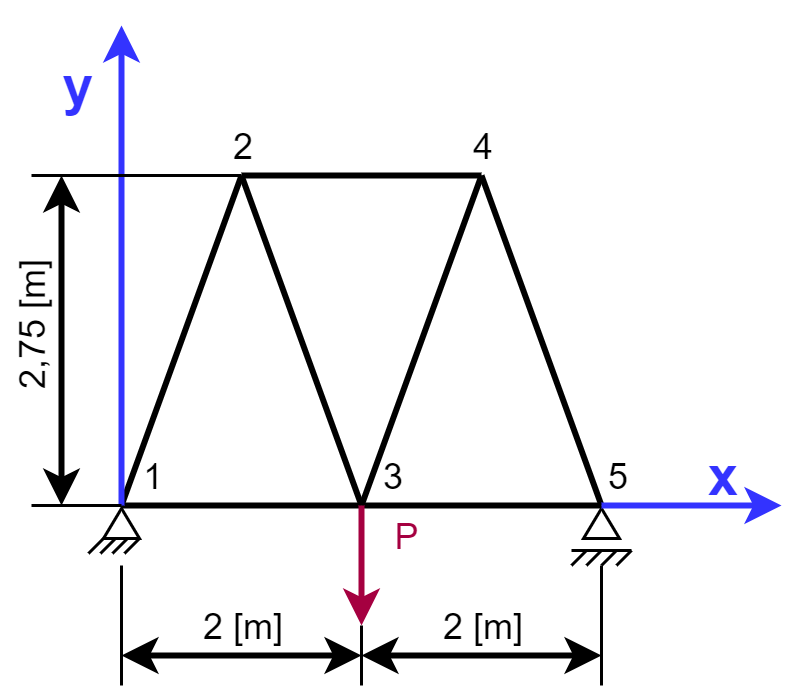
\includegraphics[width=0.7\textwidth, height=0.7\textwidth]{Kratownica.png}
    \caption{Schemat kratownicy.}
    \label{kratownica}
\end{figure}



\begin{table}[H]
\caption{Tabela elementów kratownicy}
\label{tabela:elementy}

\begin{tabular}{|c|c|c|c|c|c|c|c|c|c|c|}
\hline
\multirow{2}{*}{\begin{tabular}[c]{@{}c@{}}Indeks\\ elem.\end{tabular}} & \multicolumn{2}{c|}{\begin{tabular}[c]{@{}c@{}}Węzeł 1\\ $[m]$\end{tabular}} & \multicolumn{2}{c|}{\begin{tabular}[c]{@{}c@{}}Węzeł 2\\ $[m]$\end{tabular}} & \multirow{2}{*}{\begin{tabular}[c]{@{}c@{}}$l$\\ $[m]$\end{tabular}} & \multirow{2}{*}{\begin{tabular}[c]{@{}c@{}}$A$\\ $[m^2]$\end{tabular}} & \multirow{2}{*}{\begin{tabular}[c]{@{}c@{}}$E$\\ $[GPa]$\end{tabular}} & \multirow{2}{*}{\begin{tabular}[c]{@{}c@{}}$\rho{}$\\ $[\frac{kg}{m^3}]$\end{tabular}} & \multicolumn{2}{c|}{Wartość} \\ \cline{2-5} \cline{10-11} 
                                                                        & x                                   & y                                      & x                                   & y                                      &                                                                      &                                                                        &                                                                        &                                                                                        & $cos\theta$   & $sin\theta$  \\ \hline
1                                                                       & 0                                   & 0                                      & 1                                   & 2.75                                   & 2.9262                                                               & 0.00025                                                                & 190                                                                    & 7850                                                                                   & 0.3417        & 0.9398       \\ \hline
2                                                                       & 0                                   & 0                                      & 2                                   & 0                                      & 2                                                                    & 0.00025                                                                & 190                                                                    & 7850                                                                                   & 1             & 0            \\ \hline
3                                                                       & 1                                   & 2.75                                   & 2                                   & 0                                      & 2.9262                                                               & 0.00025                                                                & 190                                                                    & 7850                                                                                   & 0.3417        & -0.9398      \\ \hline
4                                                                       & 1                                   & 2.75                                   & 3                                   & 2.75                                   & 2                                                                    & 0.00025                                                                & 190                                                                    & 7850                                                                                   & 1             & 0            \\ \hline
5                                                                       & 2                                   & 0                                      & 3                                   & 2.75                                   & 2.9262                                                               & 0.00025                                                                & 190                                                                    & 7850                                                                                   & 0.3417        & 0.9398       \\ \hline
6                                                                       & 2                                   & 0                                      & 4                                   & 0                                      & 2                                                                    & 0.00025                                                                & 190                                                                    & 7850                                                                                   & 1             & 0            \\ \hline
7                                                                       & 3                                   & 2.75                                   & 4                                   & 0                                      & 2.9262                                                               & 0.00025                                                                & 190                                                                    & 7850                                                                                   & 0.3417        & -0.9398      \\ \hline
\end{tabular}
\end{table}

\newpage

\subsection{Analiza statyczna}
\label{sec:stat:matlab}

Poniżej przedstawione zostaną macierze sztywności w układzie globalnym dla każdego z elementów.

$$ [k_{1-2}]= 10^7 \cdot \left(\begin{matrix}0.1896&0.5213&-0.1896&-0.5213&0&0&0&0&0&0\\0.5213&1.4337&-0.5213&-1.4337&0&0&0&0&0&0\\-0.1896&-0.5213&0.1896&0.5213&0&0&0&0&0&0\\-0.5213&-1.4337&0.5213&1.4337&0&0&0&0&0&0\\0&0&0&0&0&0&0&0&0&0\\0&0&0&0&0&0&0&0&0&0\\0&0&0&0&0&0&0&0&0&0\\0&0&0&0&0&0&0&0&0&0\\0&0&0&0&0&0&0&0&0&0\\0&0&0&0&0&0&0&0&0&0\end{matrix}\right) $$


$$ [k_{1-3}]= 10^7 \cdot \left(\begin{matrix}2.375&0&0&0&-2.375&0&0&0&0&0\\0&0&0&0&0&0&0&0&0&0\\0&0&0&0&0&0&0&0&0&0\\0&0&0&0&0&0&0&0&0&0\\-2.375&0&0&0&2.375&0&0&0&0&0\\0&0&0&0&0&0&0&0&0&0\\0&0&0&0&0&0&0&0&0&0\\0&0&0&0&0&0&0&0&0&0\\0&0&0&0&0&0&0&0&0&0\\0&0&0&0&0&0&0&0&0&0\end{matrix}\right) $$


$$ [k_{2-3}]= 10^7 \cdot \left(\begin{matrix}0&0&0&0&0&0&0&0&0&0\\0&0&0&0&0&0&0&0&0&0\\0&0&0.1896&-0.5213&-0.1896&0.5213&0&0&0&0\\0&0&-0.5213&1.4337&0.5213&-1.4337&0&0&0&0\\0&0&-0.1896&0.5213&0.1896&-0.5213&0&0&0&0\\0&0&0.5213&-1.4337&-0.5213&1.4337&0&0&0&0\\0&0&0&0&0&0&0&0&0&0\\0&0&0&0&0&0&0&0&0&0\\0&0&0&0&0&0&0&0&0&0\\0&0&0&0&0&0&0&0&0&0\end{matrix}\right) $$


$$ [k_{2-4}]= 10^7 \cdot \left(\begin{matrix}0&0&0&0&0&0&0&0&0&0\\0&0&0&0&0&0&0&0&0&0\\0&0&2.375&0&0&0&-2.375&0&0&0\\0&0&0&0&0&0&0&0&0&0\\0&0&0&0&0&0&0&0&0&0\\0&0&0&0&0&0&0&0&0&0\\0&0&-2.375&0&0&0&2.375&0&0&0\\0&0&0&0&0&0&0&0&0&0\\0&0&0&0&0&0&0&0&0&0\\0&0&0&0&0&0&0&0&0&0\end{matrix}\right) $$

$$ [k_{3-4}]= 10^7 \cdot \left(\begin{matrix}0&0&0&0&0&0&0&0&0&0\\0&0&0&0&0&0&0&0&0&0\\0&0&0&0&0&0&0&0&0&0\\0&0&0&0&0&0&0&0&0&0\\0&0&0&0&0.1896&0.5213&-0.1896&-0.5213&0&0\\0&0&0&0&0.5213&1.4337&-0.5213&-1.4337&0&0\\0&0&0&0&-0.1896&-0.5213&0.1896&0.5213&0&0\\0&0&0&0&-0.5213&-1.4337&0.5213&1.4337&0&0\\0&0&0&0&0&0&0&0&0&0\\0&0&0&0&0&0&0&0&0&0\end{matrix}\right) $$


$$ [k_{4-5}]= 10^7 \cdot \left(\begin{matrix}0&0&0&0&0&0&0&0&0&0\\0&0&0&0&0&0&0&0&0&0\\0&0&0&0&0&0&0&0&0&0\\0&0&0&0&0&0&0&0&0&0\\0&0&0&0&2.375&0&0&0&-2.375&0\\0&0&0&0&0&0&0&0&0&0\\0&0&0&0&0&0&0&0&0&0\\0&0&0&0&0&0&0&0&0&0\\0&0&0&0&-2.375&0&0&0&2.375&0\\0&0&0&0&0&0&0&0&0&0\end{matrix}\right) $$


$$ [k_{3-5}]= 10^7 \cdot \left(\begin{matrix}0&0&0&0&0&0&0&0&0&0\\0&0&0&0&0&0&0&0&0&0\\0&0&0&0&0&0&0&0&0&0\\0&0&0&0&0&0&0&0&0&0\\0&0&0&0&0&0&0&0&0&0\\0&0&0&0&0&0&0&0&0&0\\0&0&0&0&0&0&0.1896&-0.5213&-0.1896&0.5213\\0&0&0&0&0&0&-0.5213&1.4337&0.5213&-1.4337\\0&0&0&0&0&0&-0.1896&0.5213&0.1896&-0.5213\\0&0&0&0&0&0&0.5213&-1.4337&-0.5213&1.4337\end{matrix}\right) $$

\newpage

Macierz sztywności układu po agregacji wygląda następująco.


$$ [k_{g}]= 10^6 \cdot \left(\begin{matrix}25.64&5.21&-1.89&-5.21&-23.75&0&0&0&0&0\\5.21&14.34&-5.21&-14.34&0&0&0&0&0&0\\-1.89&-5.21&27.54&0&-1.89&5.21&-23.75&0&0&0\\-5.21&-14.34&0&28.67&5.21&-14.33&0&0&0&0\\-23.75&0&-1.89&5.21&51.29&0&-1.89&-5.21&-23.75&0\\0&0&5.21&-14.34&0&28.67&-5.21&-14.34&0&0\\0&0&-23.75&0&-1.89&-5.21&27.54&0&-1.89&5.21\\0&0&0&0&-5.21&-14.34&0&28.67&5.21&-14.33\\0&0&0&0&-23.75&0&-1.89&5.21&25.64&-5.21\end{matrix}\right) $$

Po uwzględnieniu warunków brzegowych dla węzła pierwszego na obu kierunkach (wyzerowanie dwóch pierwszych kolumn i wierszów oraz wstawienie $1$ na przecięciu kolumny z wierszem) oraz dla węzła $5$ na kierunku pionowym (ostatni wiersz i kolumna), macierz sztywności układu przyjmuje postać:

$$ [k_{g}]= 10^6 \cdot \left(\begin{matrix} 10^{-6} &0&0&0&0&0&0&0&0&0\\0& 10^{-6} &0&0&0&0&0&0&0&0\\0&0&27.54&0&-1.89&5.21&-23.75&0&0&0\\0&0&0&28.67&5.21&-14.33&0&0&0&0\\0&0&-1.89&5.21&51.29&0&-1.89&-5.21&-23.75&0\\0&0&5.21&-14.34&0&28.67&-5.21&-14.34&0&0\\0&0&-23.75&0&-1.89&-5.21&27.54&0&-1.89&0\\0&0&0&0&-5.21&-14.34&0&28.67&5.21&0\\0&0&0&0&0&0&0&0&0& 10^{-6} \end{matrix}\right) $$

Po rozwiązaniu równania \ref{wzor:mes} otrzymano przemieszczenia węzłów, które  przedstawione są w tabeli \ref{tabela:wynikimatlab}. Przemieszczenia zostały także zobrazowane na rysunku \ref{kratownicawynik}.


\begin{table}[H]
\caption{Przemieszczenia węzłów konstrukcji pod wpływem działania siły}
\label{tabela:wynikimatlab}
\centering
\begin{tabular}{|l|l|l|}
\hline
\multirow{2}{*}{\begin{tabular}[c]{@{}l@{}}Indeks\\ węzła\end{tabular}} & \multicolumn{2}{l|}{Przemieszczenie węzła {[}m{]}} \\ \cline{2-3} 
                                                                        & x                         & y                      \\ \hline
1                                                                       & 0                         & 0                      \\ \hline
2                                                                       & 0.015311                  & -0.040442              \\ \hline
3                                                                       & 0.007655                  & -0.078101              \\ \hline
4                                                                       & -1.31530e-17              & -0.040442              \\ \hline
5                                                                       & 0.015311                  & 0                      \\ \hline
\end{tabular}
\end{table}

\newpage

\begin{figure}[H]
    \centering
    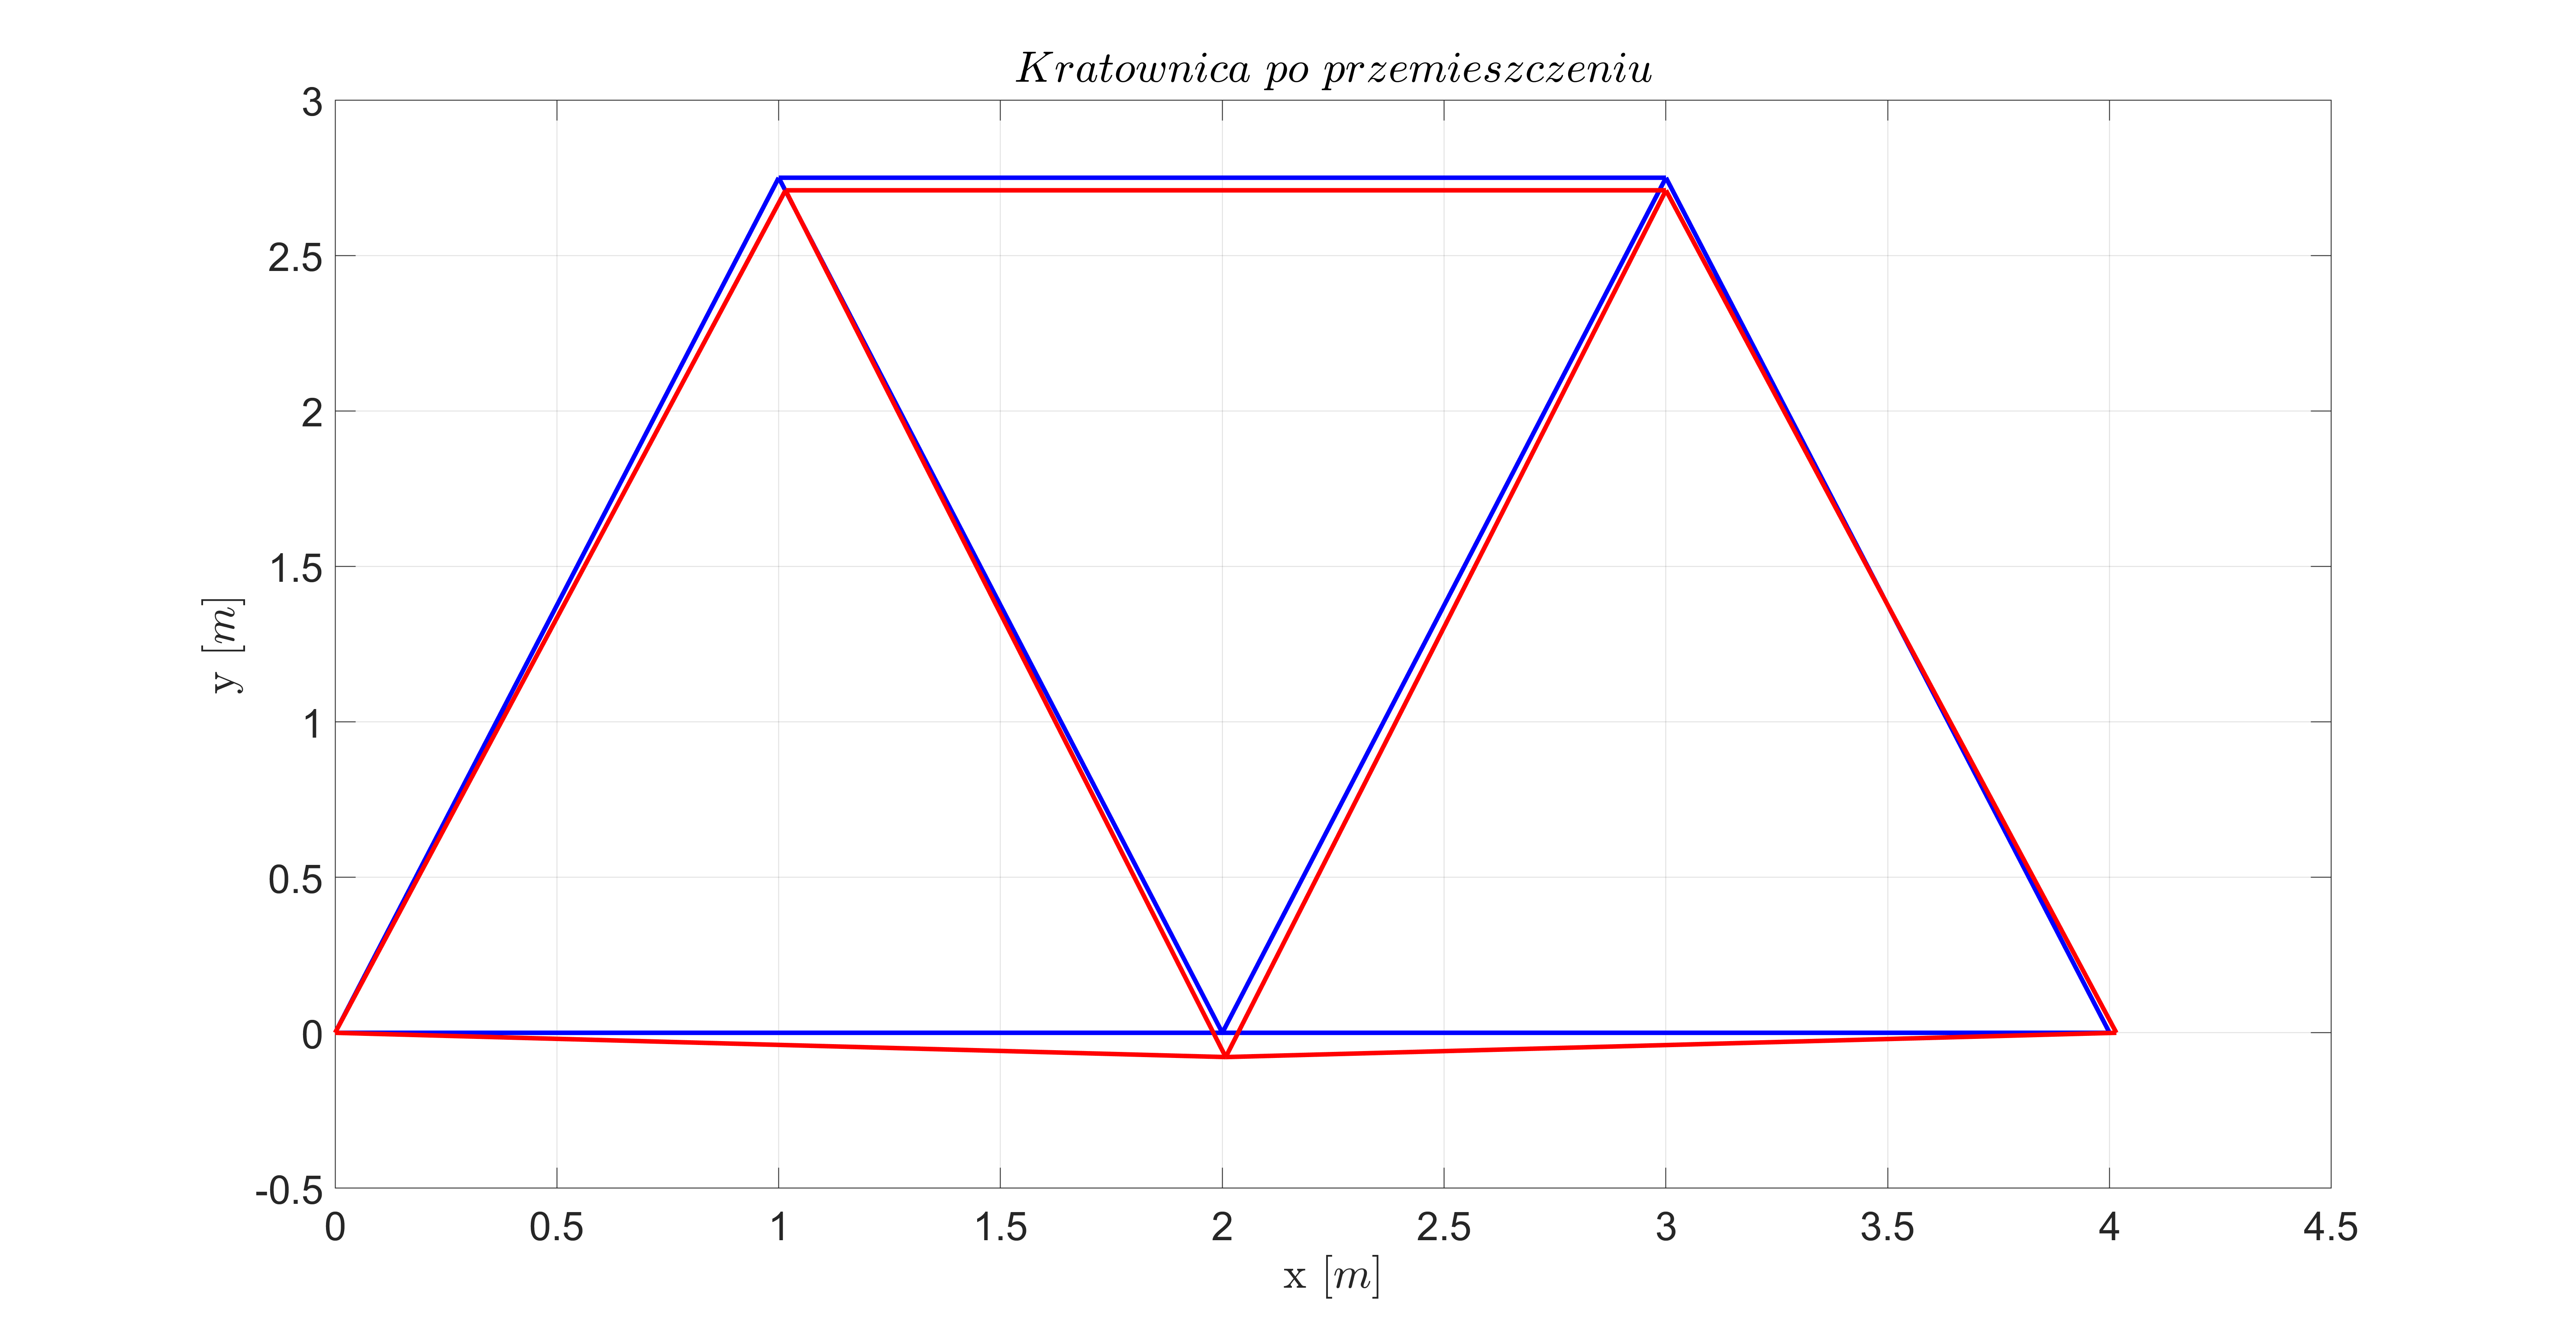
\includegraphics[width=\textwidth, height=0.7\textwidth]{wynik.png}
    \caption{Wykres kratownicy po przemieszczeniu}
    \label{kratownicawynik}
\end{figure}

\subsection{Analiza dynamiczna}
\label{sec:dynam:matlab}

W tym rozdziale dokonana zostanie analiza dynamiczna konstrukcji według metody opisanej w \ref{sec:wstep}. Ponizej przedstawione zostaną macierze bezwładności wszyskich elementów zapisane w układzie globalnym.


$$ [m_{1-2}] = \left(\begin{array}{cccccccccc} 1.91 & 0 & 0.96 & 0 & 0 & 0 & 0 & 0 & 0 & 0\\ 0 & 1.91 & 0 & 0.96 & 0 & 0 & 0 & 0 & 0 & 0\\ 0.96 & 0 & 1.91 & 0 & 0 & 0 & 0 & 0 & 0 & 0\\ 0 & 0.96 & 0 & 1.91 & 0 & 0 & 0 & 0 & 0 & 0\\ 0 & 0 & 0 & 0 & 0 & 0 & 0 & 0 & 0 & 0\\ 0 & 0 & 0 & 0 & 0 & 0 & 0 & 0 & 0 & 0\\ 0 & 0 & 0 & 0 & 0 & 0 & 0 & 0 & 0 & 0\\ 0 & 0 & 0 & 0 & 0 & 0 & 0 & 0 & 0 & 0\\ 0 & 0 & 0 & 0 & 0 & 0 & 0 & 0 & 0 & 0\\ 0 & 0 & 0 & 0 & 0 & 0 & 0 & 0 & 0 & 0 \end{array}\right) $$ 

\newpage

$$ [m_{1-3}] = \left(\begin{array}{cccccccccc} 1.31 & 0 & 0 & 0 & 0.65 & 0 & 0 & 0 & 0 & 0\\ 0 & 1.31 & 0 & 0 & 0 & 0.65 & 0 & 0 & 0 & 0\\ 0 & 0 & 0 & 0 & 0 & 0 & 0 & 0 & 0 & 0\\ 0 & 0 & 0 & 0 & 0 & 0 & 0 & 0 & 0 & 0\\ 0.65 & 0 & 0 & 0 & 1.31 & 0 & 0 & 0 & 0 & 0\\ 0 & 0.65 & 0 & 0 & 0 & 1.31 & 0 & 0 & 0 & 0\\ 0 & 0 & 0 & 0 & 0 & 0 & 0 & 0 & 0 & 0\\ 0 & 0 & 0 & 0 & 0 & 0 & 0 & 0 & 0 & 0\\ 0 & 0 & 0 & 0 & 0 & 0 & 0 & 0 & 0 & 0\\ 0 & 0 & 0 & 0 & 0 & 0 & 0 & 0 & 0 & 0 \end{array}\right) $$

 $$ [m_{2-3}] = \left(\begin{array}{cccccccccc} 0 & 0 & 0 & 0 & 0 & 0 & 0 & 0 & 0 & 0\\ 0 & 0 & 0 & 0 & 0 & 0 & 0 & 0 & 0 & 0\\ 0 & 0 & 1.91 & 0 & 0.96 & 0 & 0 & 0 & 0 & 0\\ 0 & 0 & 0 & 1.91 & 0 & 0.96 & 0 & 0 & 0 & 0\\ 0 & 0 & 0.96 & 0 & 1.91 & 0 & 0 & 0 & 0 & 0\\ 0 & 0 & 0 & 0.96 & 0 & 1.91 & 0 & 0 & 0 & 0\\ 0 & 0 & 0 & 0 & 0 & 0 & 0 & 0 & 0 & 0\\ 0 & 0 & 0 & 0 & 0 & 0 & 0 & 0 & 0 & 0\\ 0 & 0 & 0 & 0 & 0 & 0 & 0 & 0 & 0 & 0\\ 0 & 0 & 0 & 0 & 0 & 0 & 0 & 0 & 0 & 0 \end{array}\right) $$


  $$ [m_{2-4}] = \left(\begin{array}{cccccccccc} 0 & 0 & 0 & 0 & 0 & 0 & 0 & 0 & 0 & 0\\ 0 & 0 & 0 & 0 & 0 & 0 & 0 & 0 & 0 & 0\\ 0 & 0 & 1.31 & 0 & 0 & 0 & 0.65 & 0 & 0 & 0\\ 0 & 0 & 0 & 1.31 & 0 & 0 & 0 & 0.65 & 0 & 0\\ 0 & 0 & 0 & 0 & 0 & 0 & 0 & 0 & 0 & 0\\ 0 & 0 & 0 & 0 & 0 & 0 & 0 & 0 & 0 & 0\\ 0 & 0 & 0.65 & 0 & 0 & 0 & 1.31 & 0 & 0 & 0\\ 0 & 0 & 0 & 0.65 & 0 & 0 & 0 & 1.31 & 0 & 0\\ 0 & 0 & 0 & 0 & 0 & 0 & 0 & 0 & 0 & 0\\ 0 & 0 & 0 & 0 & 0 & 0 & 0 & 0 & 0 & 0 \end{array}\right) $$

 $$ [m_{3-4}] = \left(\begin{array}{cccccccccc} 0 & 0 & 0 & 0 & 0 & 0 & 0 & 0 & 0 & 0\\ 0 & 0 & 0 & 0 & 0 & 0 & 0 & 0 & 0 & 0\\ 0 & 0 & 0 & 0 & 0 & 0 & 0 & 0 & 0 & 0\\ 0 & 0 & 0 & 0 & 0 & 0 & 0 & 0 & 0 & 0\\ 0 & 0 & 0 & 0 & 1.91 & 0 & 0.96 & 0 & 0 & 0\\ 0 & 0 & 0 & 0 & 0 & 1.91 & 0 & 0.96 & 0 & 0\\ 0 & 0 & 0 & 0 & 0.96 & 0 & 1.91 & 0 & 0 & 0\\ 0 & 0 & 0 & 0 & 0 & 0.96 & 0 & 1.91 & 0 & 0\\ 0 & 0 & 0 & 0 & 0 & 0 & 0 & 0 & 0 & 0\\ 0 & 0 & 0 & 0 & 0 & 0 & 0 & 0 & 0 & 0 \end{array}\right) $$

$$ [m_{4-5}] = \left(\begin{array}{cccccccccc} 0 & 0 & 0 & 0 & 0 & 0 & 0 & 0 & 0 & 0\\ 0 & 0 & 0 & 0 & 0 & 0 & 0 & 0 & 0 & 0\\ 0 & 0 & 0 & 0 & 0 & 0 & 0 & 0 & 0 & 0\\ 0 & 0 & 0 & 0 & 0 & 0 & 0 & 0 & 0 & 0\\ 0 & 0 & 0 & 0 & 1.31 & 0 & 0 & 0 & 0.65 & 0\\ 0 & 0 & 0 & 0 & 0 & 1.31 & 0 & 0 & 0 & 0.65\\ 0 & 0 & 0 & 0 & 0 & 0 & 0 & 0 & 0 & 0\\ 0 & 0 & 0 & 0 & 0 & 0 & 0 & 0 & 0 & 0\\ 0 & 0 & 0 & 0 & 0.65 & 0 & 0 & 0 & 1.31 & 0\\ 0 & 0 & 0 & 0 & 0 & 0.65 & 0 & 0 & 0 & 1.31 \end{array}\right) $$

$$ [m_{3-5}] =\left(\begin{array}{cccccccccc} 0 & 0 & 0 & 0 & 0 & 0 & 0 & 0 & 0 & 0\\ 0 & 0 & 0 & 0 & 0 & 0 & 0 & 0 & 0 & 0\\ 0 & 0 & 0 & 0 & 0 & 0 & 0 & 0 & 0 & 0\\ 0 & 0 & 0 & 0 & 0 & 0 & 0 & 0 & 0 & 0\\ 0 & 0 & 0 & 0 & 0 & 0 & 0 & 0 & 0 & 0\\ 0 & 0 & 0 & 0 & 0 & 0 & 0 & 0 & 0 & 0\\ 0 & 0 & 0 & 0 & 0 & 0 & 1.91 & 0 & 0.96 & 0\\ 0 & 0 & 0 & 0 & 0 & 0 & 0 & 1.91 & 0 & 0.96\\ 0 & 0 & 0 & 0 & 0 & 0 & 0.96 & 0 & 1.91 & 0\\ 0 & 0 & 0 & 0 & 0 & 0 & 0 & 0.96 & 0 & 1.91 \end{array}\right) $$

Macierz bezwładności po agregacji przyjumje poniższą postać.

$$ [m_{g}] = \left(\begin{array}{cccccccccc} 3.22 & 0 & 0.96 & 0 & 0.65 & 0 & 0 & 0 & 0 & 0\\ 0 & 3.22 & 0 & 0.96 & 0 & 0.65 & 0 & 0 & 0 & 0\\ 0.96 & 0 & 5.14 & 0 & 0.96 & 0 & 0.65 & 0 & 0 & 0\\ 0 & 0.96 & 0 & 5.14 & 0 & 0.96 & 0 & 0.65 & 0 & 0\\ 0.65 & 0 & 0.96 & 0 & 6.44 & 0 & 0.96 & 0 & 0.65 & 0\\ 0 & 0.65 & 0 & 0.96 & 0 & 6.44 & 0 & 0.96 & 0 & 0.65\\ 0 & 0 & 0.65 & 0 & 0.96 & 0 & 5.14 & 0 & 0.96 & 0\\ 0 & 0 & 0 & 0.65 & 0 & 0.96 & 0 & 5.14 & 0 & 0.96\\ 0 & 0 & 0 & 0 & 0.65 & 0 & 0.96 & 0 & 3.22 & 0\\ 0 & 0 & 0 & 0 & 0 & 0.65 & 0 & 0.96 & 0 & 3.22 \end{array}\right) $$

\newpage

Następnie po uwzględnieniu podobnie jak w przypadku macierzy sztywności warunków brzegowych macierz mas kształtuje się następująco.

$$ [m_{g}] = \left(\begin{array}{cccccccccc} 1.00 & 0 & 0 & 0 & 0 & 0 & 0 & 0 & 0 & 0\\ 0 & 1.00 & 0 & 0 & 0 & 0 & 0 & 0 & 0 & 0\\ 0 & 0 & 5.1 & 0 & 0.96 & 0 & 0.65 & 0 & 0 & 0\\ 0 & 0 & 0 & 5.1 & 0 & 0.96 & 0 & 0.65 & 0 & 0\\ 0 & 0 & 0.96 & 0 & 6.4 & 0 & 0.96 & 0 & 0.65 & 0\\ 0 & 0 & 0 & 0.96 & 0 & 6.4 & 0 & 0.96 & 0 & 0\\ 0 & 0 & 0.65 & 0 & 0.96 & 0 & 5.1 & 0 & 0.96 & 0\\ 0 & 0 & 0 & 0.65 & 0 & 0.96 & 0 & 5.1 & 0 & 0\\ 0 & 0 & 0 & 0 & 0.65 & 0 & 0.96 & 0 & 3.2 & 0\\ 0 & 0 & 0 & 0 & 0 & 0 & 0 & 0 & 0 & 1.00 \end{array}\right) $$

Wyznaczenie wektorów własnych oraz wartości własnych obyło się za pomocą polecania $[V, \lambda] = eig(K, M)$, która zwraca macierz wektorów własnych $V$ oraz wektor wartości własnych $\lambda$. Otrzymane wartości własne należały przeliczyć na częstotliwość wg. wzoru \ref{przeliczenielmabda}. Poniżej przedstawione zostaną odpowiednio wektor częstotliwości własnych oraz macierz wektorów własnych (kolumny) odpowiadających kolejnym częstotliwościom. Pierwsze 3 wartości własne oraz wektory własne zostały pominięte ze względu, iż są one wynikiem zastosowanego sposobu uwzględniania warunków brzegowych (postacie te zakładają przemiesczenie uwierdzonych węzłów).

$$ f = \left(\begin{array}{c}  106.02\\ 159.13\\ 275.69\\ 391.49\\ 494.66\\ 549.19\\ 656.60 \end{array}\right) [Hz] \ \  \Phi = \left(\begin{array}{cccccc} 0 & 0 & 0 & 0 & 0 & 0\\ 0 & 0 & 0 & 0 & 0 & 0\\ -0.26 & 0.037 & 0.18 & -0.022 & 0.14 & -0.23\\ 0.037 & 0.17 & 0.018 & 0.32 & 0.25 & 0.092\\ -0.08 & -0.019 & -0.25 & -0.045 & 0.099 & -0.11\\ 0.037 & 0.25 & -0.058 & 0.016 & -0.24 & -0.19\\ -0.25 & 0.09 & 0.12 & 0.018 & -0.18 & 0.27\\ 0.027 & 0.18 & -0.031 & -0.33 & 0.17 & 0.15\\ -0.11 & -0.051 & -0.36 & 0.1 & -8.4e-3 & 0.068\\ 0 & 0 & 0 & 0 & 0 & 0 \end{array}\right) $$

Poniżej przedstawione zostaną poszczególne postacie drgań (mody) wyznaczone na podstawie wektorów własnych.
\newpage


\begin{figure}[H]
    \centering
    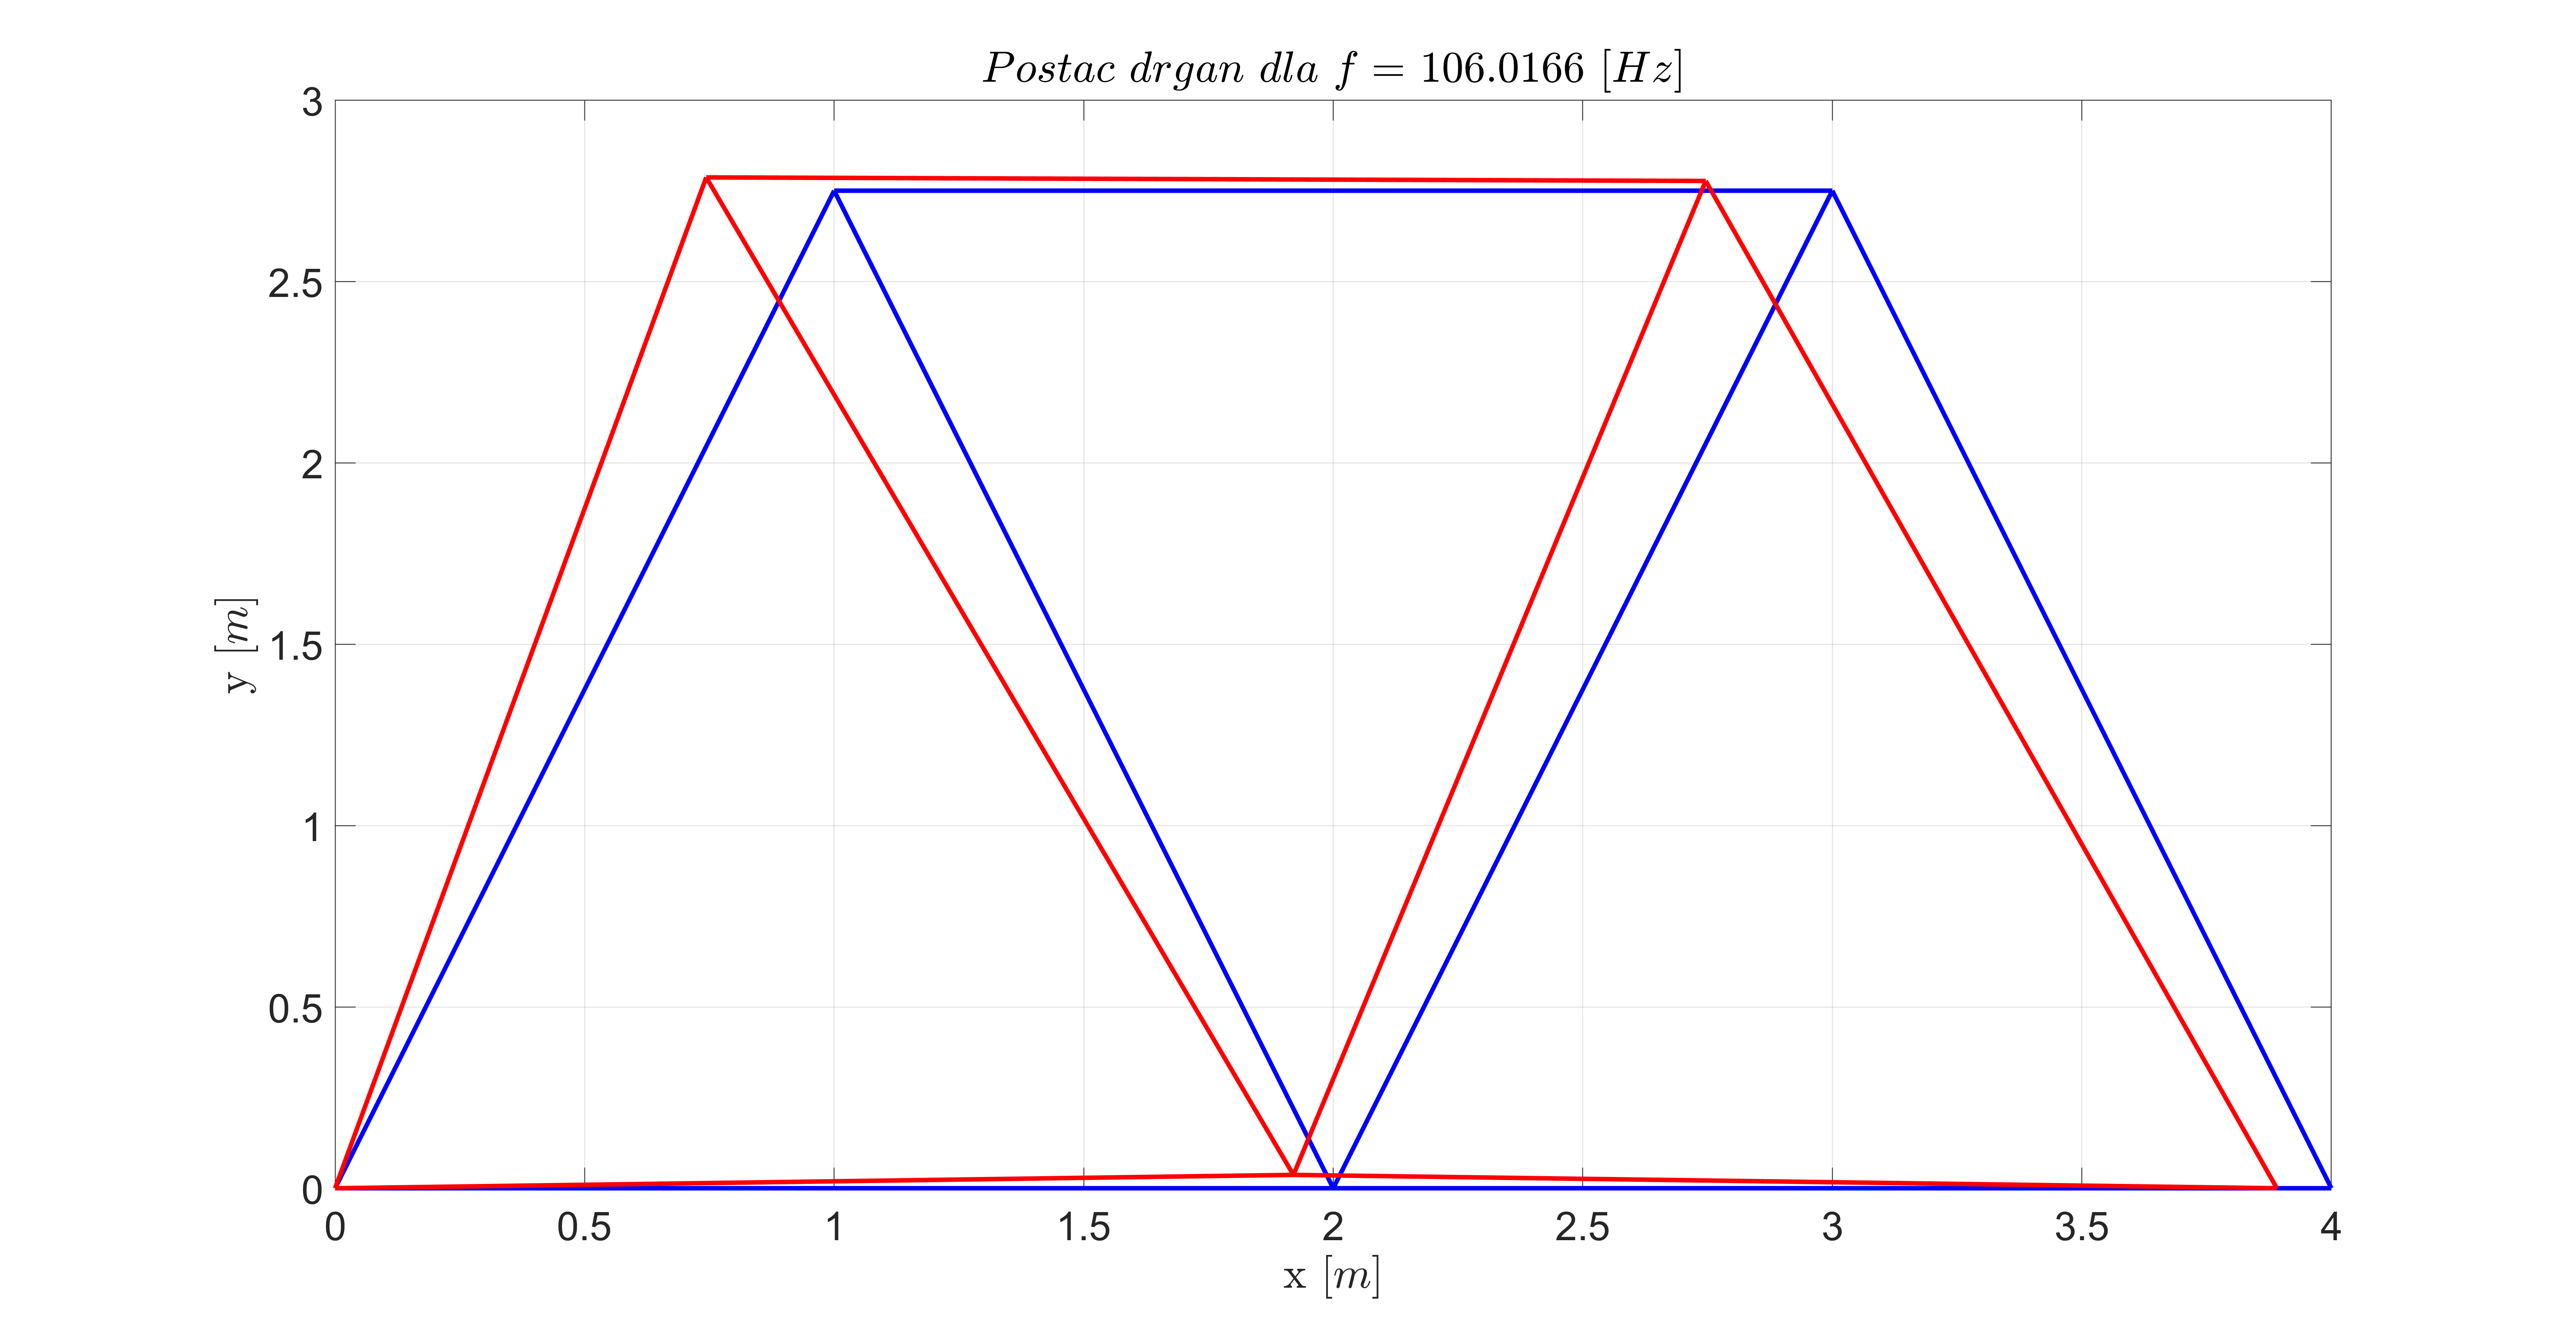
\includegraphics[width=\textwidth, height=0.6\textwidth]{postac_dragn_1.png}
    \caption{Kształt pierwszej postaci dragń}
    \label{postac1}
\end{figure}

\begin{figure}[H]
    \centering
    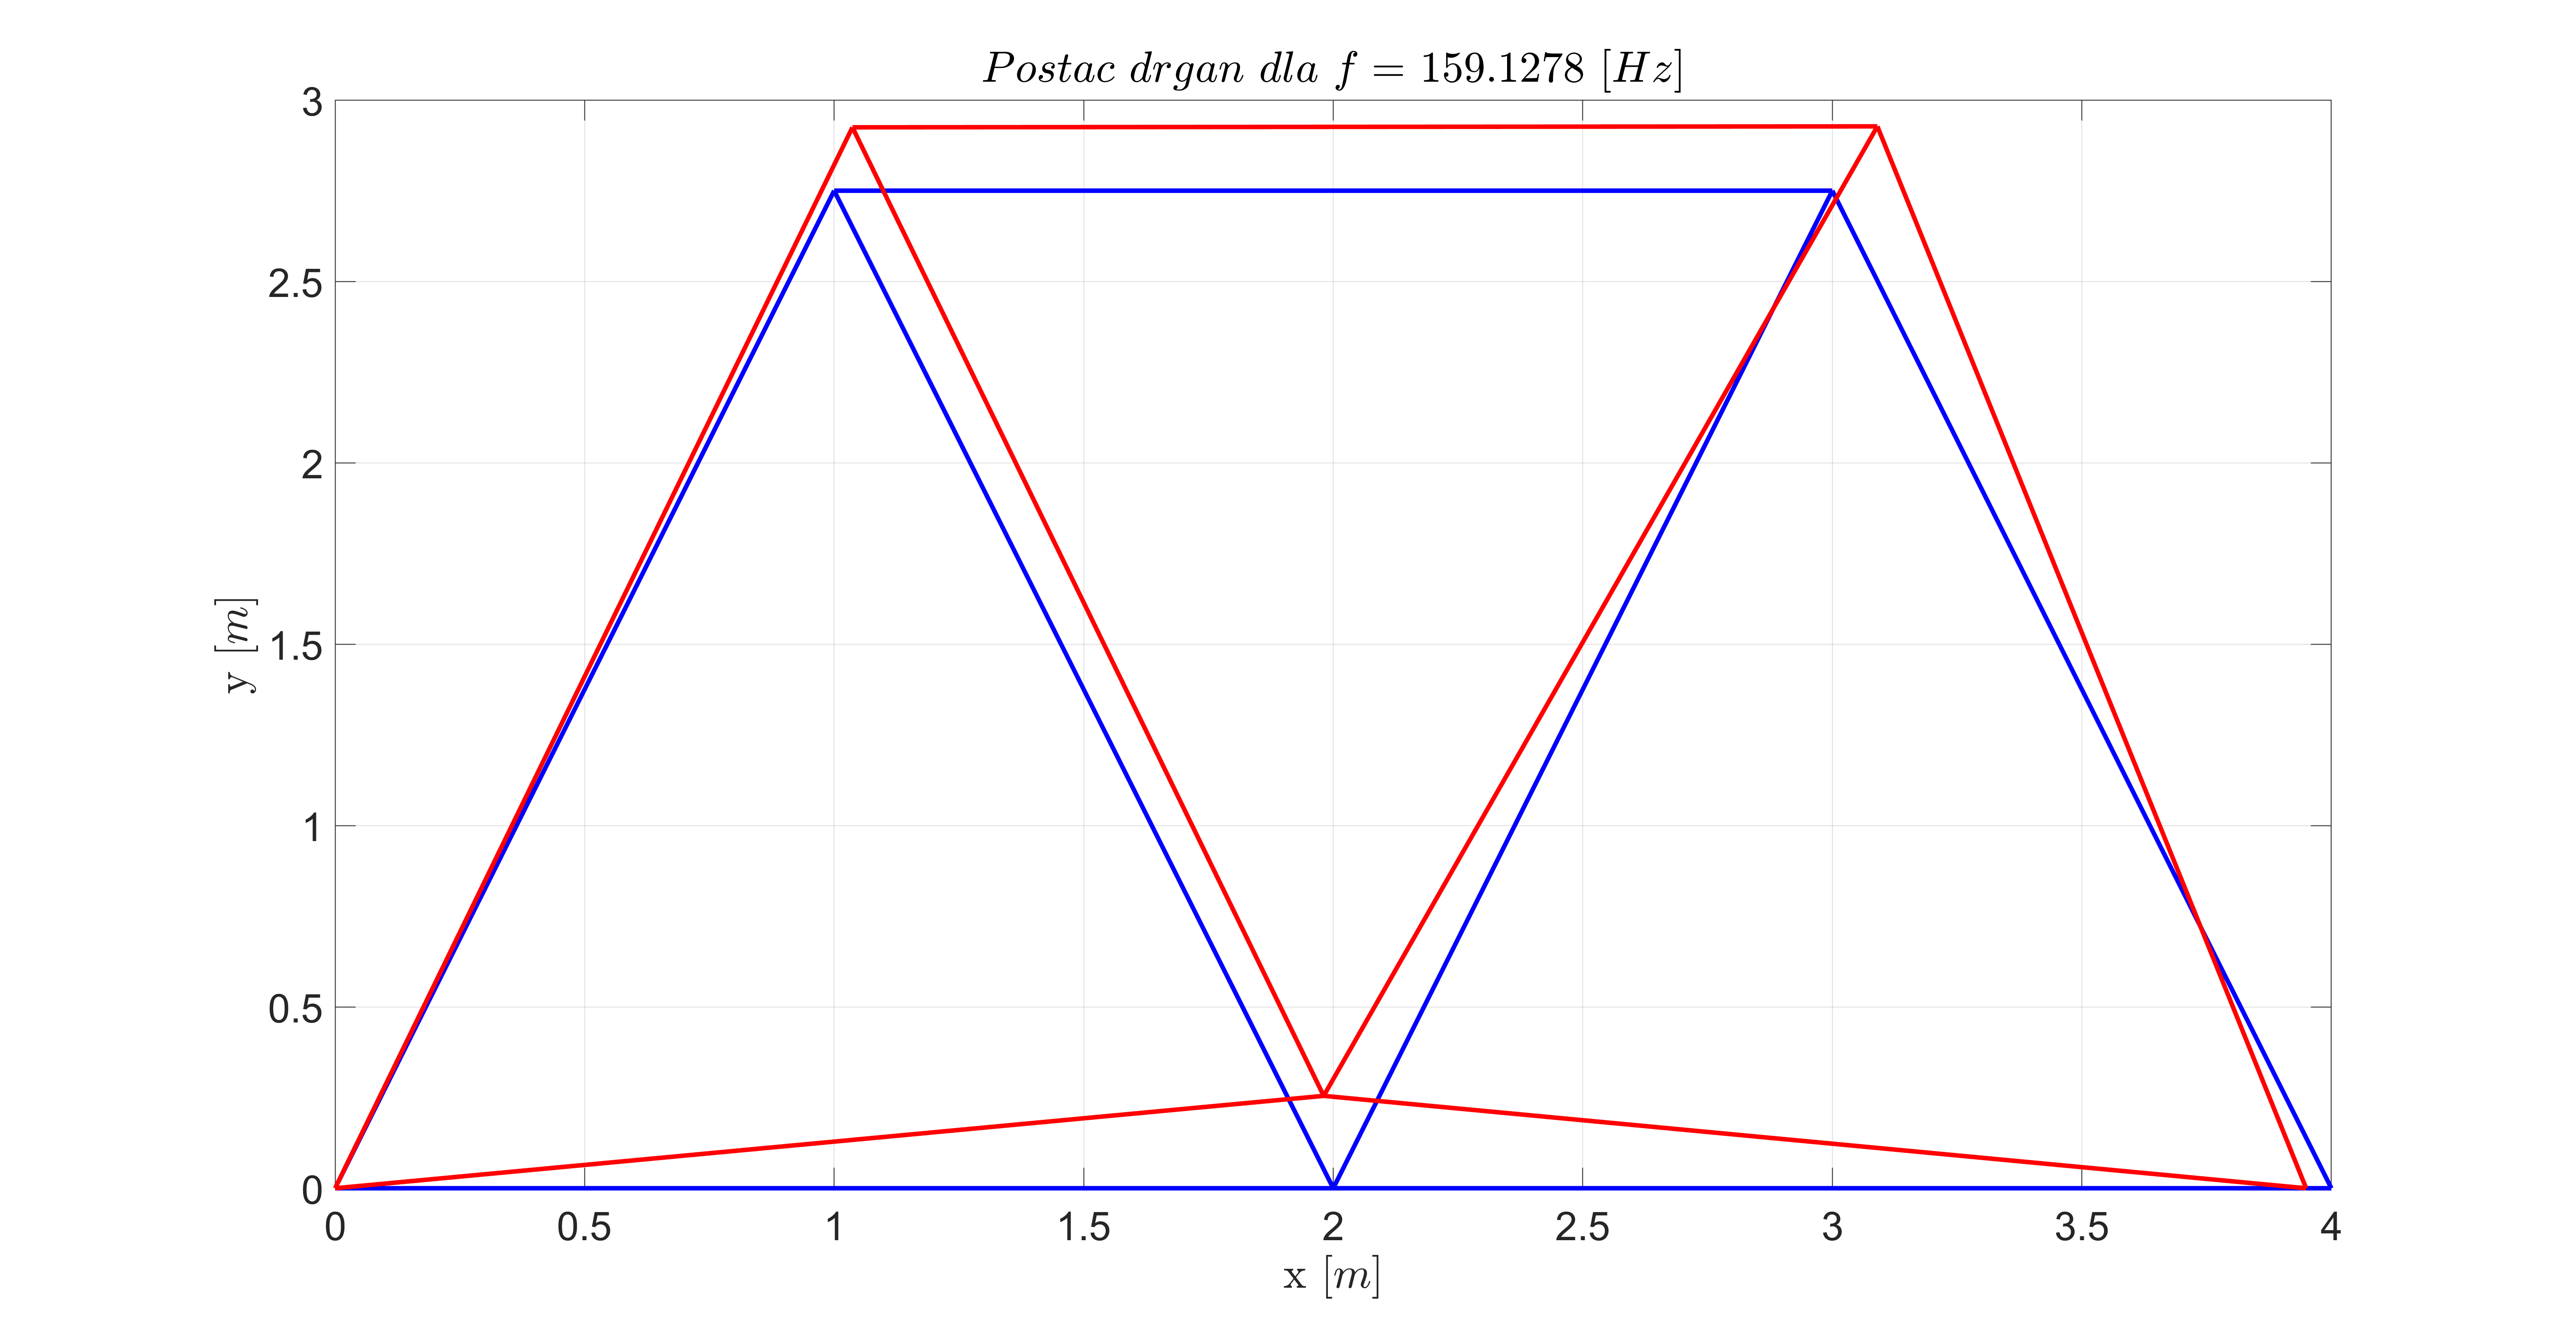
\includegraphics[width=\textwidth, height=0.6\textwidth]{postac_dragn_2.png}
    \caption{Kształt drugiej postaci dragń}
    \label{postac2}
\end{figure}

\begin{figure}[H]
    \centering
    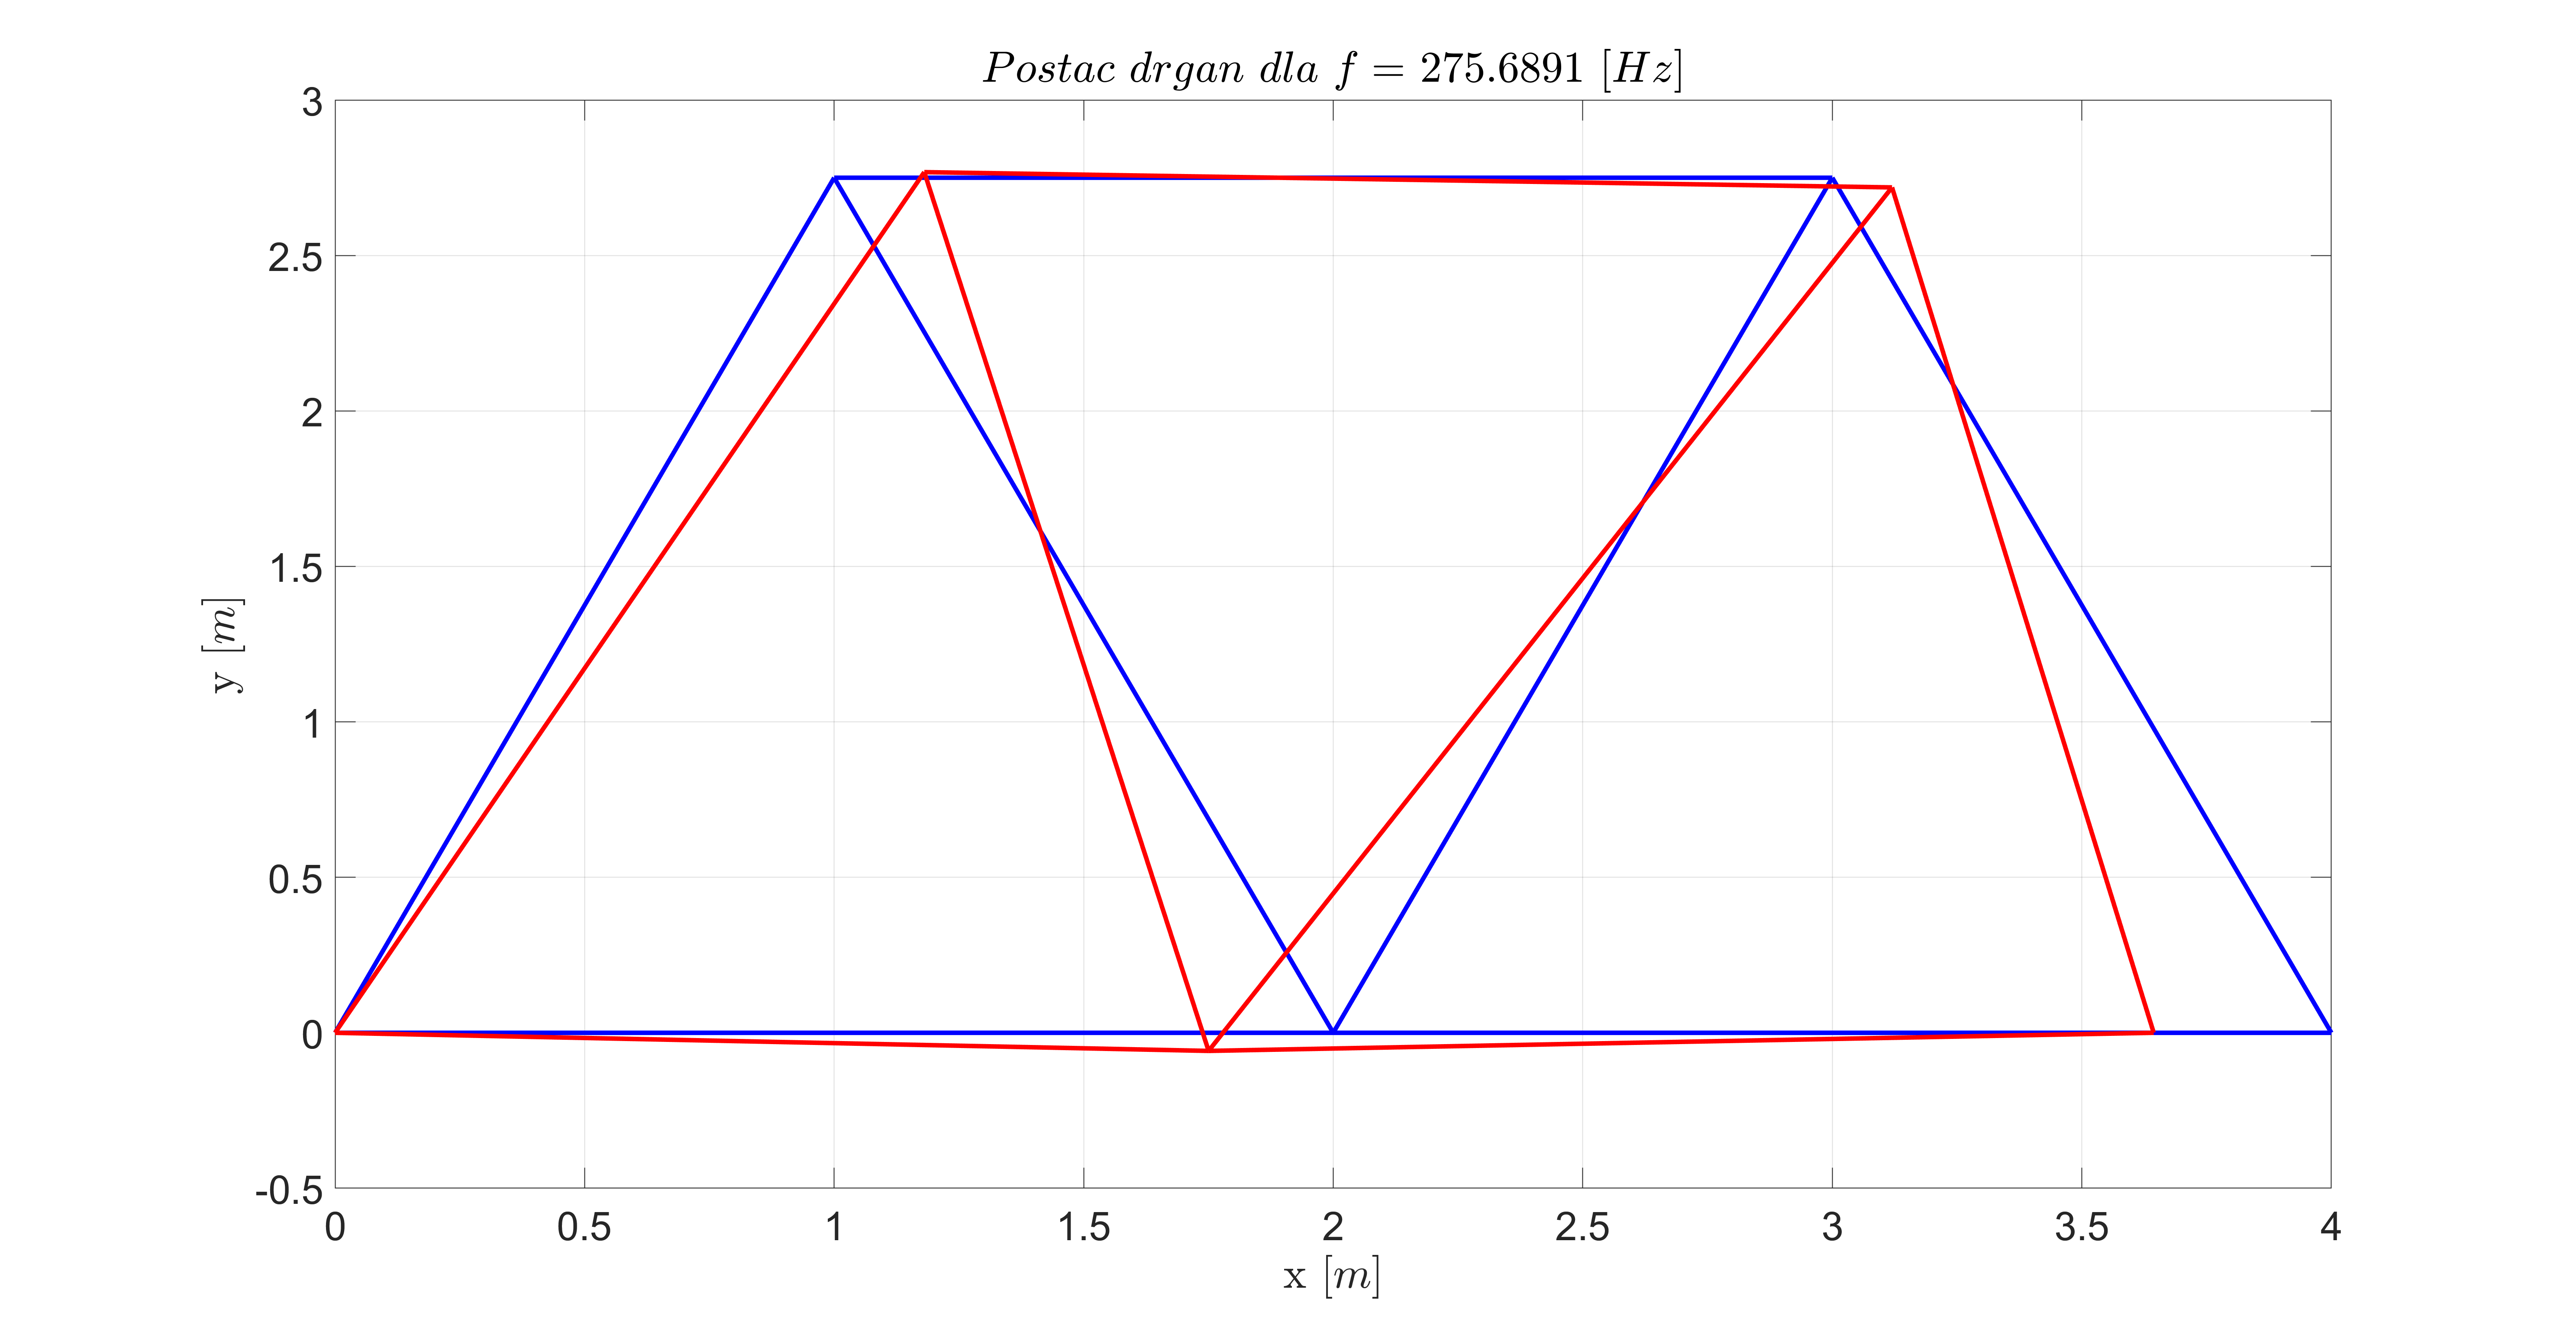
\includegraphics[width=\textwidth, height=0.6\textwidth]{postac_dragn_3.png}
    \caption{Kształt trzeciej postaci dragń}
    \label{postac3}
\end{figure}

\begin{figure}[H]
    \centering
    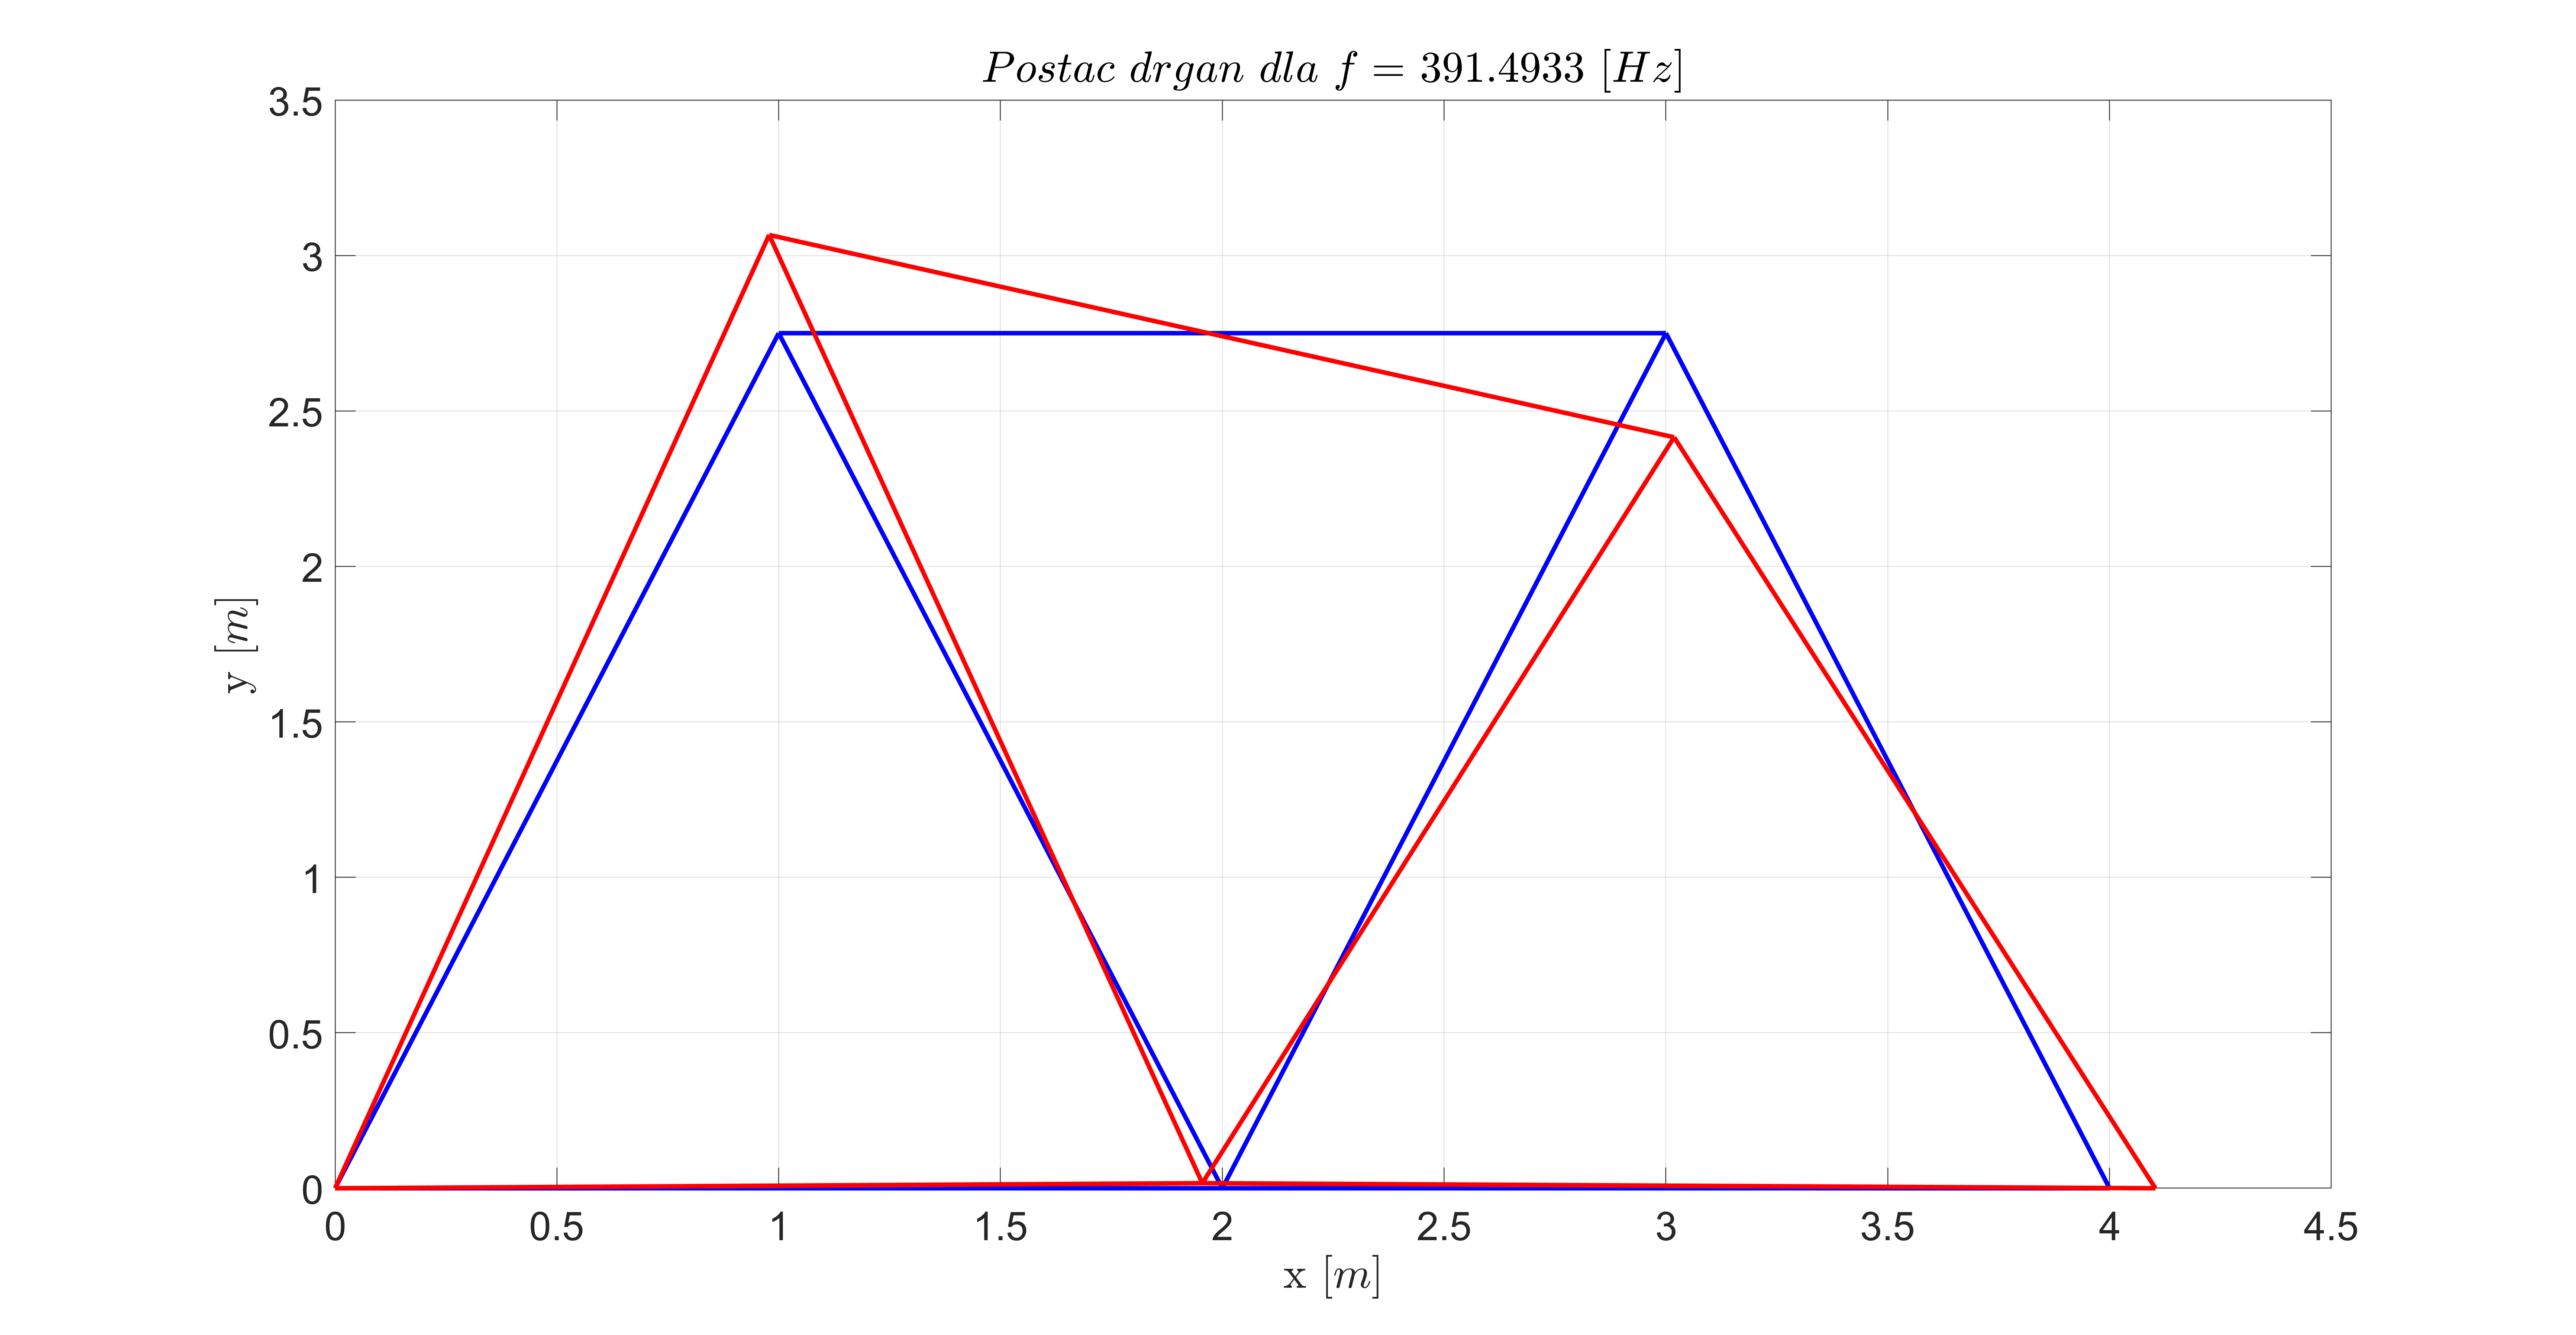
\includegraphics[width=\textwidth, height=0.6\textwidth]{postac_dragn_4.png}
    \caption{Kształt czwartej postaci dragń}
    \label{postac4}
\end{figure}

\begin{figure}[H]
    \centering
    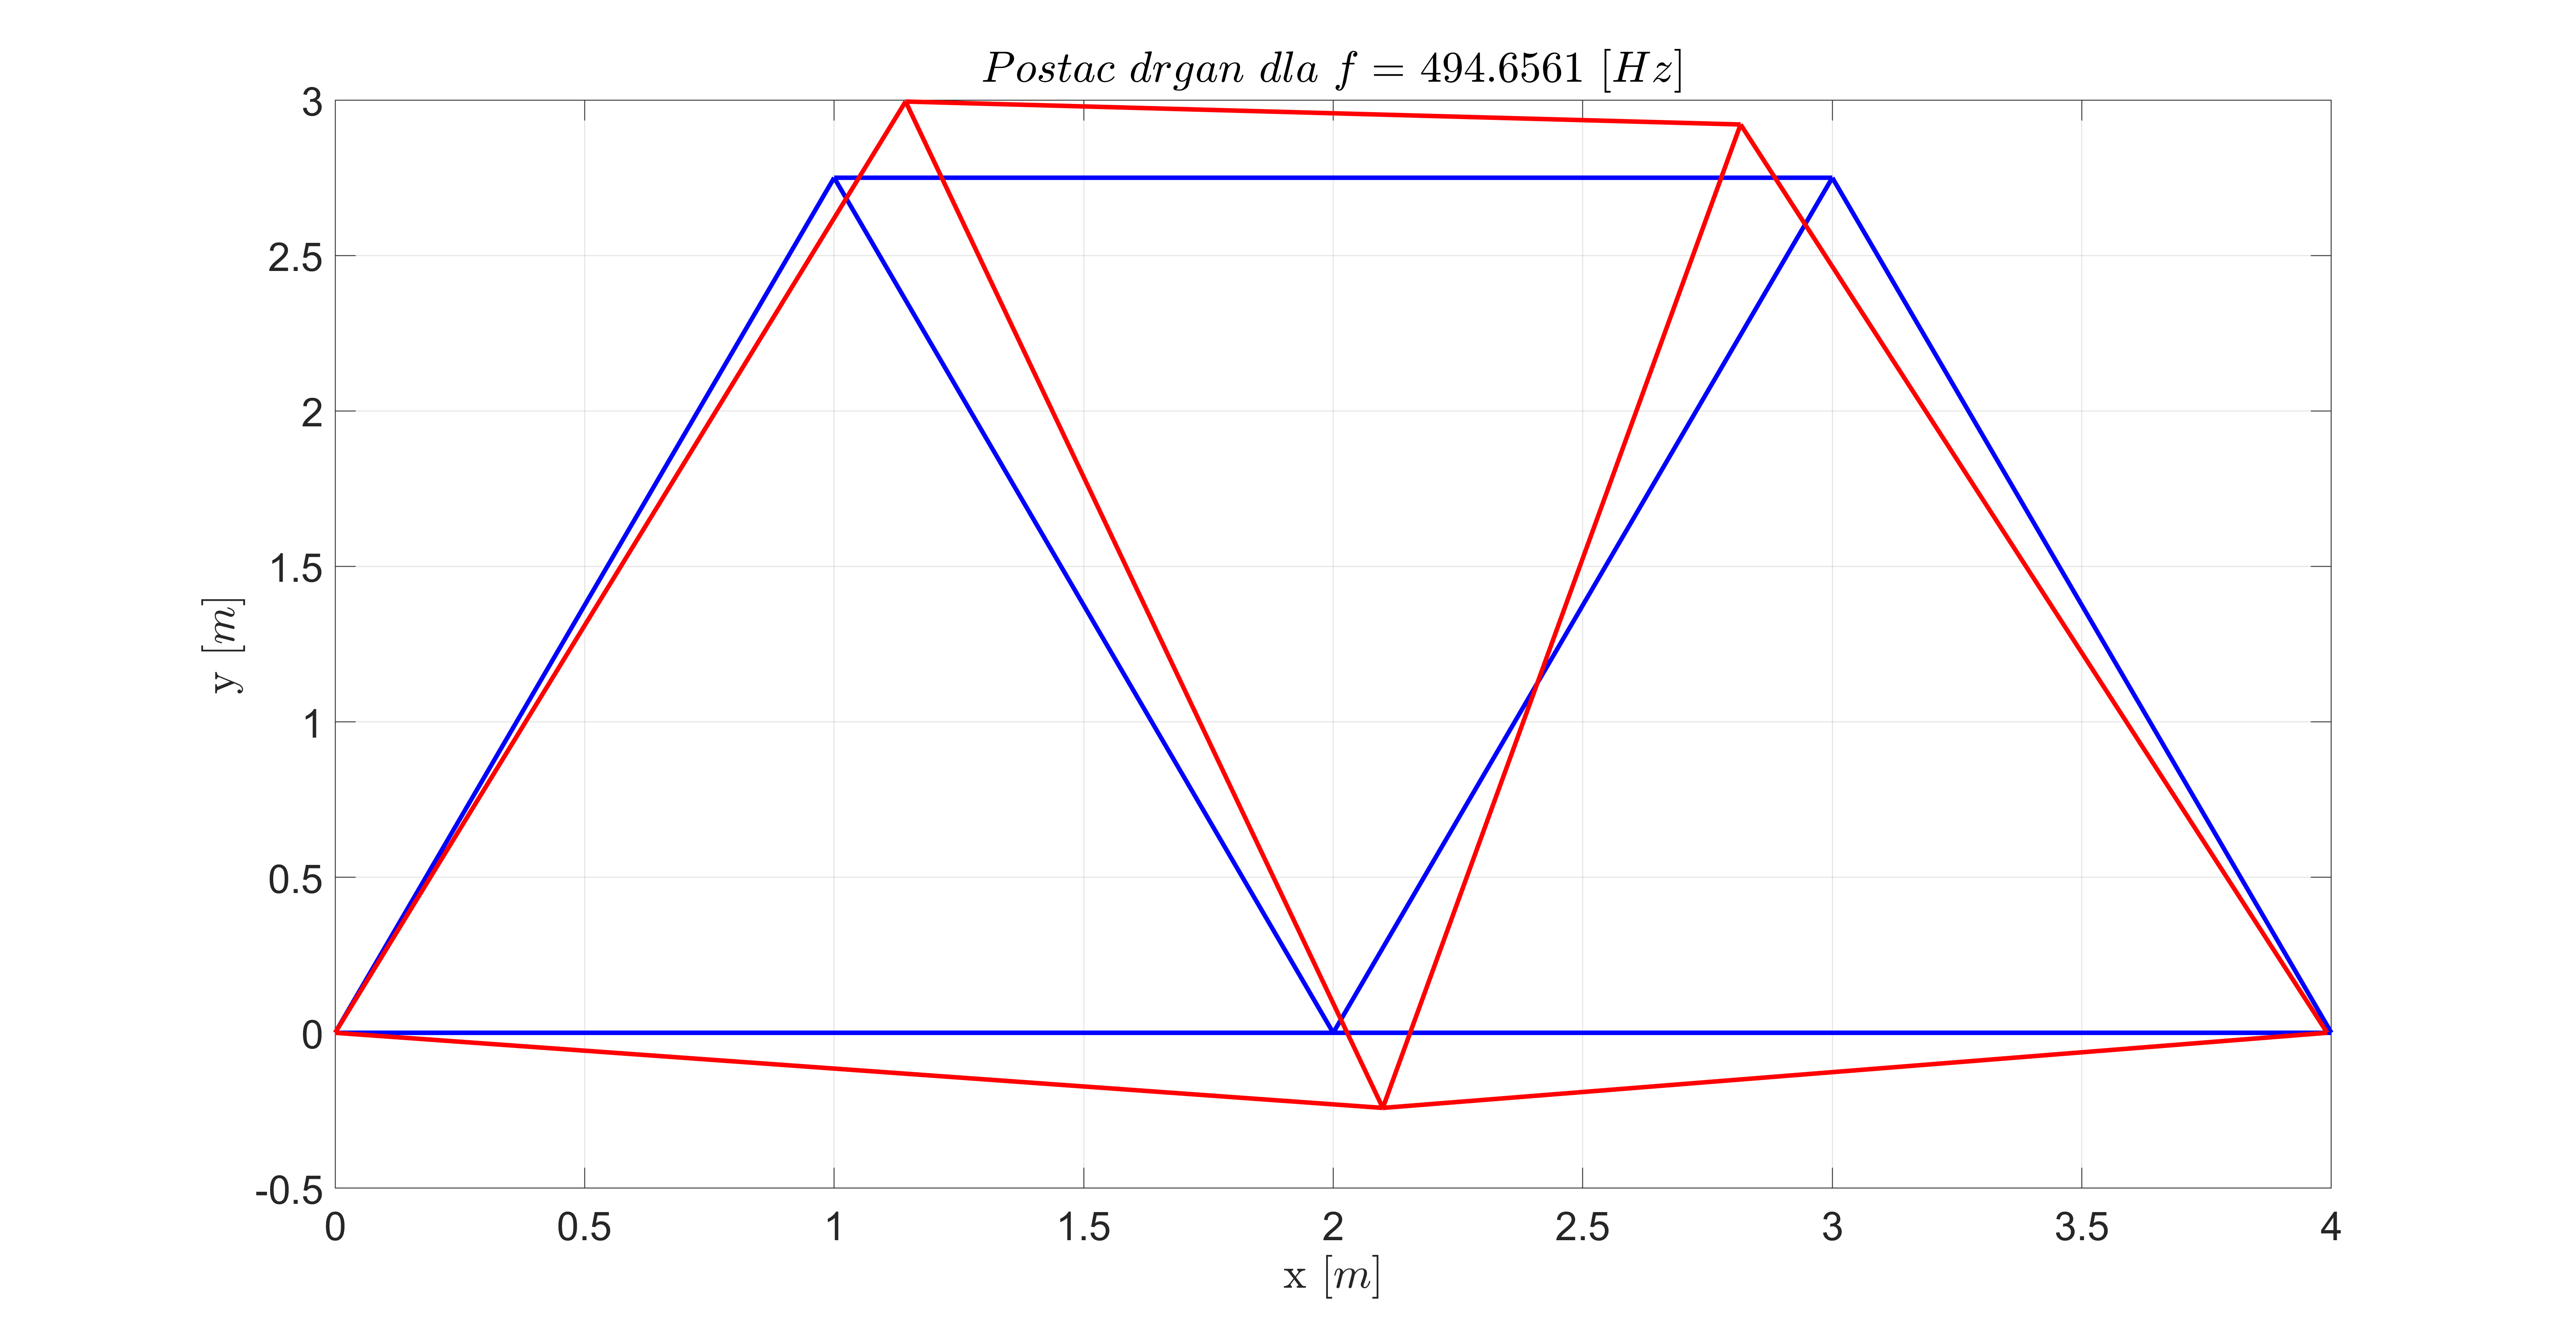
\includegraphics[width=\textwidth, height=0.6\textwidth]{postac_dragn_5.png}
    \caption{Kształt piątej postaci dragń}
    \label{postac5}
\end{figure}

\begin{figure}[H]
    \centering
    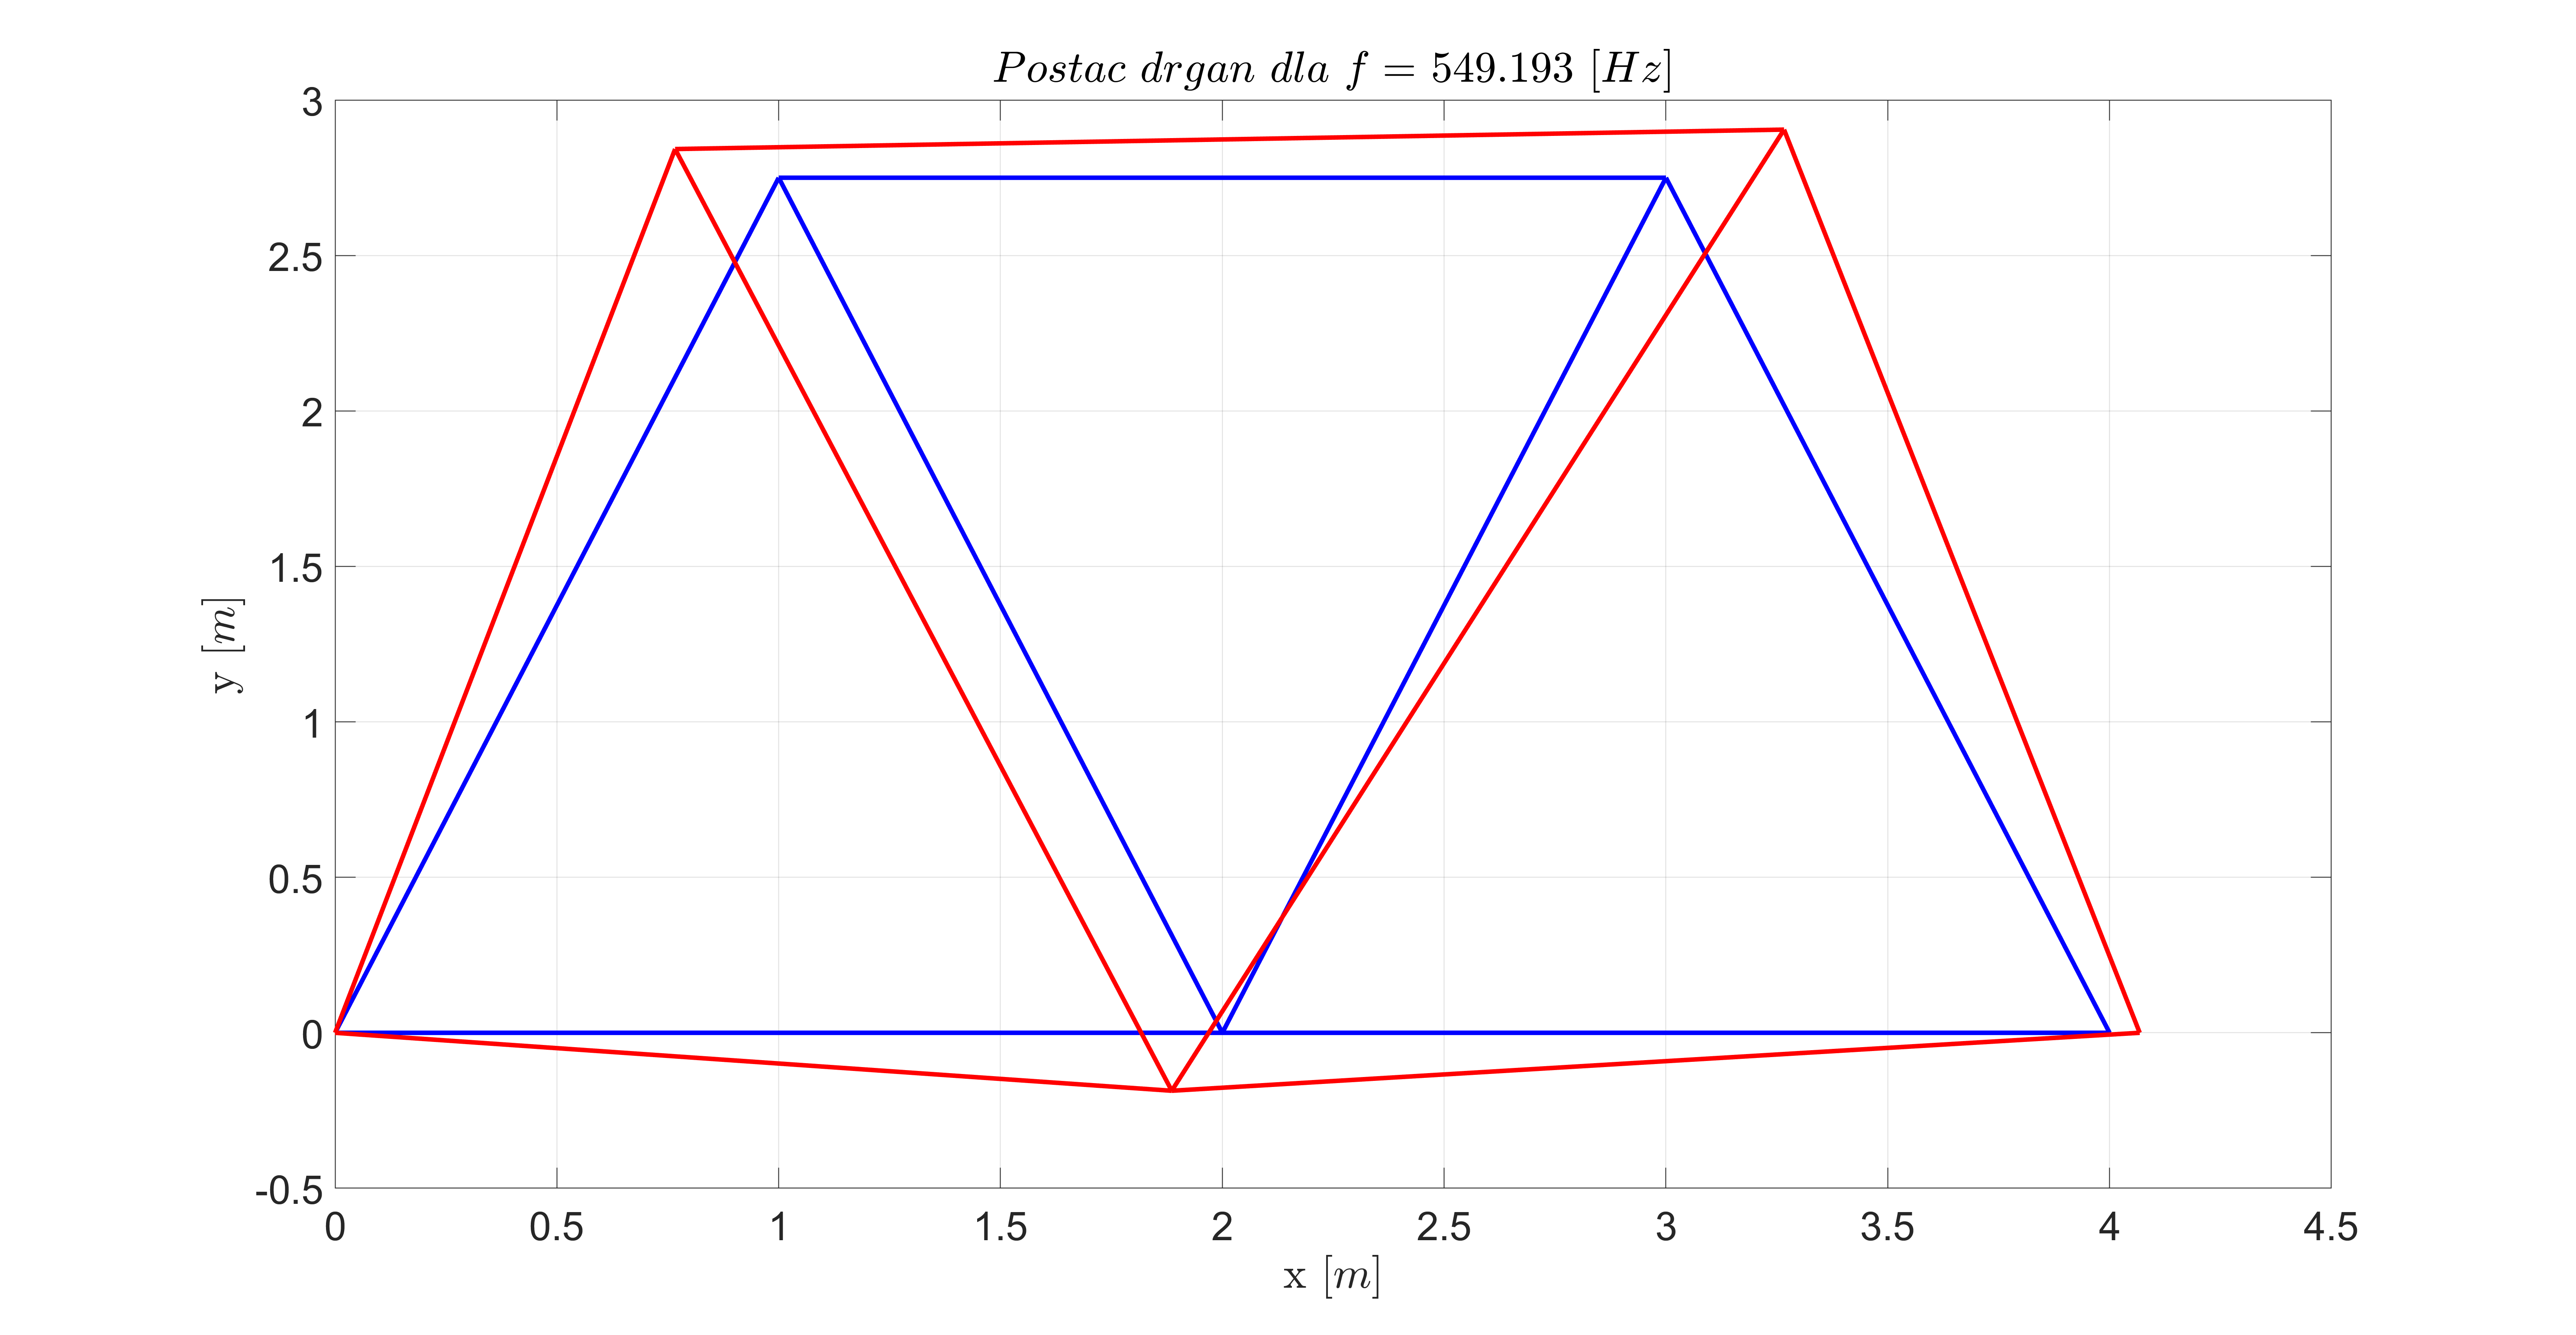
\includegraphics[width=\textwidth, height=0.6\textwidth]{postac_dragn_6.png}
    \caption{Kształt szóstej postaci dragń}
    \label{postac6}
\end{figure}

\begin{figure}[H]
    \centering
    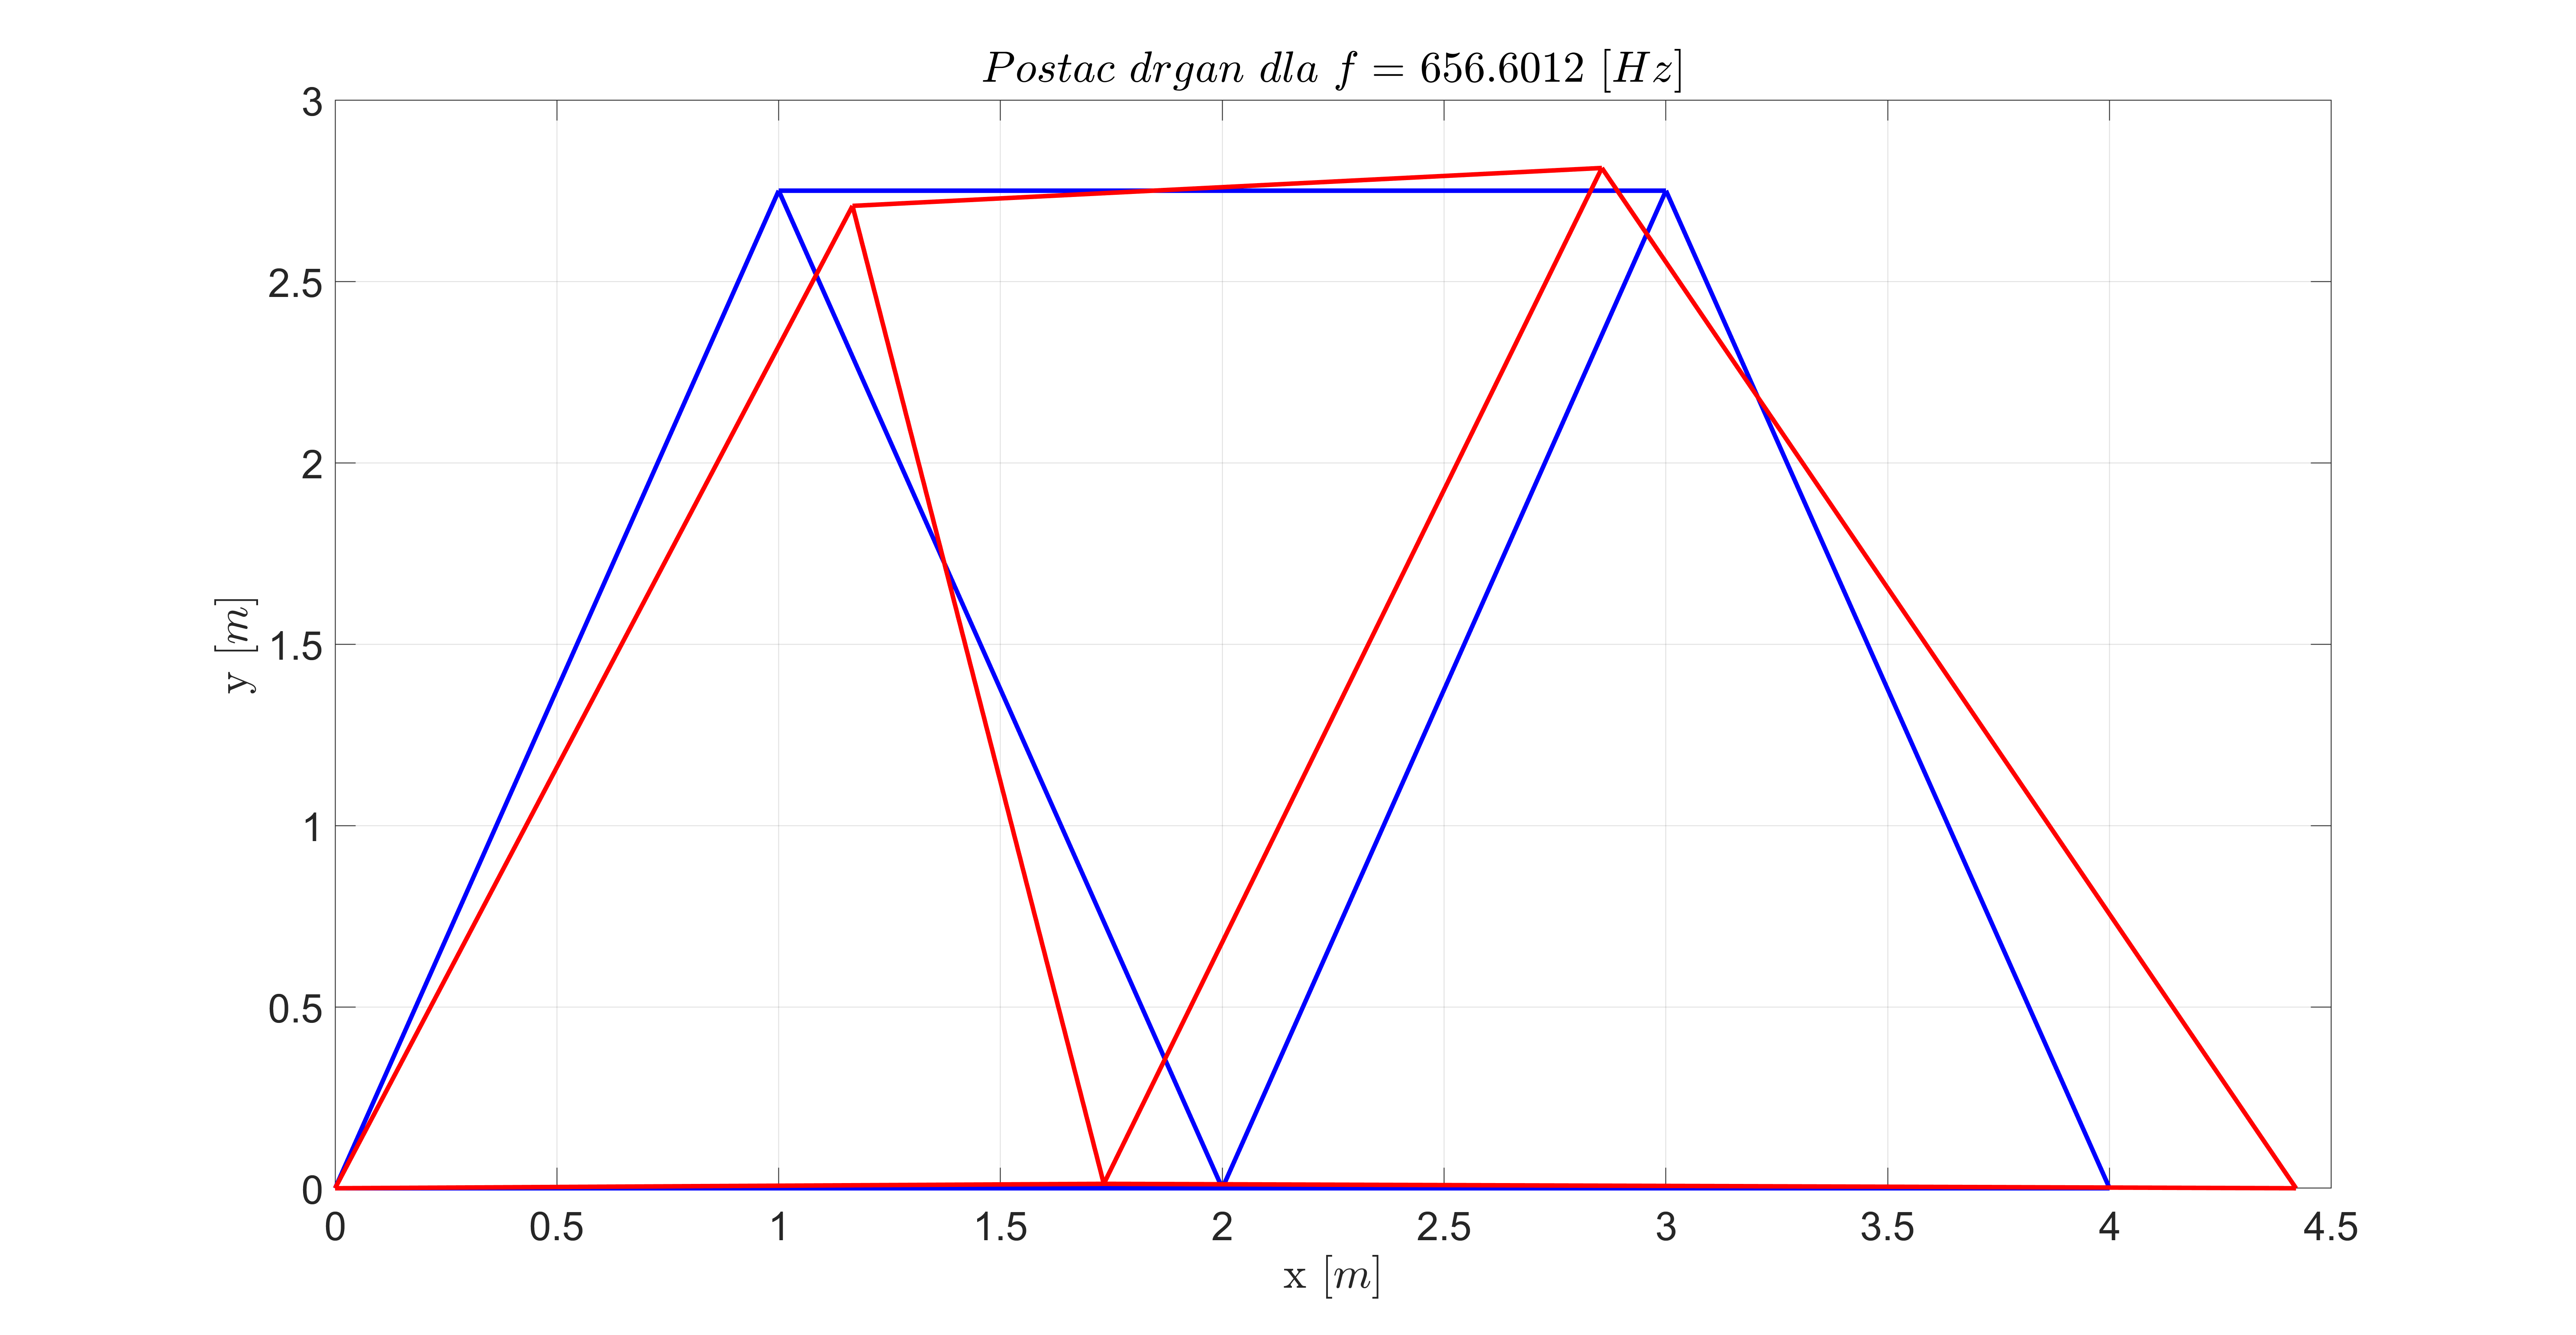
\includegraphics[width=\textwidth, height=0.6\textwidth]{postac_dragn_7.png}
    \caption{Kształt siódmej postaci dragń}
    \label{postac7}
\end{figure}

%%%%%%%%%%%%%%%%%%%%%%%%%%%%%%%%%%%%%%%%%%%%%%%%%%%%%%%%%%%%%%%%%%%%%%%%%%%%%%%%%%%%%
\section{Kratownica - rozwiązanie w środowisku ANSYS Workbench}
\label{sec:work}

W celu weryfikacji wyników otrzymanych w środowisku Matlab została przeprowadzona symulacja w środowisku ANSYS Workbench będącym zaawansowanym narzędziem CAE.

W środowisku tym stworzony został model geometryczny, który widoczny jest na rysunku \ref{rys:modelsiatki}. Model ten posiada wszsytkie parametry (geometryczne, materiałowe itp.) takie jak model stworzony w rozdziale \ref{sec:matlab}. Przyjęto także okrągły przekrój kratownicy o promieniu dobranym na podstawie zgodności pól przekroju.

%%%%%%%%%%%%%%%%%%%%%%%%%%%%%
\subsection{Analiza statyczna}
\label{sec:ansys:statyczna}

W celu sprawdzenia analizy statycznej z rodziału \ref{sec:stat:matlab} model geometryczny został podzielony na elementy skończone. Za element skończony został przyjęty model elementu \textit{LINK 180}. Na rys \ref{rys:modelsiatki} widoczna jest siatka elementów skończonych. Jak widać dobrany zotał 1 element skończony na długość każdego pręta kratownicy. Pozowli to uzyskać zbliżone warunki symulacji względem symulacji dokonanej w Matlabie, gdzie każdy pręt był jednym elementem.

Nastepnie zastosowano warunki brzegowe w postaci siły skupionej oraz utwierdzenia odpowiednich węzłów. Warunki te widoczne są na rysunku \ref{rys:warunkibrzegowe}.

\newpage

\begin{figure}[H]
    \centering
    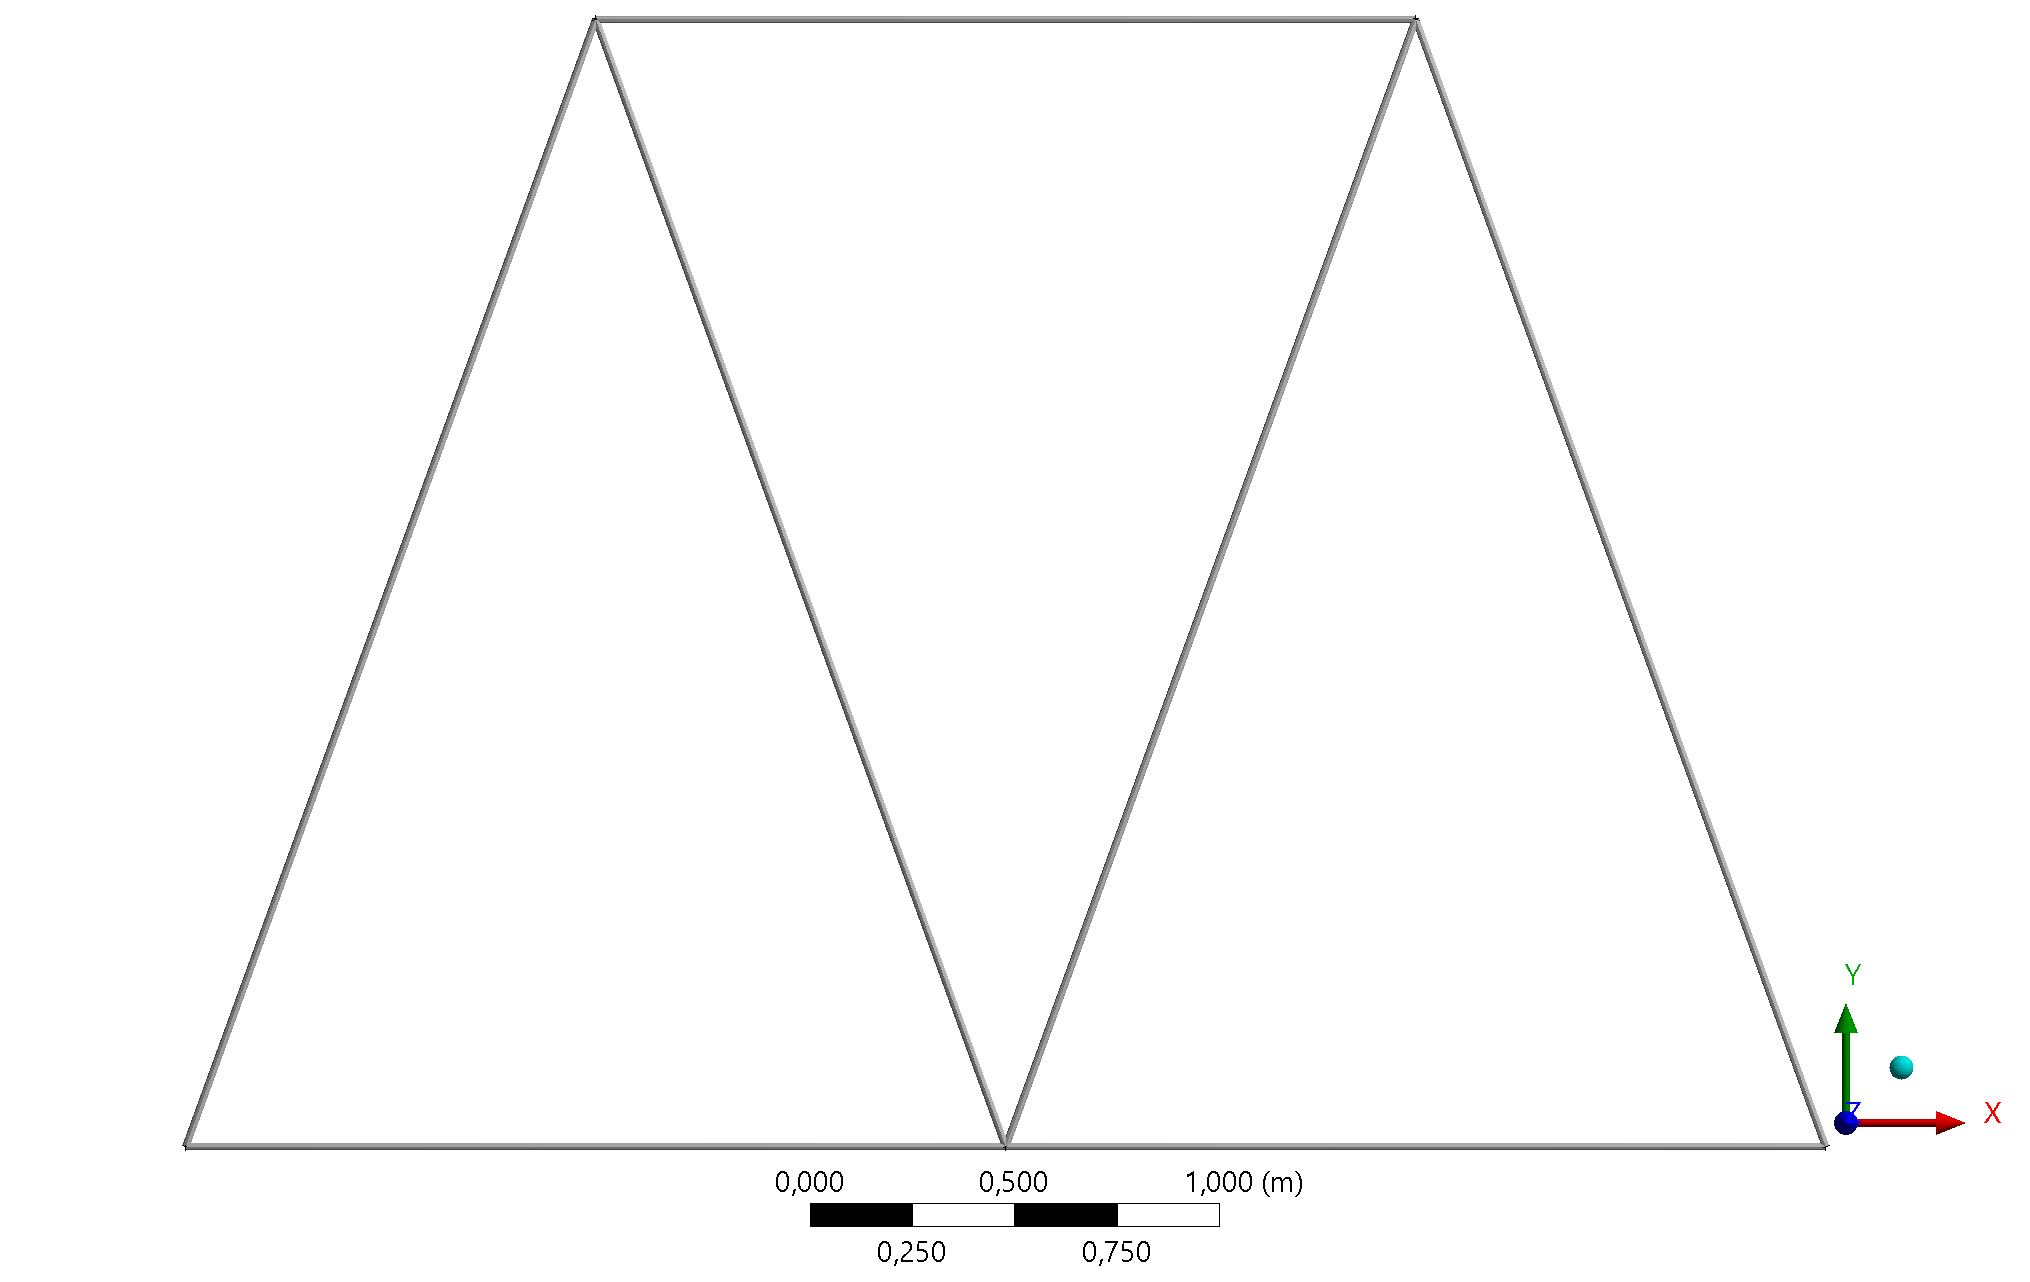
\includegraphics[width=\textwidth, height=0.6\textwidth]{ModelgeomZSiatka.png}
    \caption{Siatka elementów skończonych}
    \label{rys:modelsiatki}
\end{figure}


\begin{figure}[H]
    \centering
    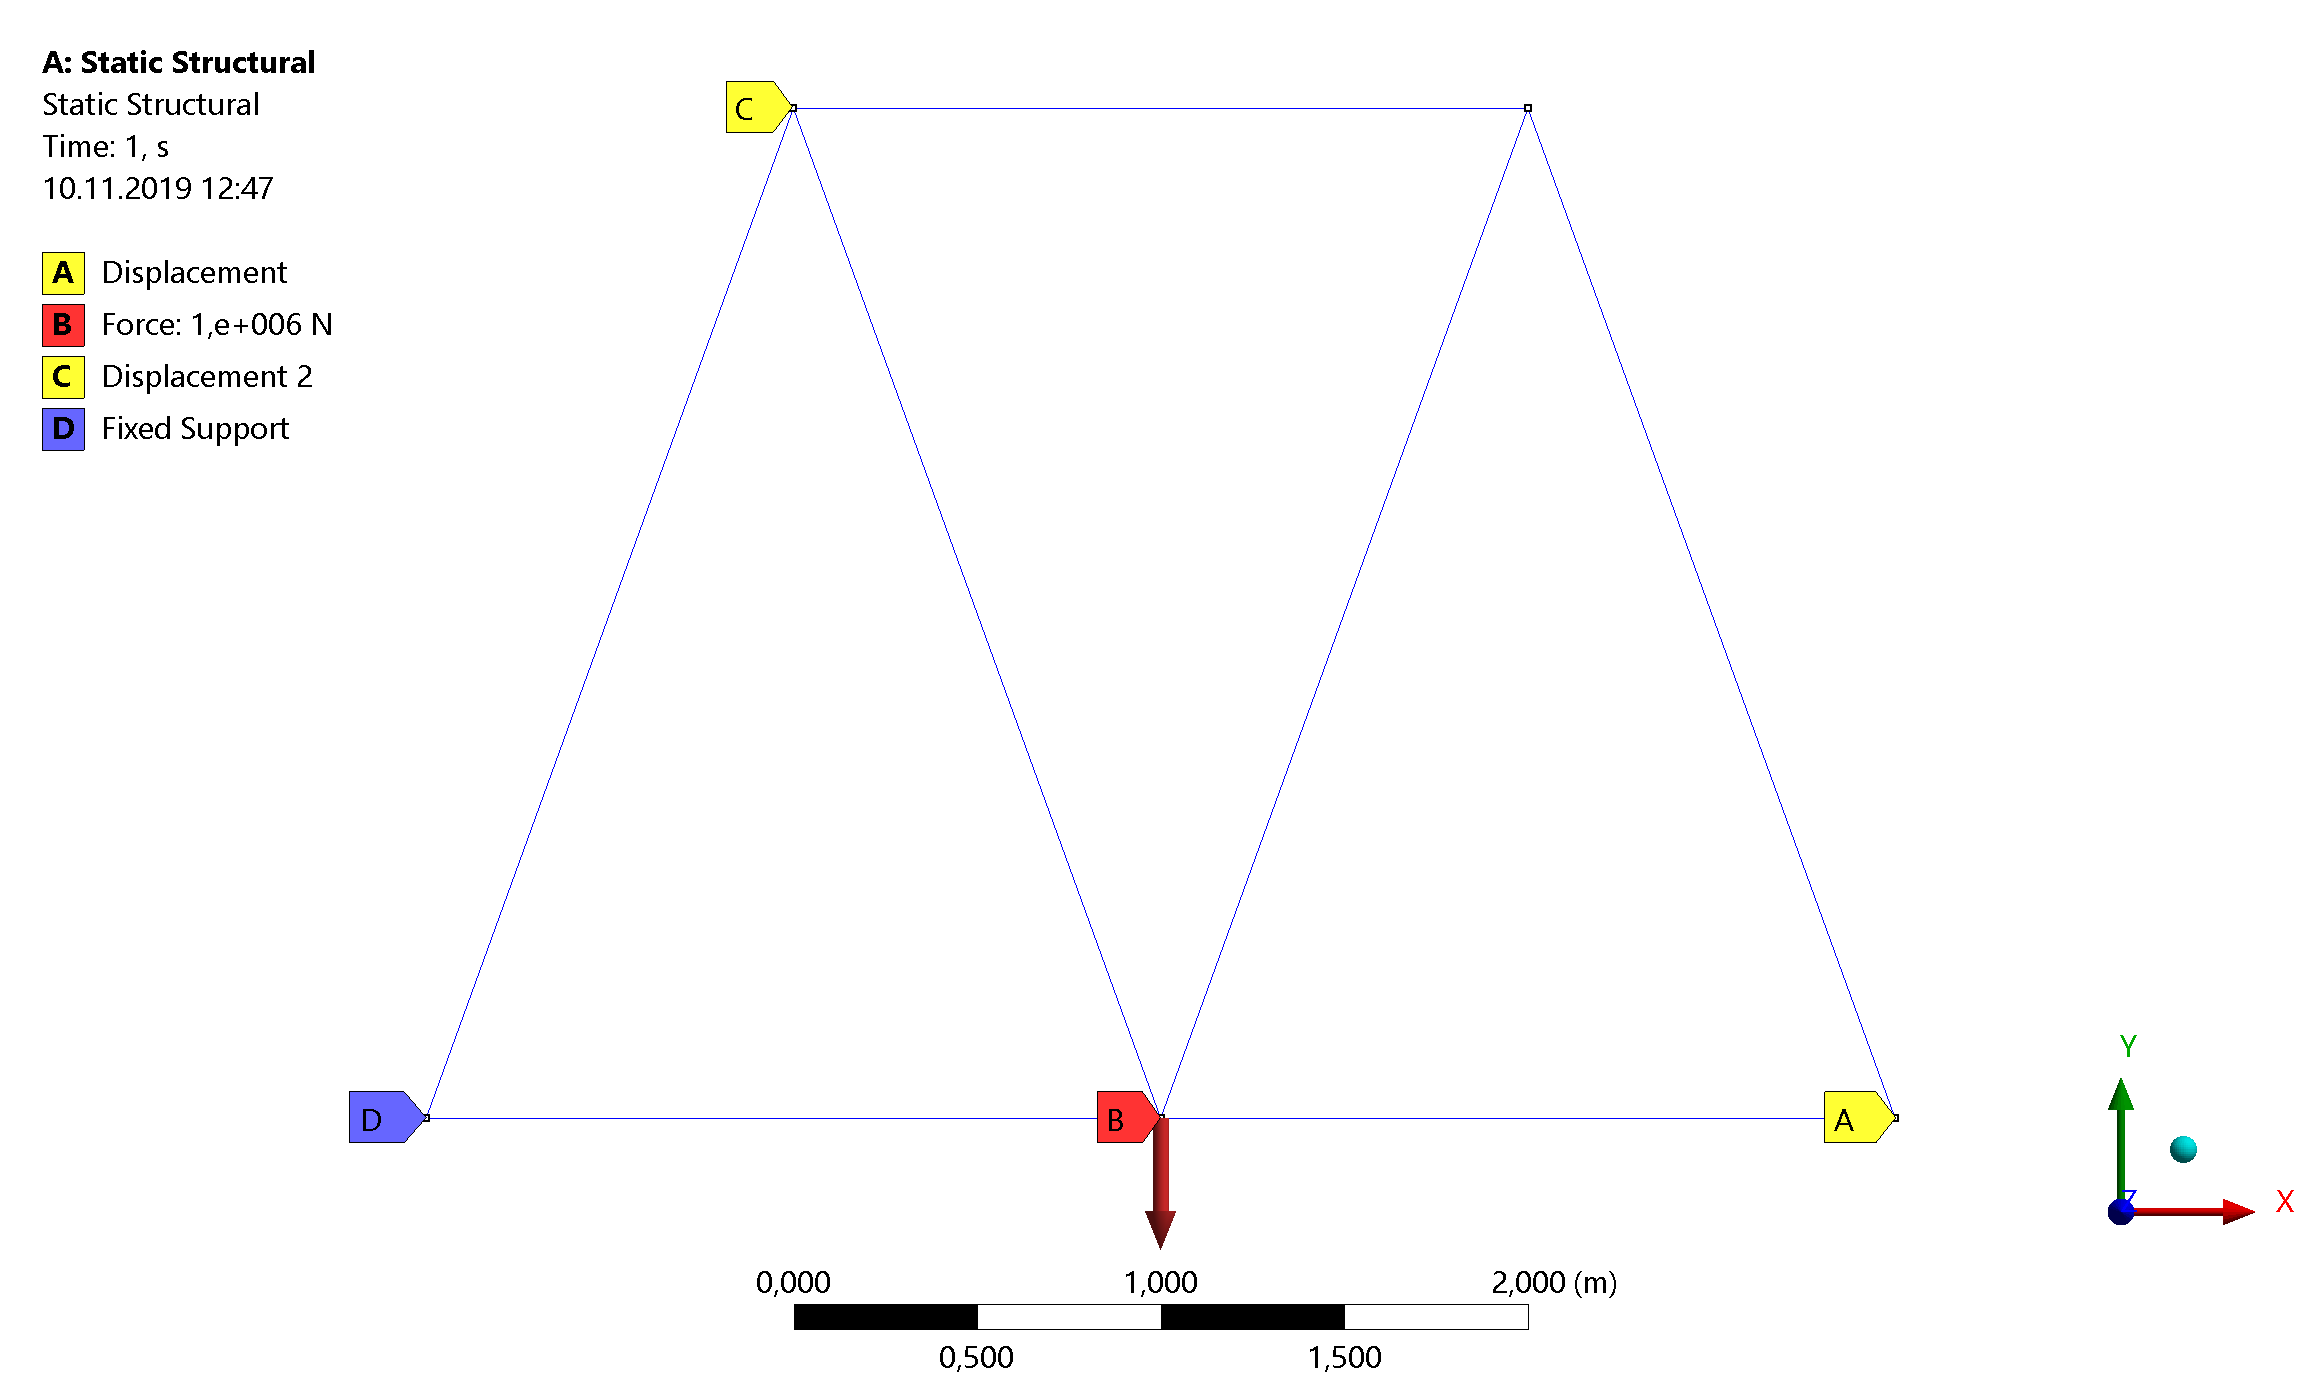
\includegraphics[width=\textwidth, height=0.6\textwidth]{StructuralSettings.png}
    \caption{Warunki brzegowe dla analizy statycznej}
    \label{rys:warunkibrzegowe}
\end{figure}

Po wykonaniu obliczeń uzyskane wyniki zostały przedstawione na rysunkach poniżej. Przedstawione zostaną przemieszczenia węzłowe konstrukcji w celu porównania z wynikami obliczeń w środowkisku Matlab.

\begin{figure}[H]
    \centering
    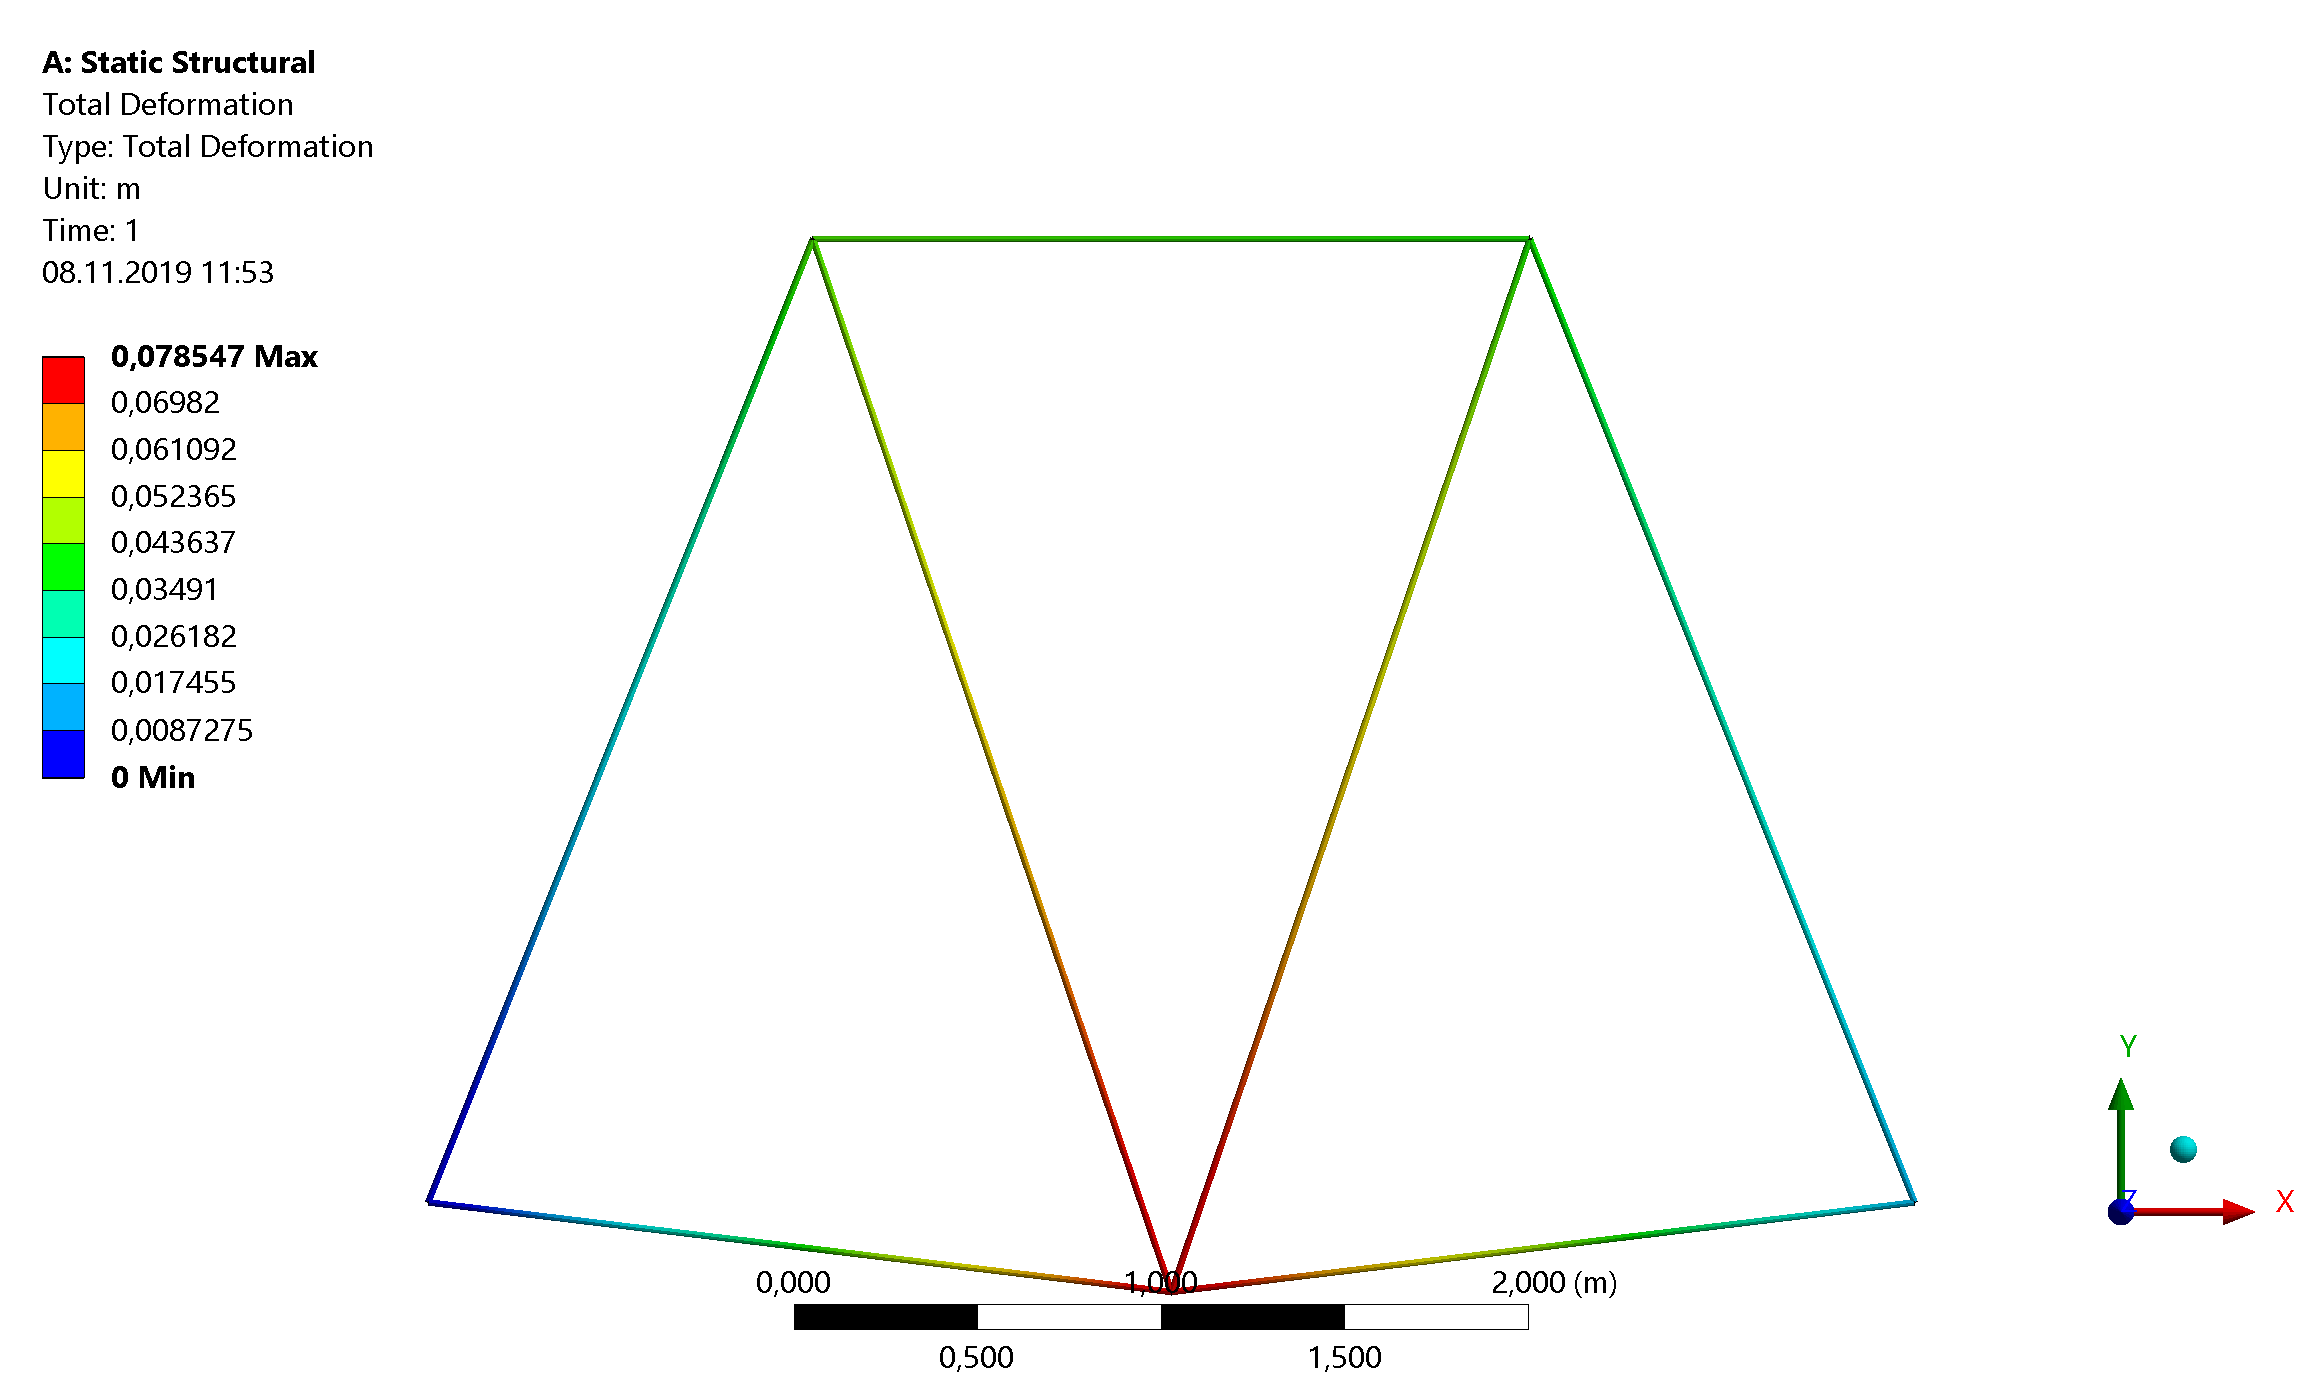
\includegraphics[width=\textwidth, height=0.55\textwidth]{StructuralTotalDef.png}
    \caption{Odkształcenia całkowite kratownicy}
    \label{rys:totaldef}
\end{figure}

\begin{figure}[H]
    \centering
    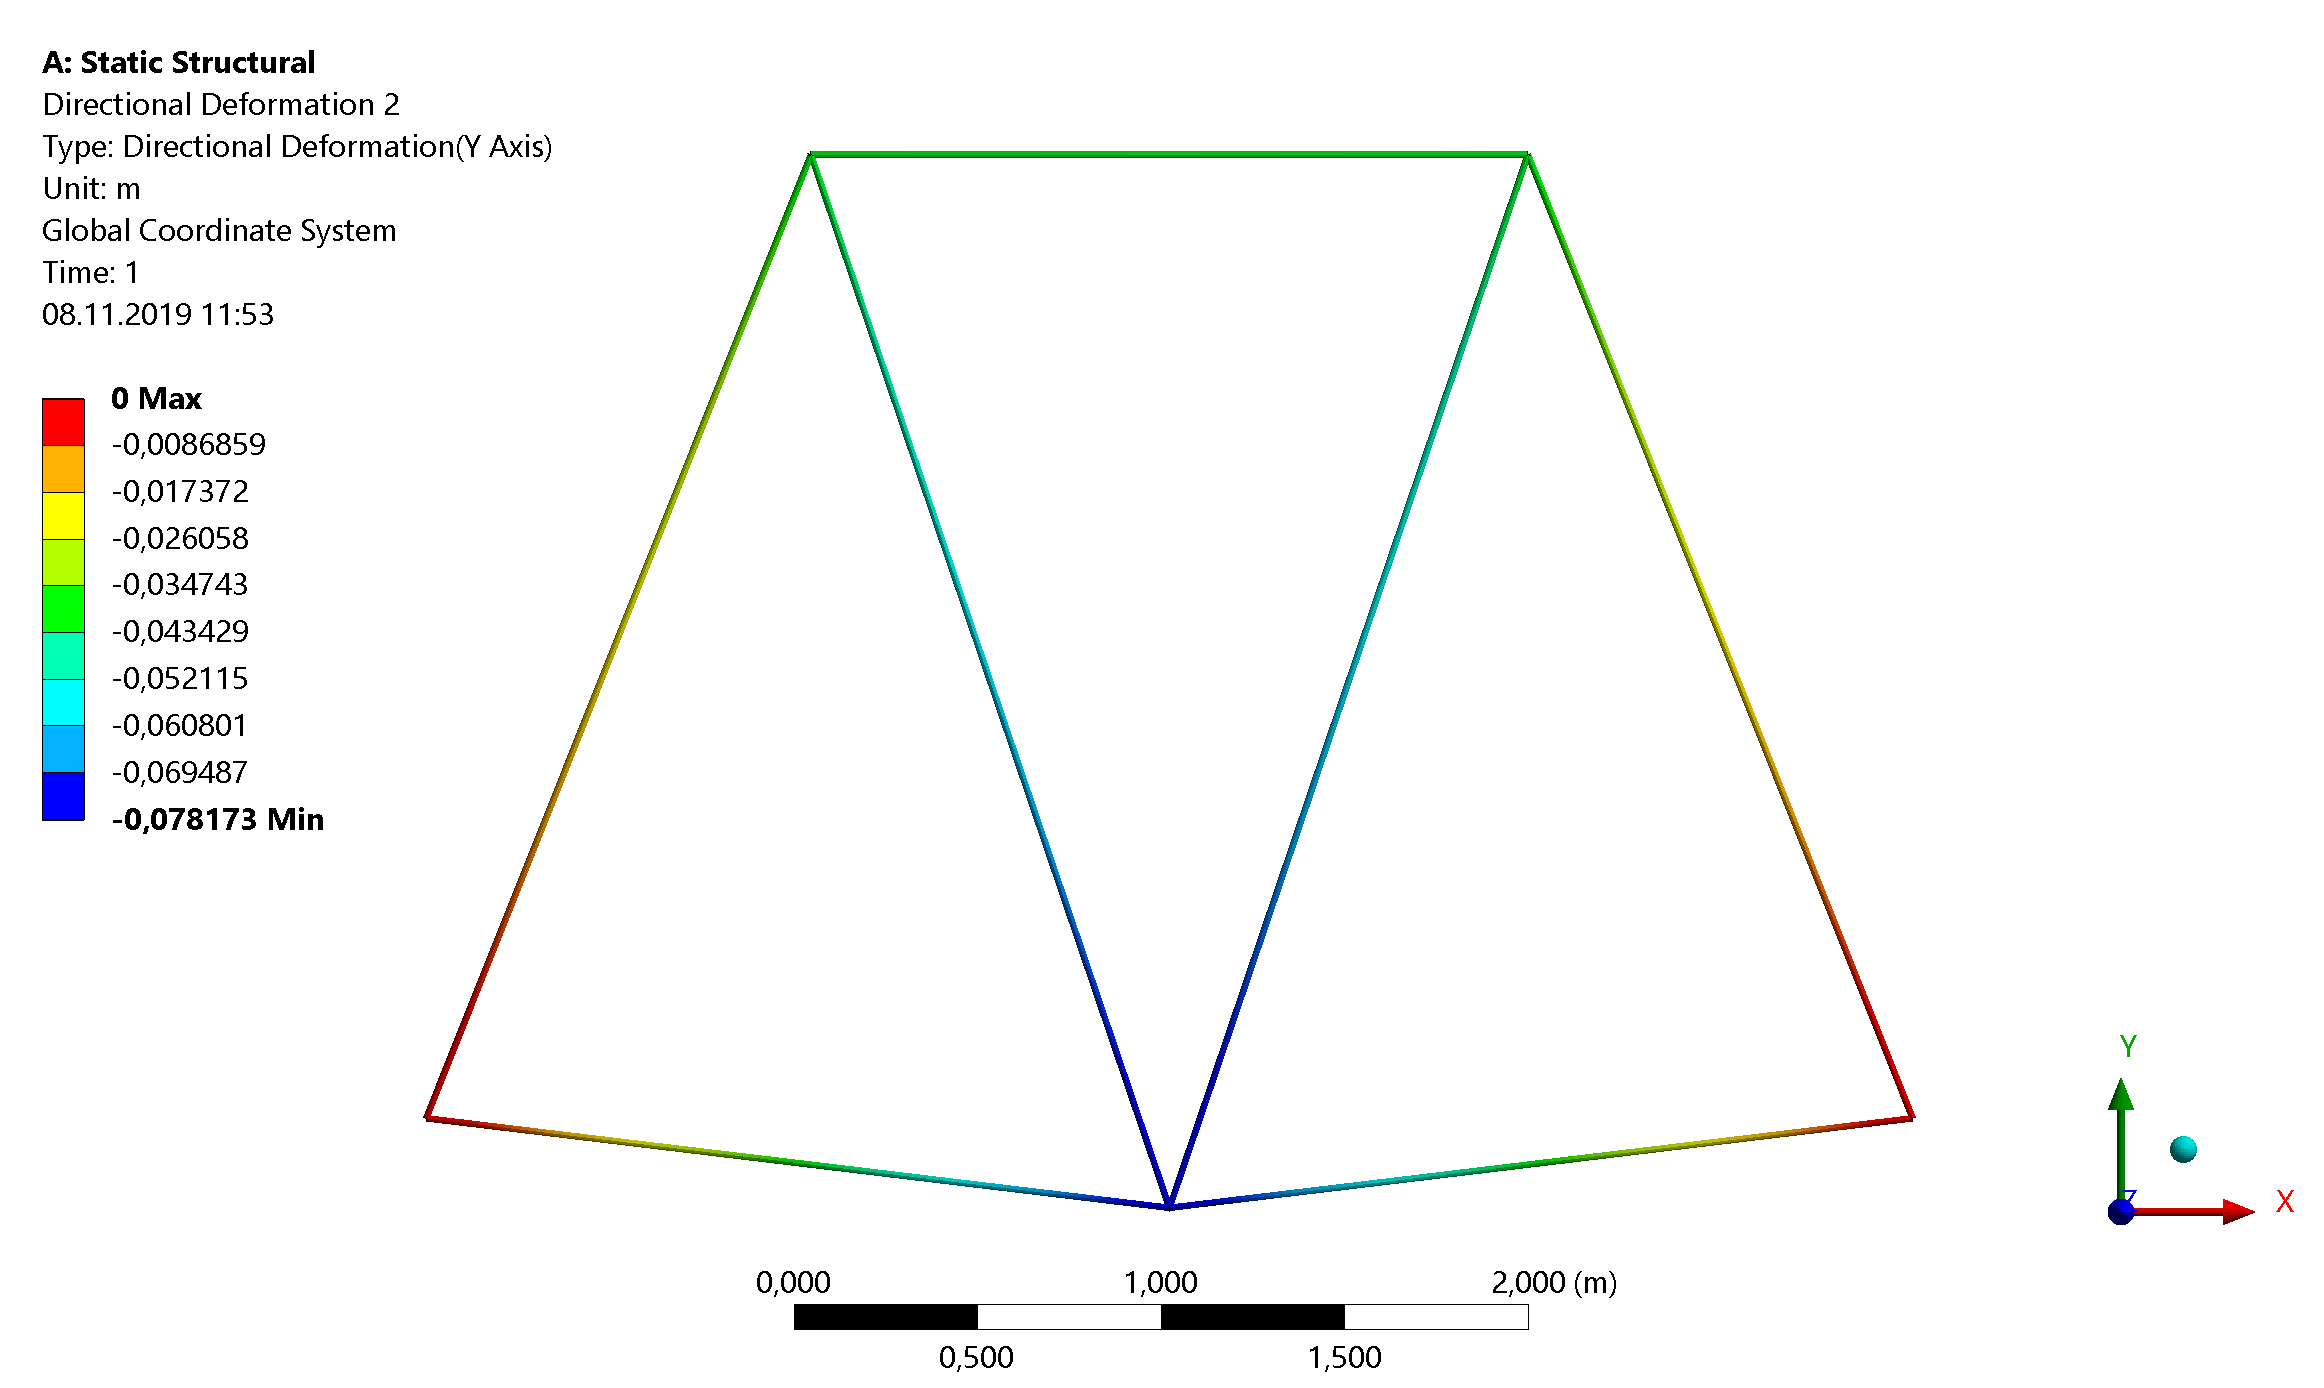
\includegraphics[width=\textwidth, height=0.55\textwidth]{StructuralYDef.png}
    \caption{Odkształcenia na kierunku pionowym (Y) kratownicy}
    \label{rys:ydef}
\end{figure}



\subsection{Analiza dynamicza}
\label{sec:ansys:dynamiczna}

Analize modalną kratownicy w środowisku ANSYS Workbench dokonano na podstawie modelu geometrycznego pokazanego w rodziale \ref{sec:work}. Przyjęte warunki brzegowe zostały przedstawione na rysunku  \ref{rys:warbrzegmodal}. Zostały zastosowane utwierdzenia odpowiadające podporom z kratownicy jak w punkcie \ref{sec:matlab}. Dodatkowo odebrane zostały stopnie swobody na kierunku prostopadłym do płaszczyzny modelu we wszsytkich węzłach konstrukcji.

\begin{figure}[H]
    \centering
    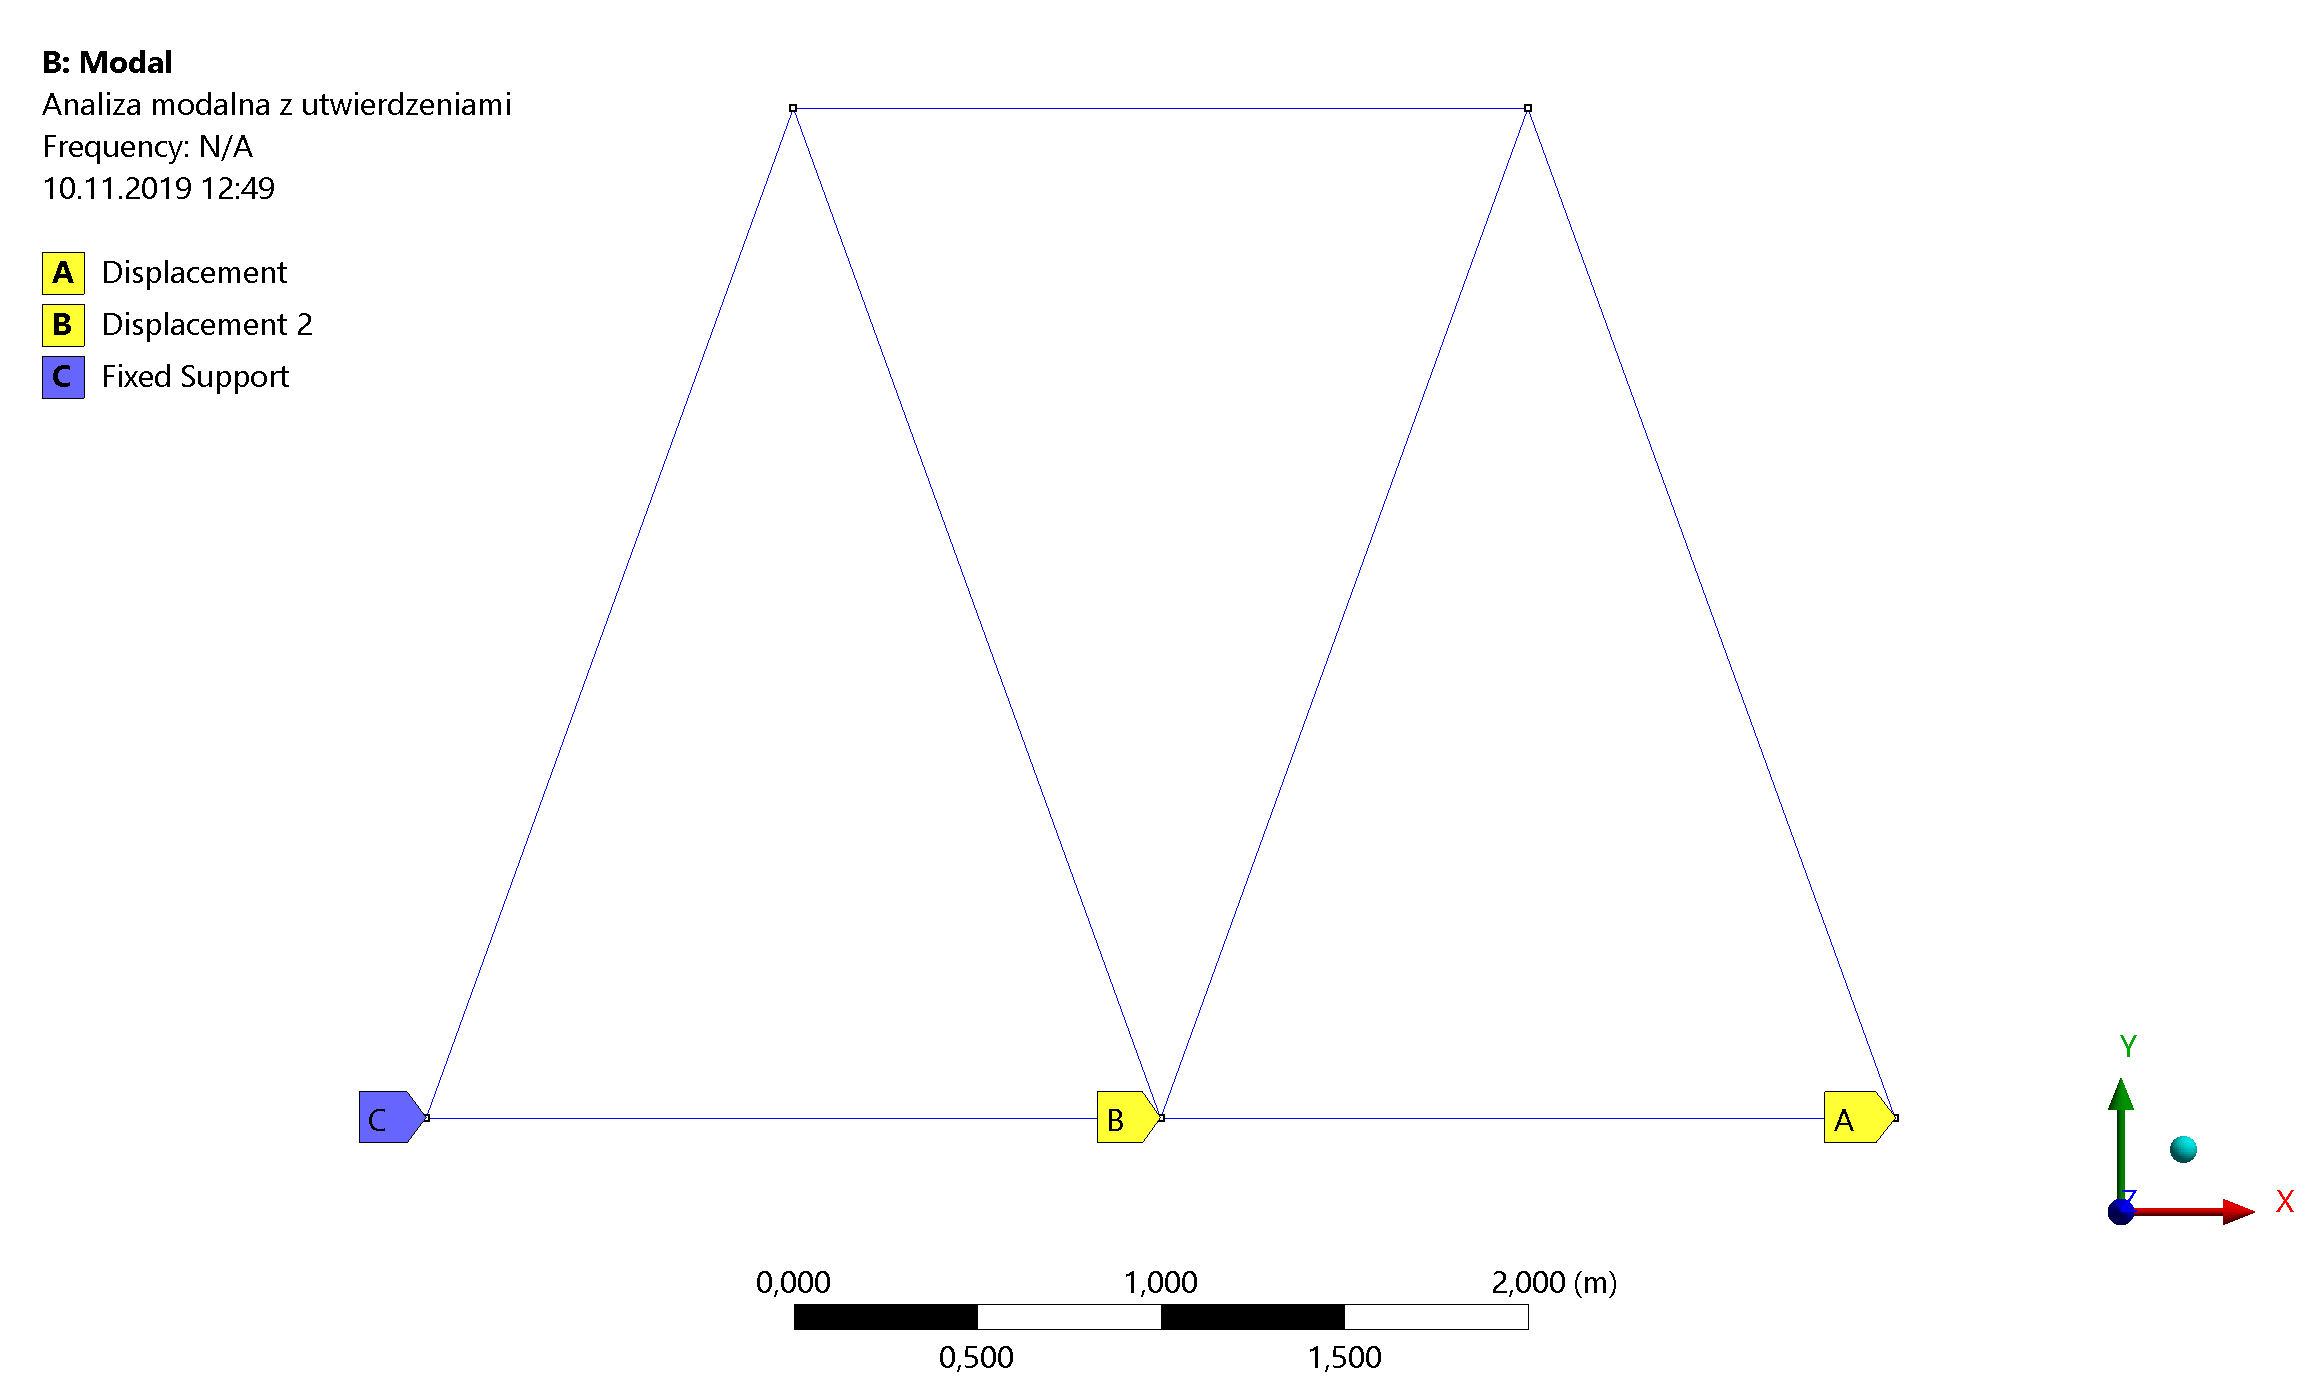
\includegraphics[width=\textwidth, height=0.6\textwidth]{modalsettings.png}
    \caption{Warunki brzegowe do analizy modalnej}
    \label{rys:warbrzegmodal}
\end{figure}

Otrzymane w wyniku analizy modalnej częstości drgań widoczne są w poniższej tabeli. Wyniki idealnie pokrywają się z wynikami uzyskanymi w środowisku Matlab, pod warunkiem zastosowania odpowiednich utwierdzeń oraz elementu typu LINK 180. W przypadku elementu domyślego programu ANSYS częstości drgań nie pokrywały się w ogóle. Poniżej znajdują się wyniki w formie tabeli \ref{tab:czestansys} oraz rysunków postaci drgań.

\begin{table}[H]
    \caption{Częstotliwości drgań własnych konstrukcji}
    \centering
    \label{tab:czestansys}
    \begin{tabular}{|l|l|}
    \hline
    Postać drgań & Częstotliwość {[}Hz{]} \\ \hline
    1            & 106,02                  \\ \hline
    2            & 159,13                 \\ \hline
    3            & 275,69                 \\ \hline
    4            & 391,49                 \\ \hline
    5            & 494,66                 \\ \hline
    6            & 549,19                 \\ \hline
    7            & 656,60                 \\ \hline
    
    \end{tabular}
\end{table}

\newpage

\begin{figure}[H]
    \centering
    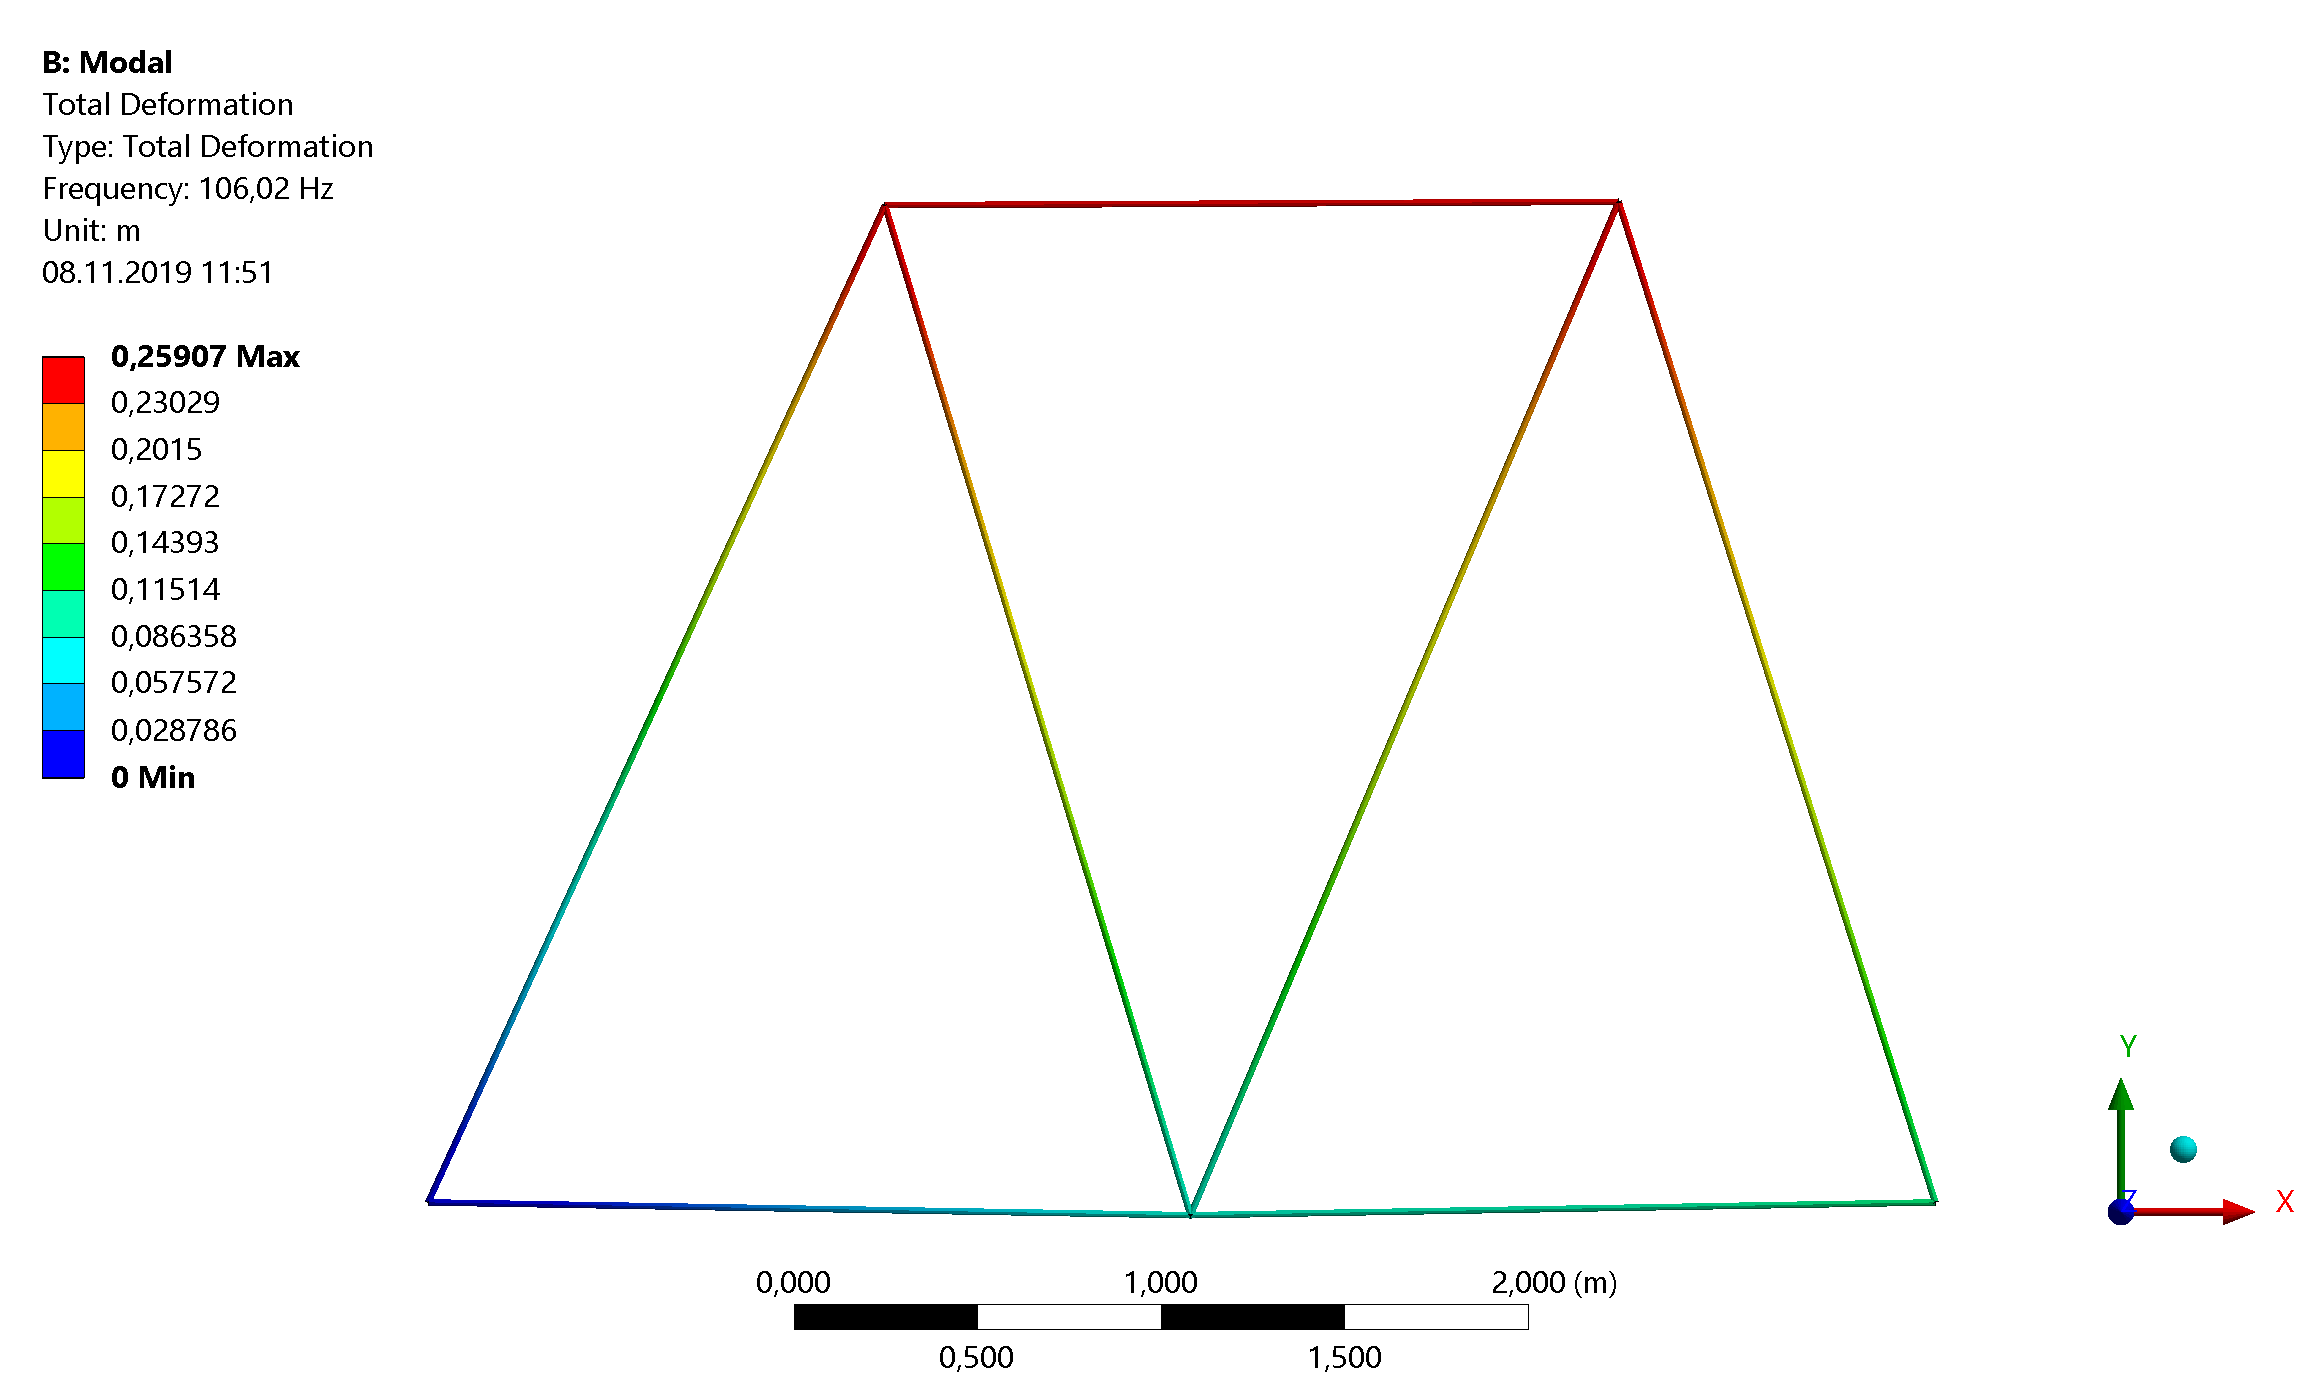
\includegraphics[width=\textwidth, height=0.6\textwidth]{mode1.png}
    \caption{Postać drgań dla $f=106,02\ [Hz]$}
    \label{rys:mode1}
\end{figure}

\begin{figure}[H]
    \centering
    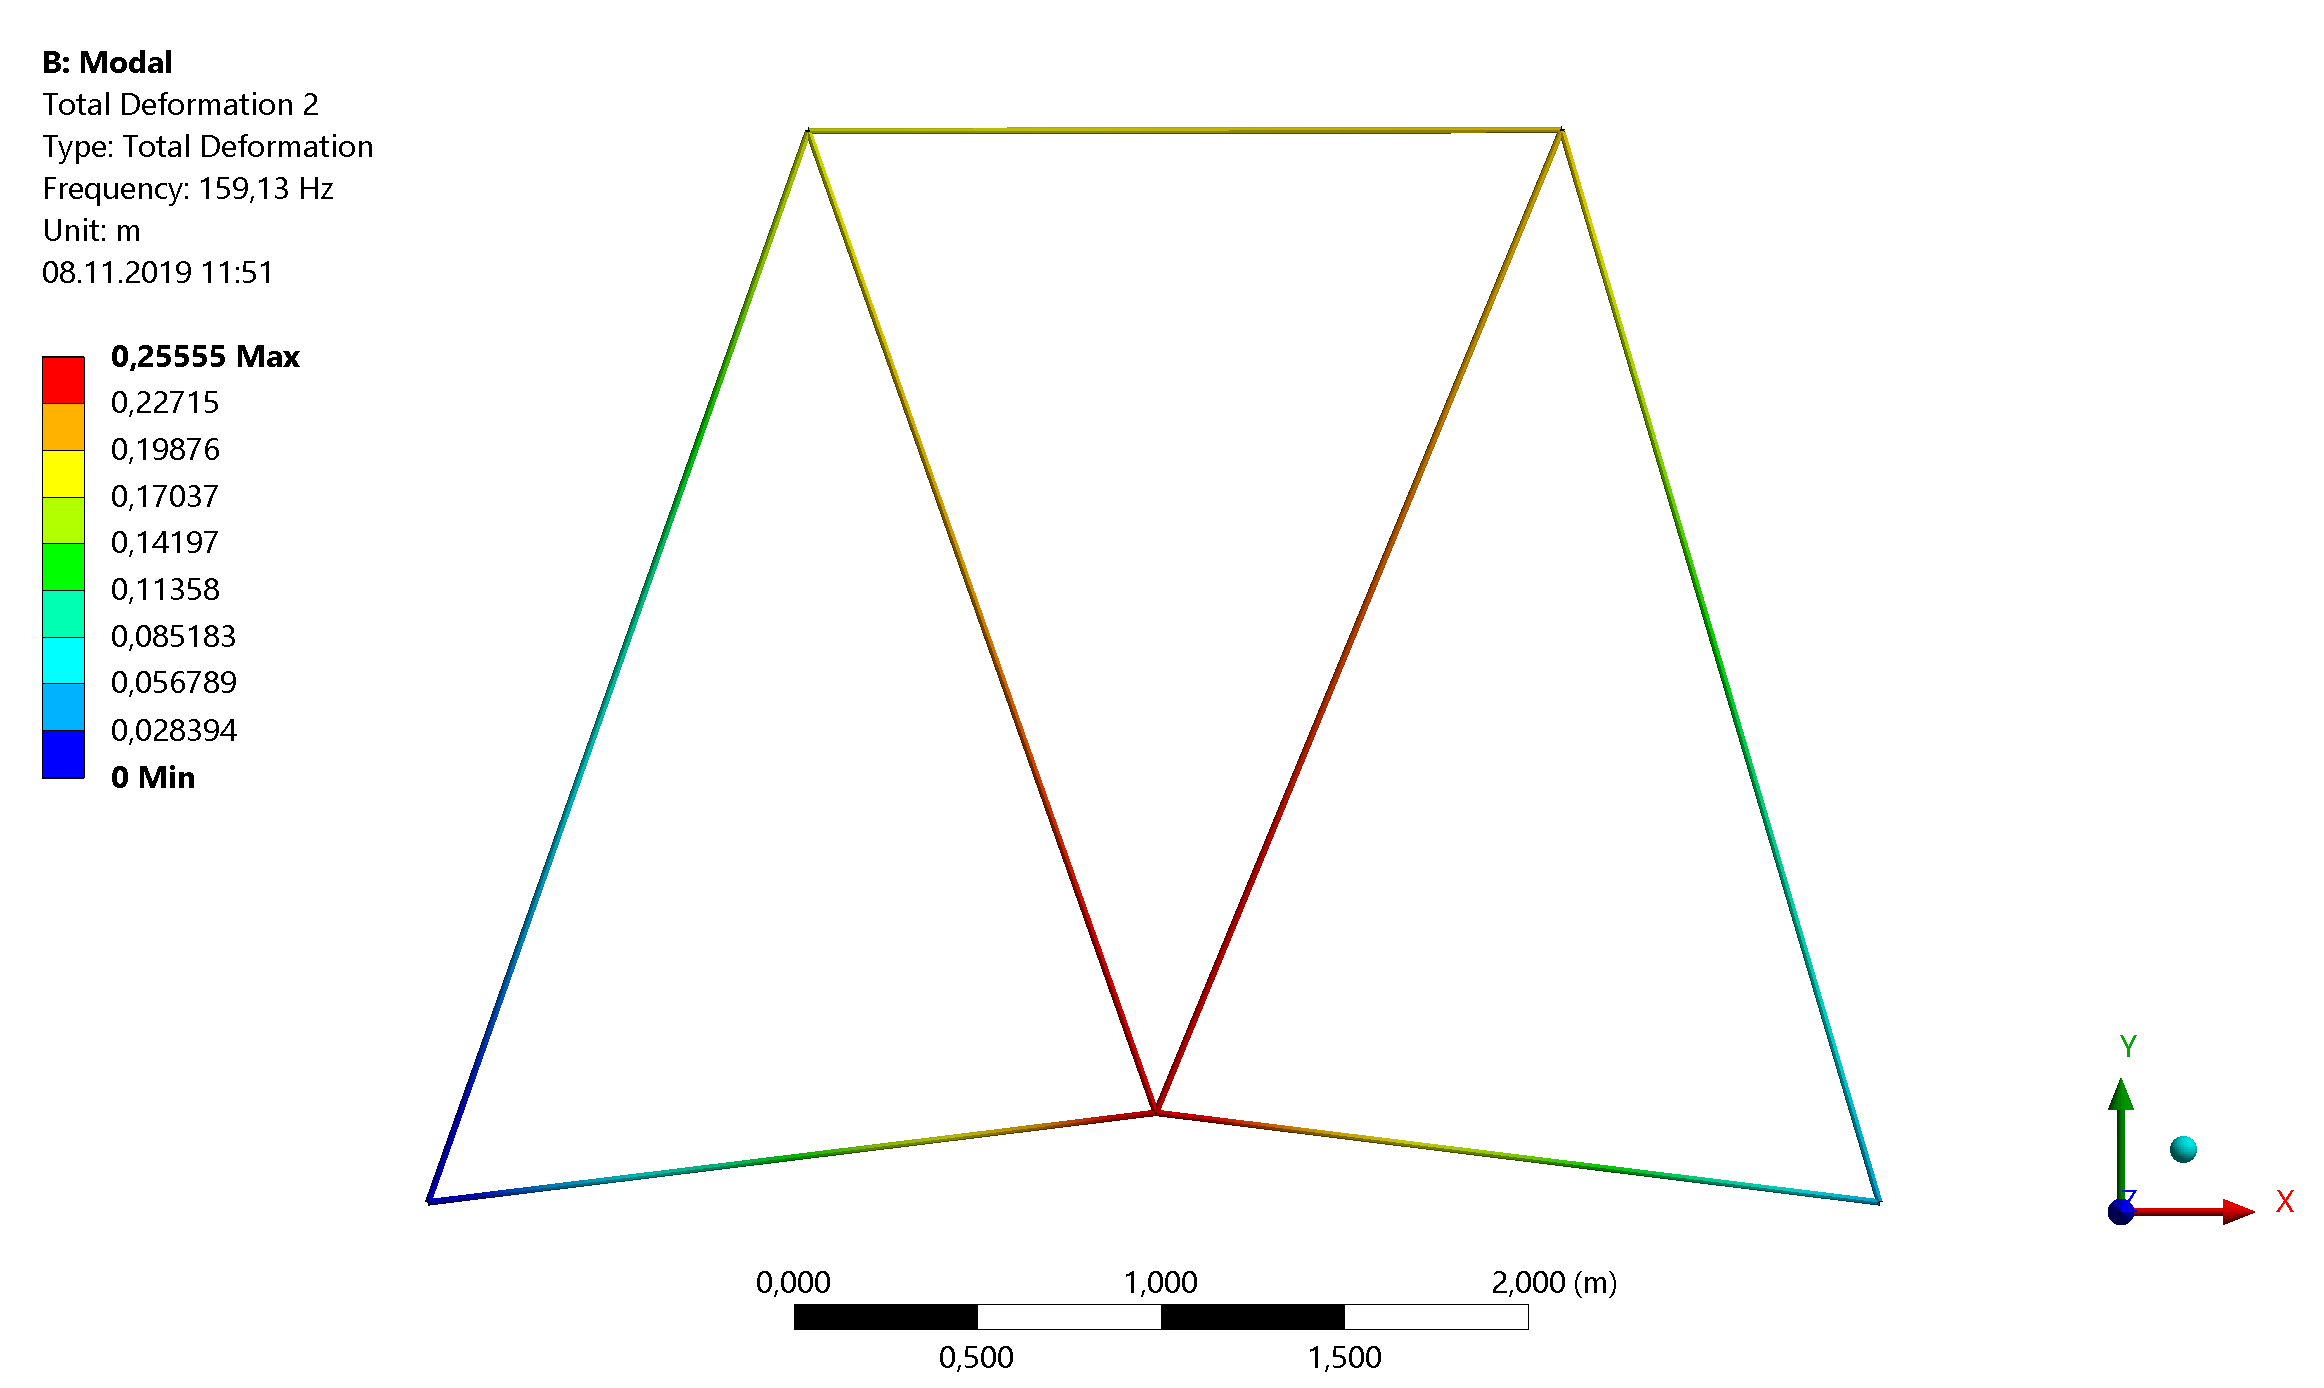
\includegraphics[width=\textwidth, height=0.6\textwidth]{mode2.png}
    \caption{Postać drgań dla $f=159,13\ [Hz]$}
    \label{rys:mode2}
\end{figure}


\begin{figure}[H]
    \centering
    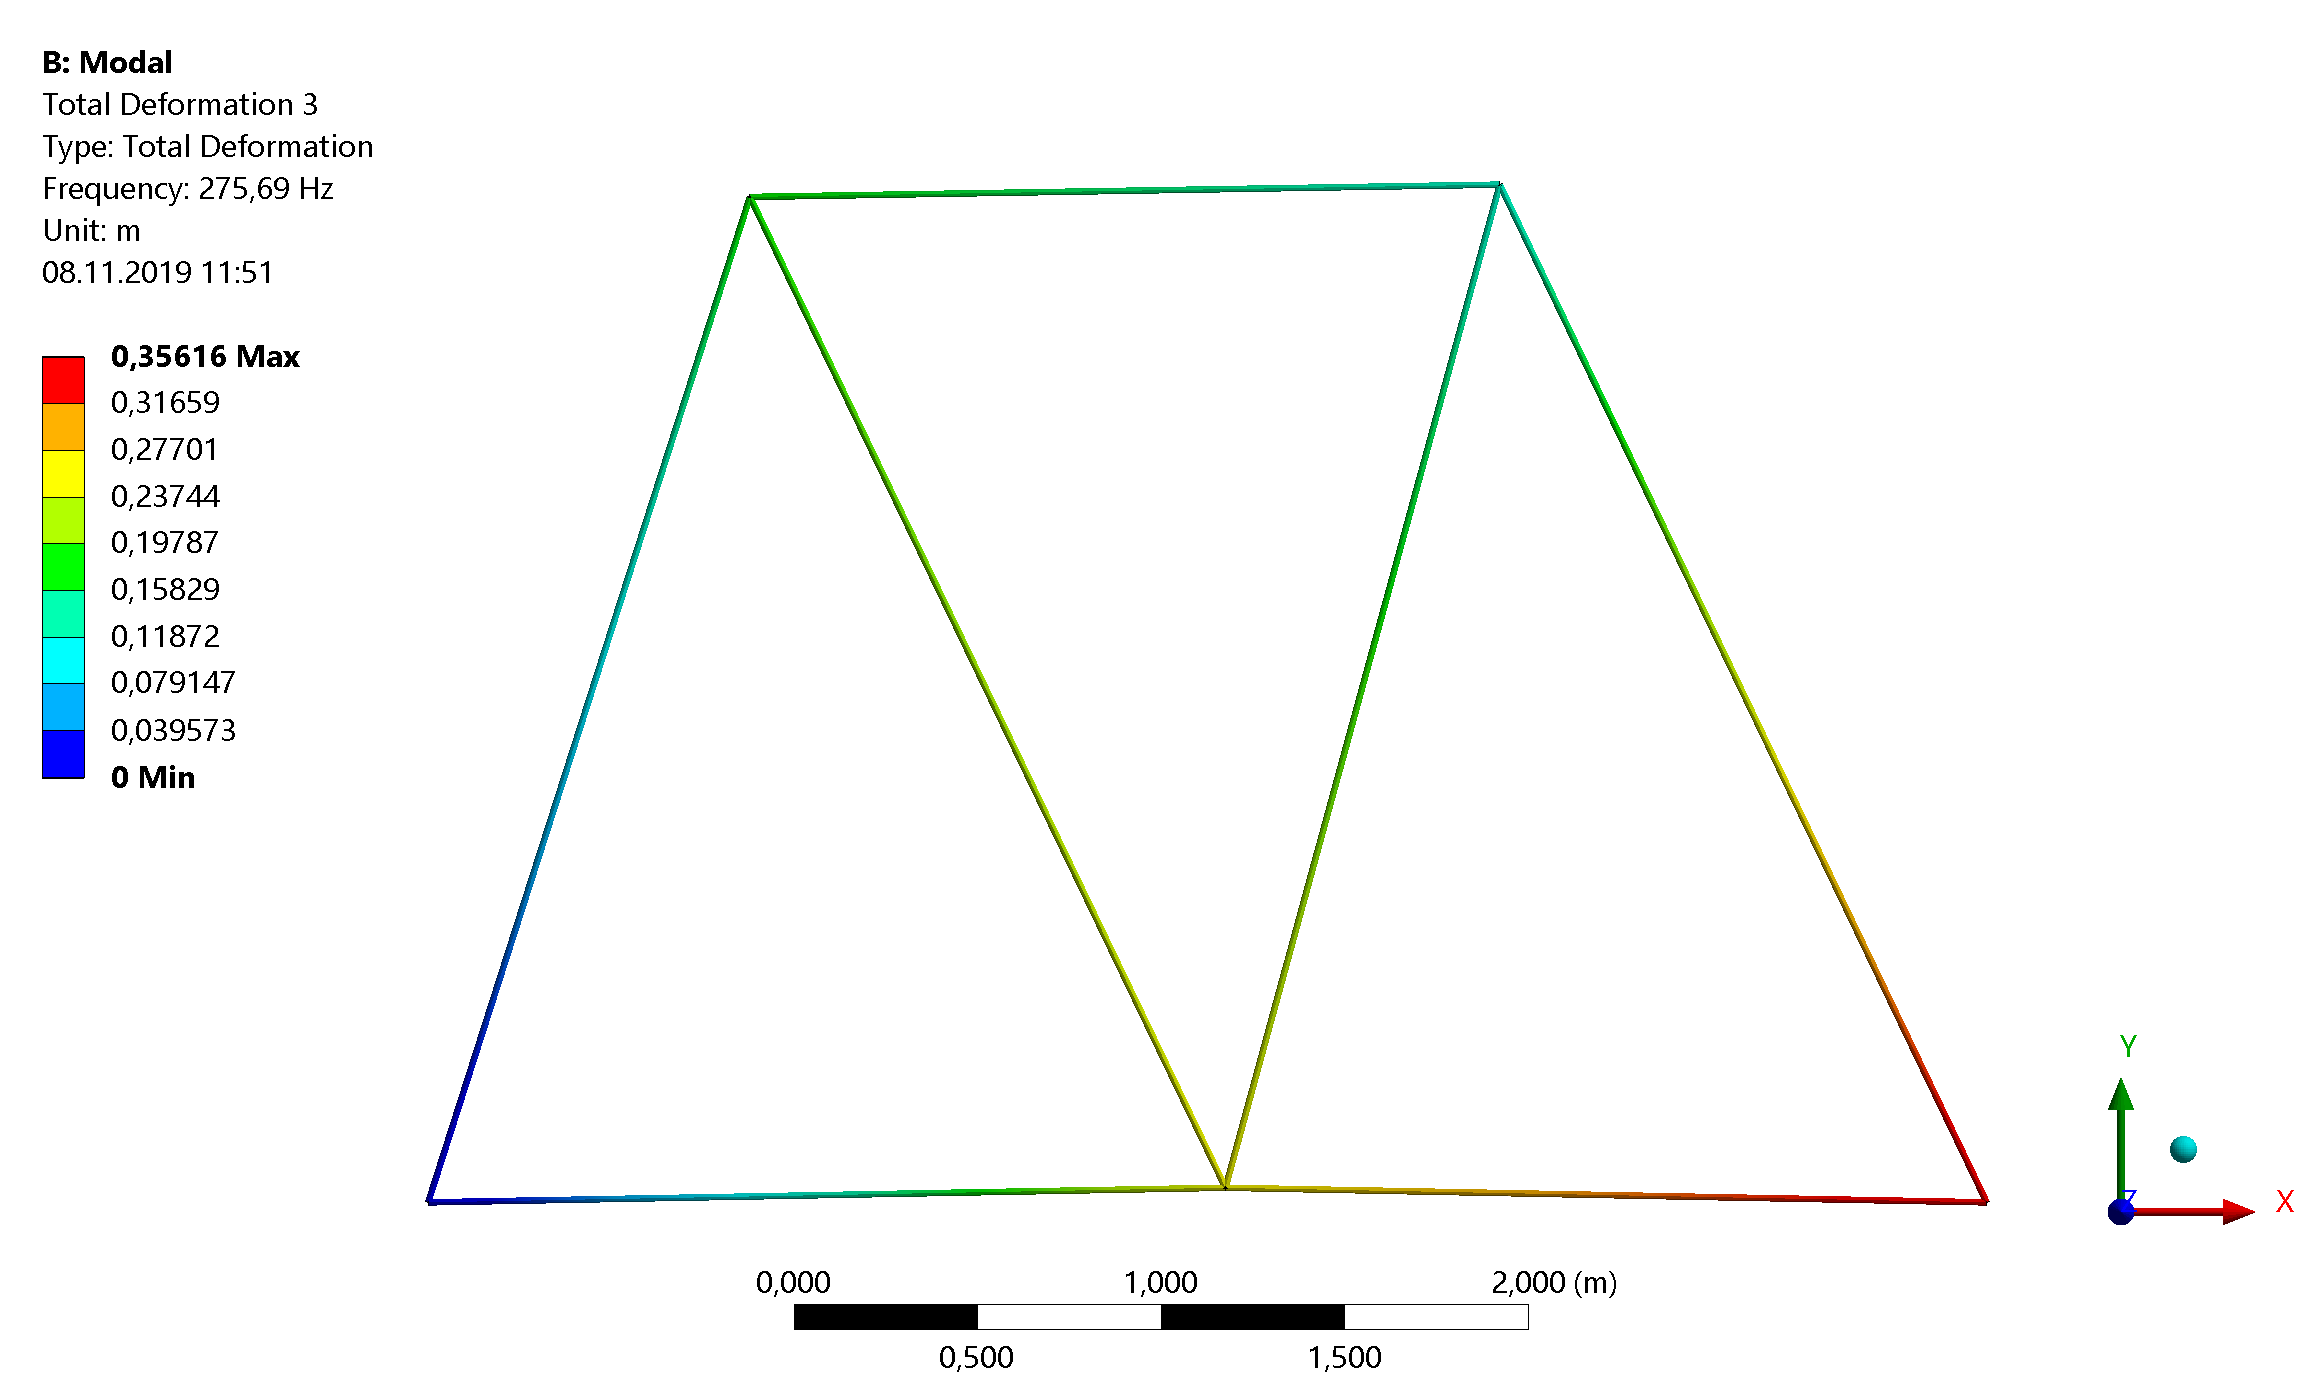
\includegraphics[width=\textwidth, height=0.6\textwidth]{mode3.png}
    \caption{Postać drgań dla $f=275,69\ [Hz]$}
    \label{rys:mode3}
\end{figure}


\begin{figure}[H]
    \centering
    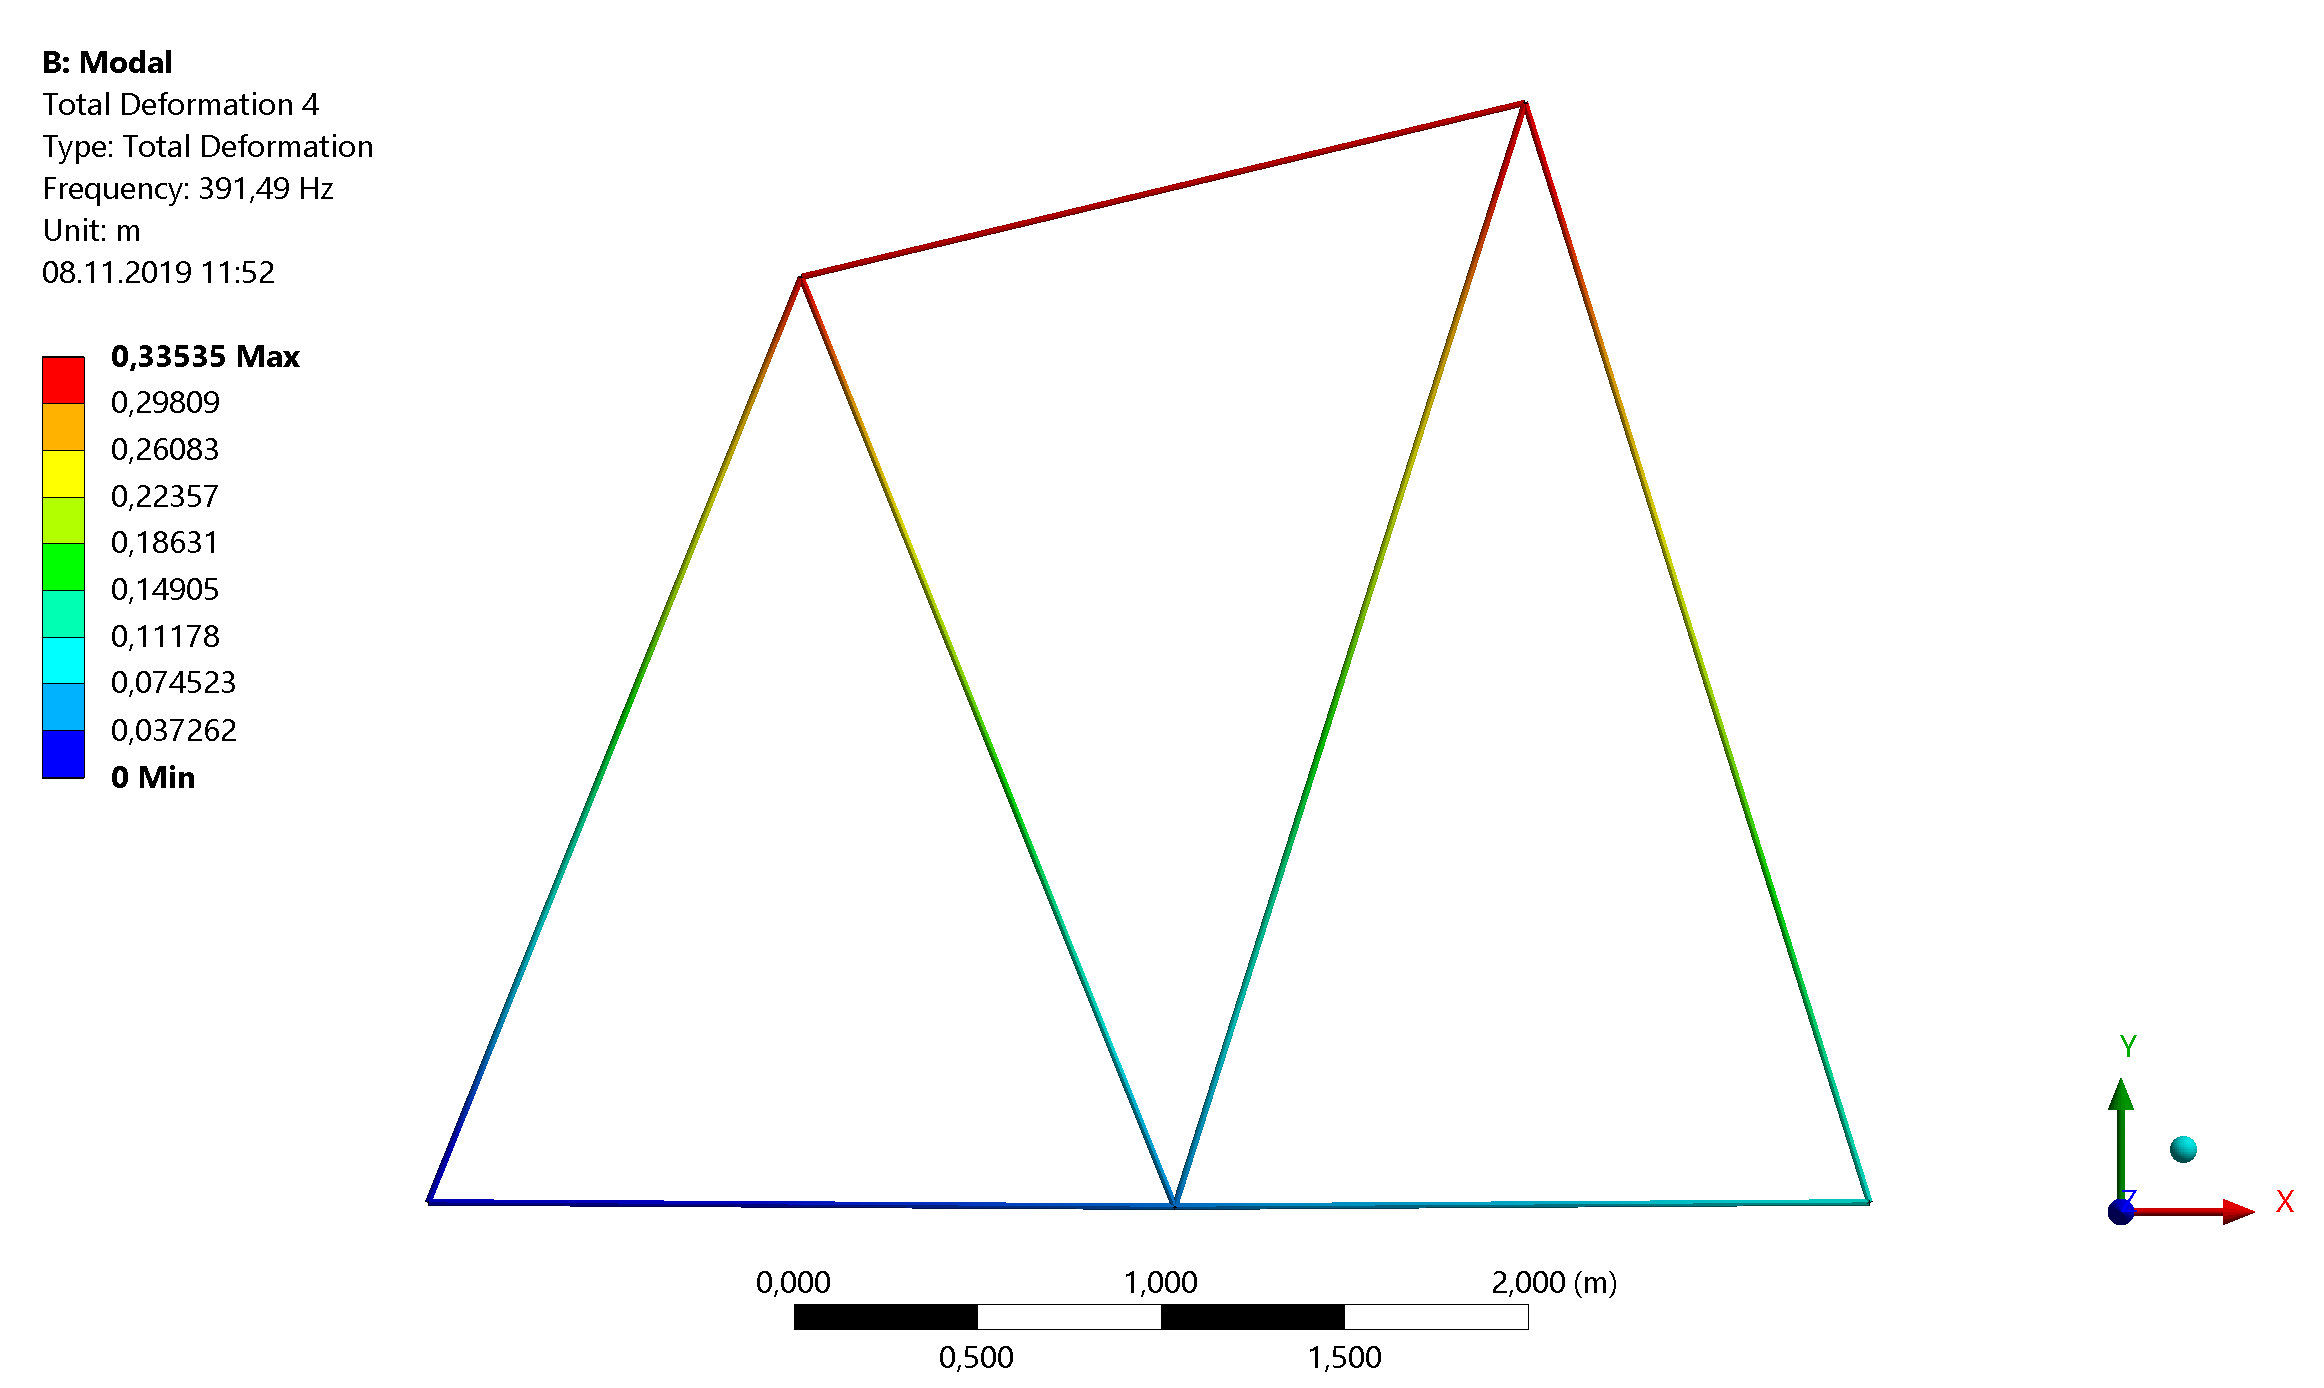
\includegraphics[width=\textwidth, height=0.6\textwidth]{mode4.png}
    \caption{Postać drgań dla $f=391,49\ [Hz]$}
    \label{rys:mode4}
\end{figure}

\begin{figure}[H]
    \centering
    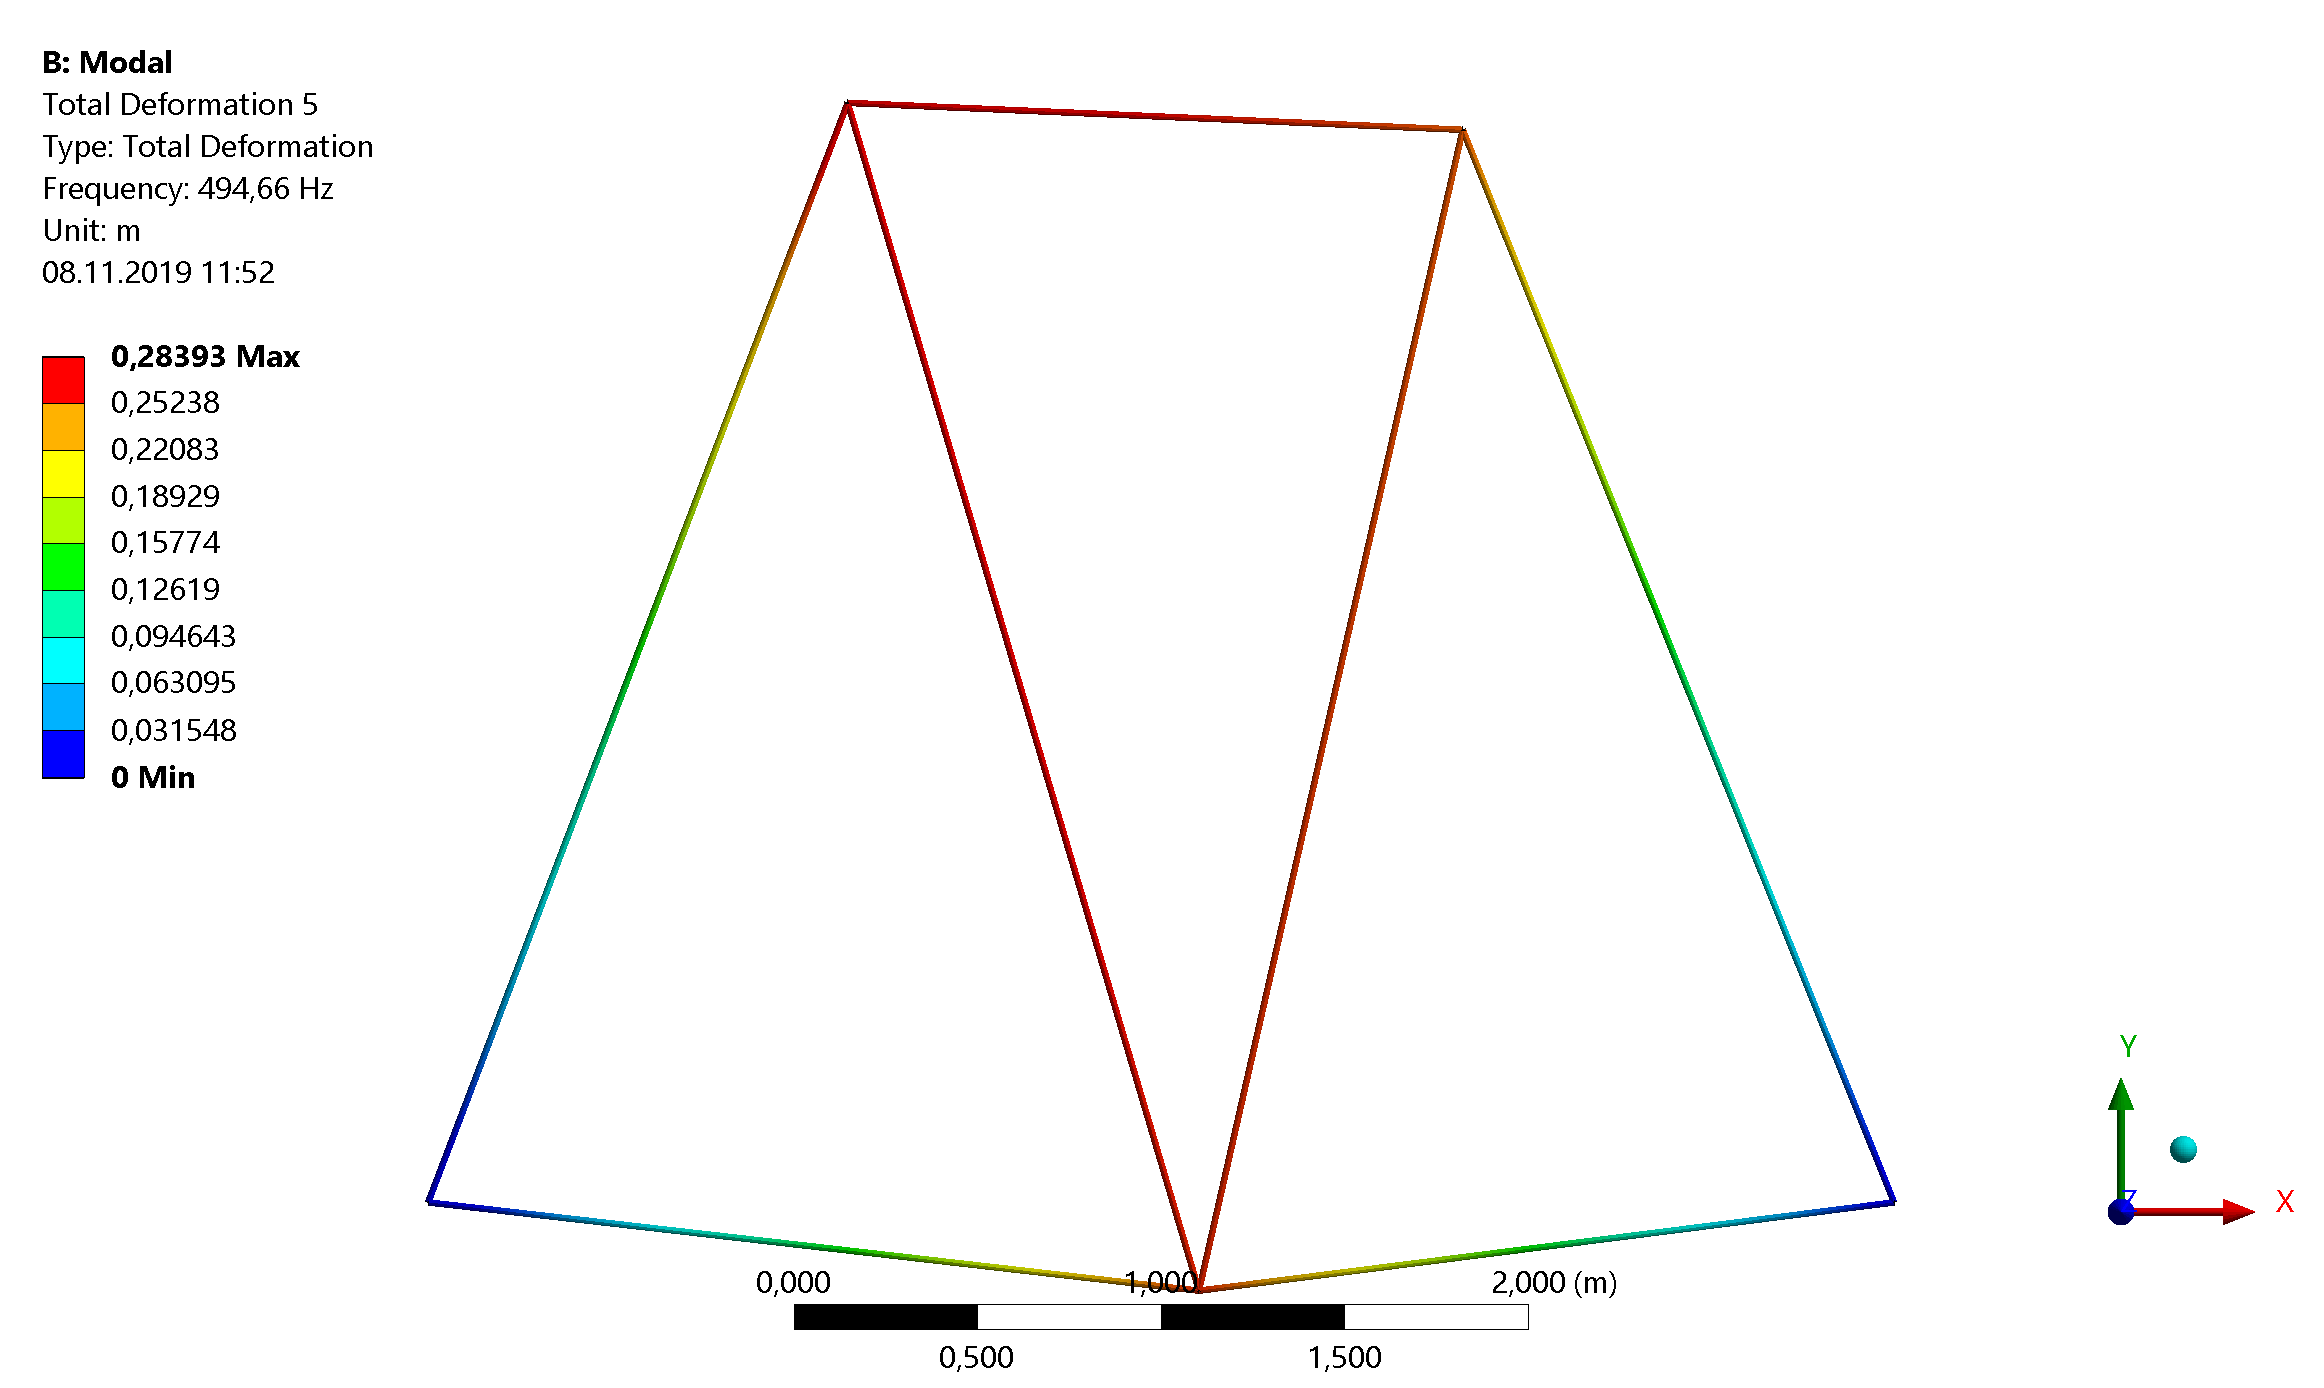
\includegraphics[width=\textwidth, height=0.6\textwidth]{mode5.png}
    \caption{Postać drgań dla $f=494,66 [Hz]$}
    \label{rys:mode5}
\end{figure}

\begin{figure}[H]
    \centering
    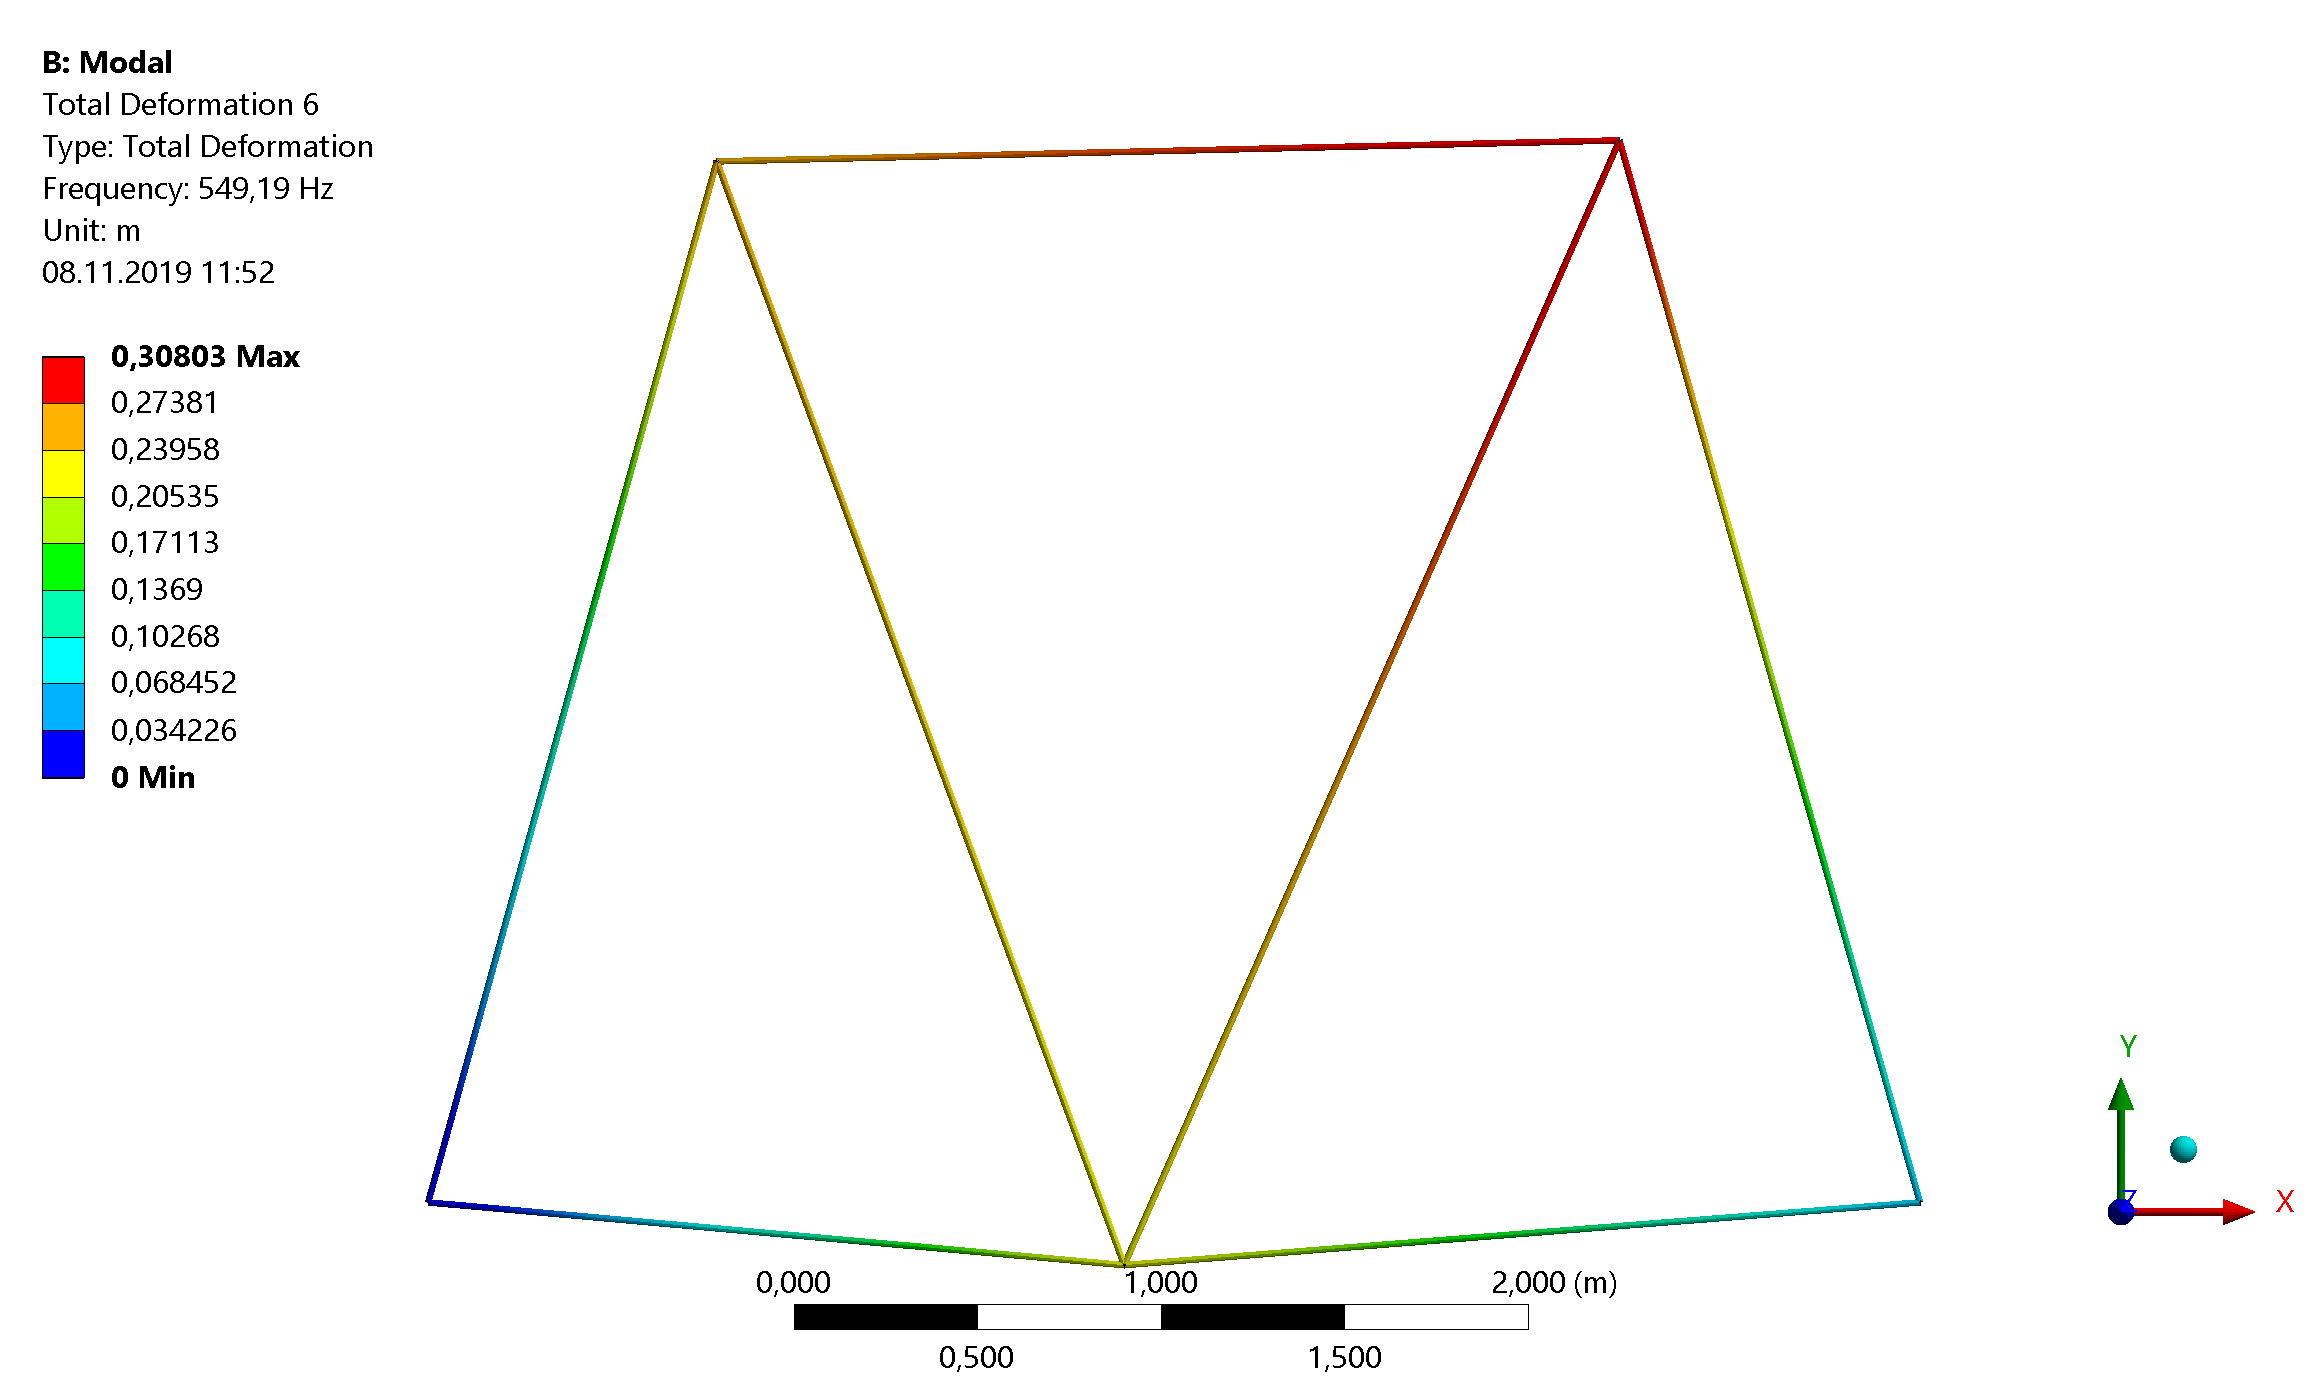
\includegraphics[width=\textwidth, height=0.6\textwidth]{mode6.png}
    \caption{Postać drgań dla $f=549,19 [Hz]$}
    \label{rys:mode6}
\end{figure}

\begin{figure}[H]
    \centering
    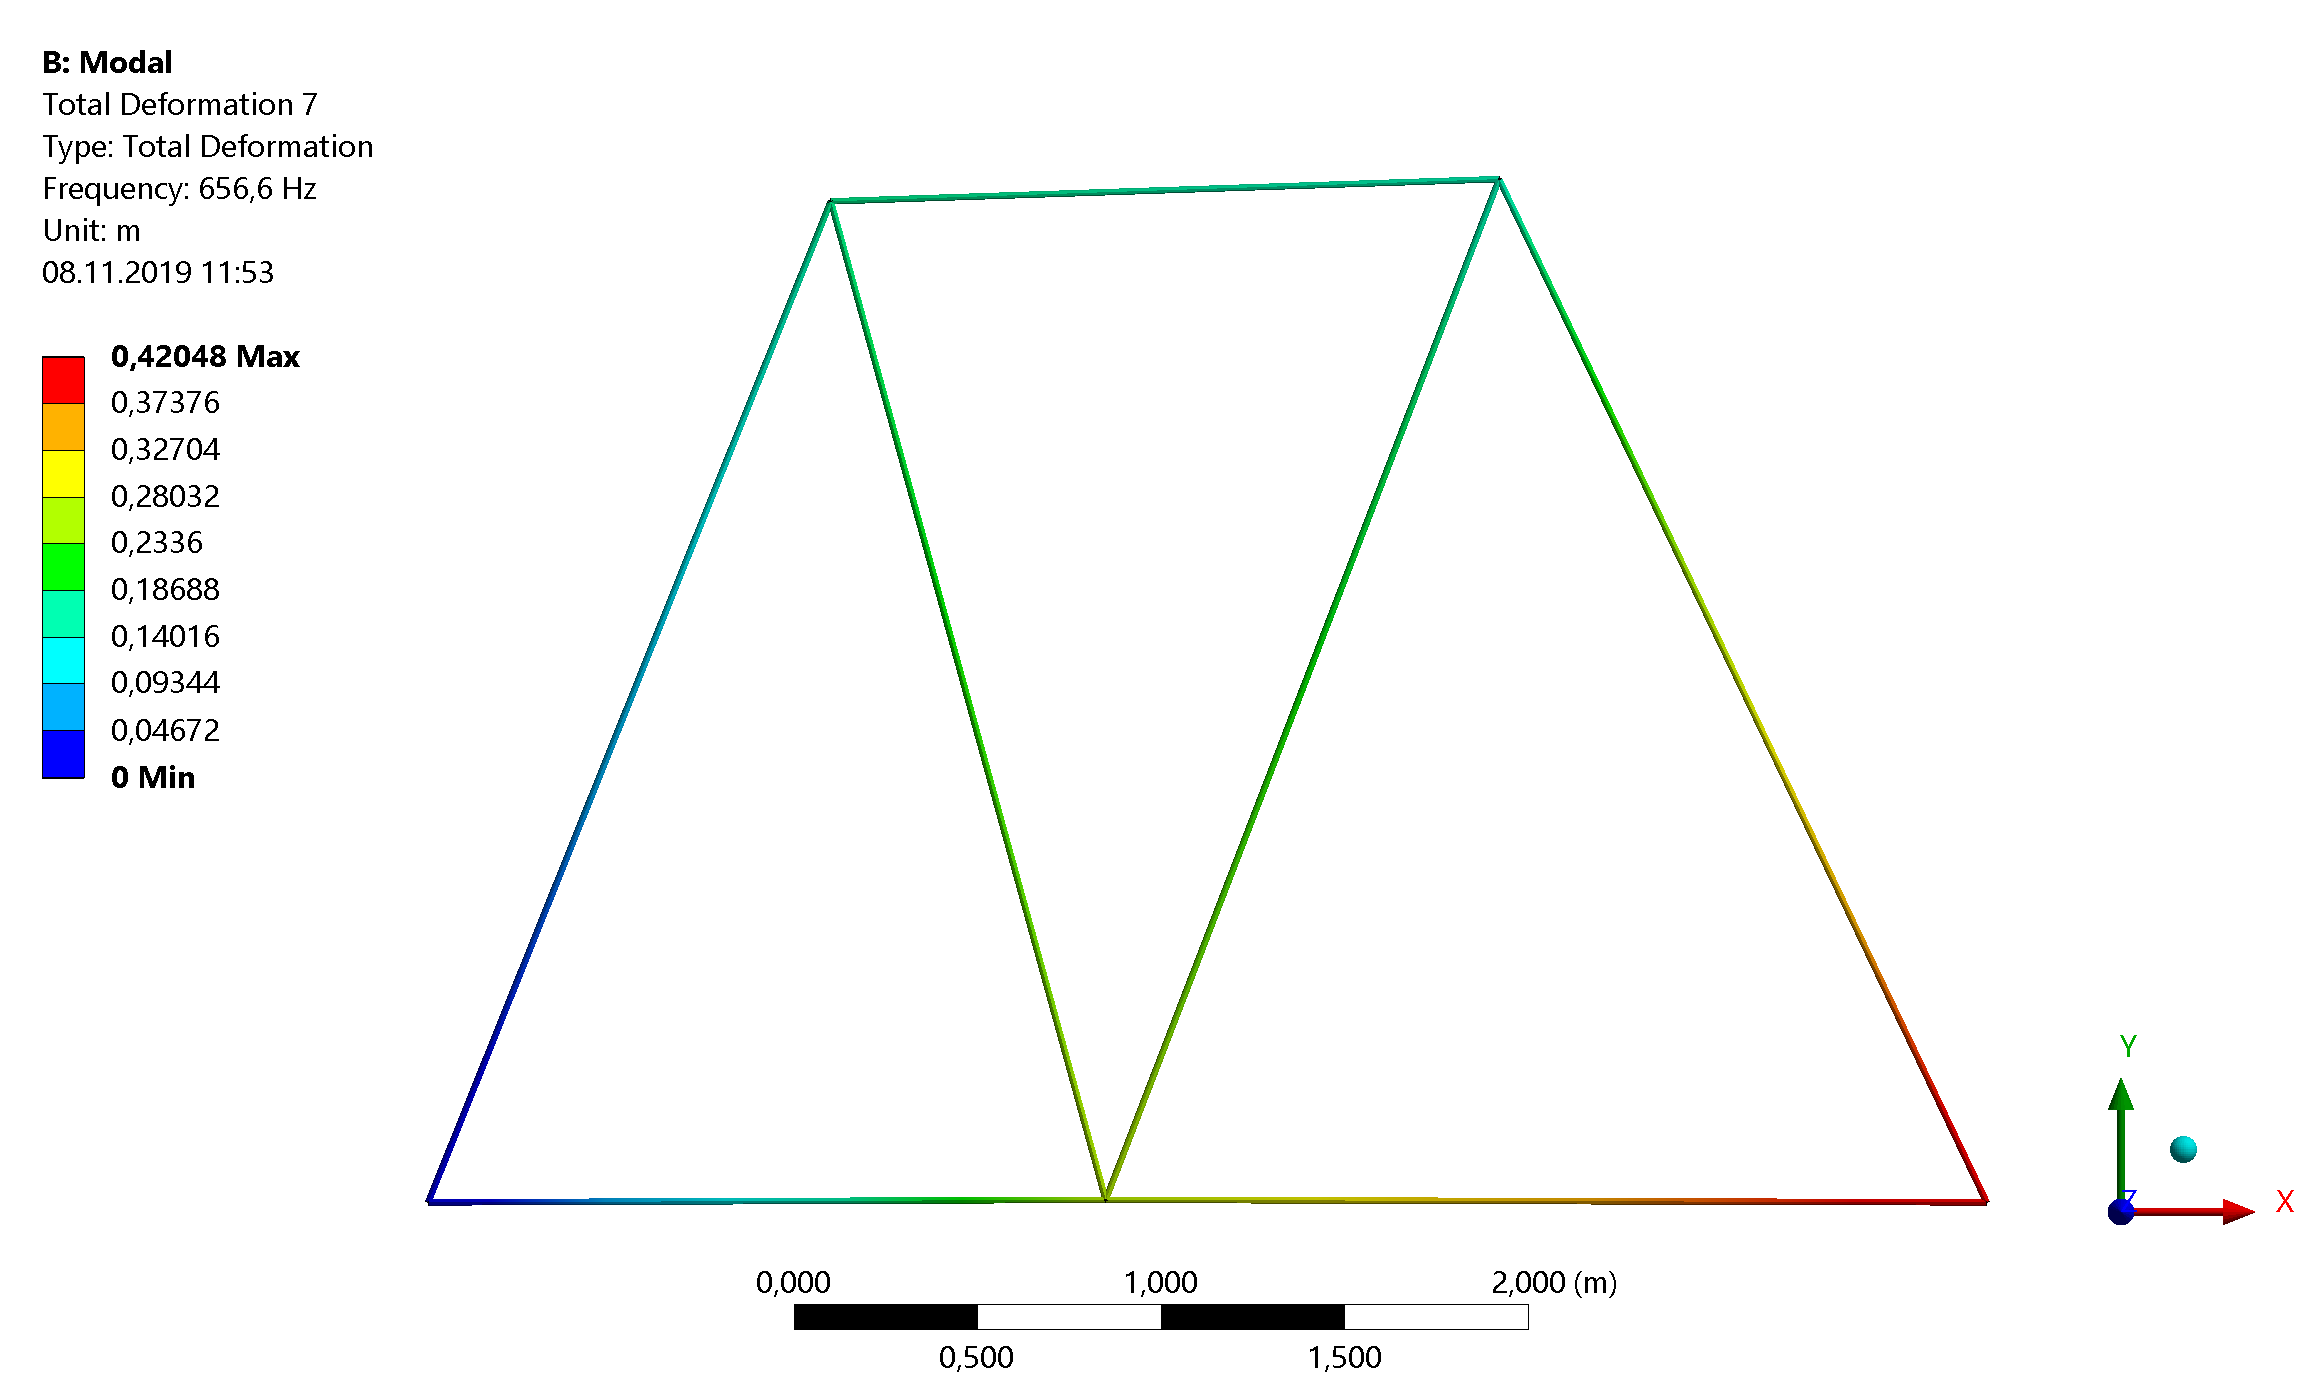
\includegraphics[width=\textwidth, height=0.6\textwidth]{mode7.png}
    \caption{Postać drgań dla $f=656,60 [Hz]$}
    \label{rys:mode7}
\end{figure}

\section{Porównanie wyników oraz wnioski}
\label{sec:wnioski}

Jak można zauważyć analiza statyczna w przypadku obu środowisk daje podobne rezulataty. Analizując rysunki \ref{rys:totaldef} oraz \ref{kratownicawynik} można zauwazyć, że odkształcenia są bardzo zbliżone oraz kształt przyjmowany przez kratownice jest spójny. W poniższej tabeli znajduje się zestawienie odpowiednich przemieszczeń dla obu modeli.

\begin{table}[H]
\centering
\label{tab:zeststat}
\caption{Zestawnie przemieszczeń węzła nr 3 z obu modeli statycznych}
\begin{tabular}{|c|c|c|}
\hline
                                                                                     & Matlab & ANSYS  \\ \hline
\begin{tabular}[c]{@{}c@{}}Przemieszczenie bezwzględne węzła\\ {[}mm{]}\end{tabular} & 78,5   & 78,55 \\ \hline
\begin{tabular}[c]{@{}c@{}}Przemieszczenie na kierunku X\\ {[}mm{]}\end{tabular}     & 7,7    & 6,81   \\ \hline
\begin{tabular}[c]{@{}c@{}}Przemieszczenie na kierunku Y\\ {[}mm{]}\end{tabular}     & -78,1  & -78,17 \\ \hline
\end{tabular}
\end{table}

Jak widać w tabeli \ref{tab:zeststat} otrzymane przemieszczenia w obu środowiskach są bardzo zbliżone i może to być podstawą do akceptacji wyników otrzymanych w środowisku Matlab. Należy zwrócić uwagę, że w przypadku bardziej skomplikowanych problemów przeprowadzenie obliczeń w taki sposób wymagało by o wiele większego nakładu pracy niż w przy uzyciu narzędzi inżynierkich jak na przykład oprogramowanie ANSYS.


Porównując wyniki analizy modalnej możemy zawuważyć ze pokrywają się częstotliwości drgań oraz kształt w obu metodach. Swiadczy to o tym, że macierze mas oraz sztywności dla wybranego typu elmentu są budowane w ten sam sposób oraz metoda wyznaczania częstotliwości własnych musi być taka sama.
Dodatkowo można zauważyć, że otrzymane wektory własne w przypadku analizy w środowisku Matlab są przemieszczeniami węzłów. Analizując przemieszenia węzłów na rysunkach ze środowiska ANSYS widoczne jest, że wartości przemieszczeń są zbliżone do tych otrzymanych pierwszą metodą co może swiadczyć o podobnej metodzie wyznaczania wektorów własnych oraz sposobie normalizacji wektorów własnych. Jest to normalizacja M-ortogonalna, ponieważ po przeprowadzeńu normalizacji względem macierzy bezwładności wektory normlane uzyskane z funkcji $eig$ nie zmieniły wartości.


\end{document}
